\documentclass[12pt,a4paper]{report}

% Packages
\usepackage[margin=1in,left=1.5in]{geometry}
\usepackage{times}
\usepackage{setspace}
\usepackage{titlesec}
\usepackage[nottoc,notlot,notlof]{tocbibind}
\usepackage{tocloft}
\usepackage{fancyhdr}
\usepackage{graphicx}
\usepackage{booktabs}
\usepackage{usecase}
\usepackage{xcolor}
\usepackage{hyperref}
\usepackage{enumitem}
\usepackage{longtable}
\usepackage{ragged2e}

\definecolor{lightgrey}{RGB}{120,120,120}

\pagestyle{fancy}
\fancyhf{}
\fancyhead[R]{\color{lightgrey}\leftmark}
\fancyfoot[C]{\thepage}

\renewcommand{\chaptermark}[1]{\markboth{Chapter \thechapter: #1}{}}
\renewcommand{\headrulewidth}{0.4pt}
\renewcommand{\headrule}{\hbox to\headwidth{\color{lightgrey}\leaders\hrule height \headrulewidth\hfill}}

\setlength{\headheight}{14.5pt}


\doublespacing

\setlist[itemize]{leftmargin=1cm}
\setlist[enumerate]{leftmargin=1cm}

\setlength{\parskip}{1em}
\setlength{\parindent}{1em}

% hide links so no color appear, but they still work
\hypersetup{hidelinks}

% Page numbering
\pagenumbering{roman}

% Title formatting
\titleformat{\chapter}{\normalfont\huge\bfseries\uppercase}{\thechapter}{20pt}{\huge}

% Document begin
\begin{document}

% Title Page
\begin{singlespace}
\begin{titlepage}
    \begin{center}
        \vspace*{1cm}
        
\includegraphics[height=1cm]{images/yu-logo.png}\\[1cm]
        {\Large\bfseries AL YAMAMAH UNIVERSITY}\\[0.5cm]
        {\large College of Engineering and Architecture}\\[0.5cm]
        {\large Bachelor of Science in Software and Network Engineering}\\[2cm]
        {\Huge\bfseries 
            \begin{spacing}{1}
                Jadwal: An Elegant, iOS-based Calendar Manager
            \end{spacing}
        }
        \vspace{2cm}
        {\Large\bfseries Graduation Project}\\[2cm]
        \begin{center}
            \setlength{\fboxsep}{10pt}
            \setlength{\fboxrule}{1pt}
            \fbox{
                \begin{tabular}{p{0.45\linewidth}p{0.45\linewidth}}
                    \multicolumn{2}{c}{\textbf{Group Project Submission}} \\
                    \midrule
                    \textbf{Student Names} & \textbf{Student IDs} \\
                    \midrule
                    YAZED ALKHALAF & 202211123 \\
                    SAIMAN TAKLAS & 202021400 \\
                    AFFAN MOHAMMAD & 202211086 \\
                    ALI BA WAZIR & 202211018 \\
                    \midrule
                    \multicolumn{2}{l}{\textbf{Submission Date}: 30 Oct 2024} \\
                    \multicolumn{2}{l}{\textbf{Supervised By}: Dr. Inayatullah} \\
                \end{tabular}
            }
        \end{center}
        \vfill
        {\large First Semester 2024--2025}
    \end{center}
\end{titlepage}
\end{singlespace}

\begin{singlespace}

\chapter*{Abstract}
\addcontentsline{toc}{chapter}{Abstract}
    
\begin{justify}
In response to the rapid globalization of modernization, time management has been a real challenge. This paper introduces Jadwal, that proposes an automatic schedule managing system where an individual can integrate multiple calendars and extract the events that have been discussed informal communication channels,such as Whatsapp
  
\textbf{Key Objectives:}
\begin{itemize}
    \item To develop an intelligent calendar management system that automatically extracts events from the informal communication channels like WhatsApp and adds them to the user's main calendar.
    \item To create a user friendly interface that allows users to easily add events to the calendar.
    \item To implement a smart resolution system that notifies users of scheduling conflicts and provides easy options for resolution.
    \item To integrate all the calendars into Jadwal's single calendar view to make viewing and managing all the events easy.
    \item To prioritize and automatically schedule daily routines such as waking time, sleeping time and prayer time.
    \item To significantly reduce the time users spend on manual calendar management.
    
\end{itemize}


\begin{center}
    The system will be a mobile application, designed for iOS devices.
    \end{center}




\end{justify}

    
\chapter*{Acknowledgment}
\addcontentsline{toc}{chapter}{Acknowledgment}
    
\begin{justify}
First and foremost, we would like to thank our Graduation project supervisor Dr. Inayathullah for his invaluable guidance and precious time. His advise was instrumental in shaping our project and by providing support in challenging times.Moreove,he emphasized that all member should involve in each phase of the project and gain core knowledge and contribute efficiently .
His stimulus and help to complete the project successful.
  


Secondly, we would like to thank all the professors and friends for their insightful recommendations which helped us to enhance our project.
    


Lastly, we would like to thank our parents for their unwavering support and for preparing us mentally and physically throughout this journey.
\end{justify}
    
\newpage

\tableofcontents

\newpage
\listoffigures


\newpage
\listoftables

\chapter*{List of Abbreviations and Terminology}
\addcontentsline{toc}{chapter}{List of Abbreviations and Terminology}

\begin{center}
    \begin{longtable}{p{0.2\textwidth}p{0.7\textwidth}}
    \toprule
    \textbf{Term} & \textbf{Definition} \\
    \midrule
    \endhead
    
    \textbf{Calendar} & A list of events and dates within a year that are important to an organization or to the people involved in a particular activity. \cite{def:calendar} \\[1ex]
    
    \textbf{Jadwal} & Jadwal is a comprehensive time management tool designed to aggregate and optimize your existing calendars and data sources. \\[1ex]
    
    \textbf{WhatsApp} & WhatsApp is an alternative to SMS and offers simple, secure, reliable messaging and calling, available on phones all over the world. \cite{whatsapp-about} \\[1ex]
    
    \textbf{CalDAV} & Calendaring Extensions to WebDAV \\[1ex]
    
    \textbf{Golang} & Go is an open source project developed by a team at Google and many contributors from the open source community. \cite{def:Golang}\\[1ex]
    
    \textbf{JWT} & JSON Web Tokens are an open, industry standard RFC 7519 method for representing claims securely between two parties. \cite{def:JWT}\\[1ex]
    
    \textbf{WebDAV} & Web Distributed Authoring and Versioning \\[1ex]
    
    \textbf{HTTPS} & HyperText Transfer Protocol Secure \\[1ex]
    
    \textbf{iOS} & iPhone Operating System \\[1ex]
    
    \textbf{N/A} & Not Applicable \\[1ex]
    
    \textbf{UC} & Use Case \\[1ex]
    
    \textbf{ER diagram} & Entity Relationship ER Diagram is a type of flowchart that illustrates how entities \\[1ex]
    
    \textbf{Sequence Diagram} & An interaction diagram that details how operations are carried out. \\[1ex]
    
    \textbf{APIs} & Application programming interface. \\[1ex]
    
    \textbf{APNs} & Apple Push Notification service \\

    \textbf{Magic Link} & A link sent via email that allows for passwordless sign in. \\
    
    \bottomrule
    \end{longtable}
\end{center}

\end{singlespace}

% Main body (switch to Arabic numerals)
\pagenumbering{arabic}

\chapter{Introduction}


\section{Background of the Project}

 Calendars have been around a long time now, and they are a handy tool for humans. Both who are busy and who want to plan their days. People throughout history have used paper for calendars, but now with technology, things have changed. Calendars are digital now, and they can even be shared with others!

As the world is becoming one big village with globalization, people tend to squeeze every last minute of their days since competition is higher. Calendars help in that since they allow people to plan their days easily and keep track of when to meet people and do other activies.

People these days use multiple calendars and sometimes forget to insert an event to the correct calendar.
\section{Problem Statement}

Keeping your calendar up to date with event information is challenging, especially with the rise of many informal communcation channels like WhatsApp. People nowadays discuss when and where they will meet using those informal communication tools. This leads to calendars being out of sync from real life events you are committed to and might harm relations. The problem lies in the cumberness of adding events to a calendar manually, and sometimes people are busy, you just forget that you didn't add the event to your calendar. Our Jadwal app aims to solve this issue for users in an elegant way that makes it seamless to manage your time confidently.

\section{Objectives of the Project}

The main objectives of Jadwal are:
\begin{itemize}
    
    \item To integrate all the calendars into Jadwal's single calendar view to make viewing and managing all the events easy.
    \item To develop an intelligent calendar management system that automatically extracts events from the informal communication channels like WhatsApp and adds them to the user's main calendar.
    \item To significantly reduce the time users spend on manual calendar management.
    \item To create a user friendly interface that allows users to easily add events to the calendar.
    \item  To prioritize and automatically schedule daily routines such as waking time, sleeping time and prayer time.
    \item To implement a smart resolution system that notifies users of scheduling conflicts and provides easy options for resolution.
\end{itemize}

\section{Scope of the Project}

Jadwal is not just another calendar application; it's a comprehensive time management tool designed to aggregate and optimize your existing calendars and data sources. The scope of the project includes:
\begin{itemize}
    \item Development of an iOS application as the primary platform.
    \item Integration with calendars using CalDAV.
    \item WhatsApp message parsing for event extraction (subject to technical feasibility).
    \item Target audience: Busy professionals, students, and anyone juggling multiple schedules.
    \item User testing phase to ensure ease of use and effectiveness. Our testing methods will include:
    \begin{itemize}
            \item Beta testing with a diverse group of users.
            \item Analytics to track user behavior and app performance.
        \end{itemize}
\end{itemize}


\section{Significance of the Project}

Jadwal's significance can be summarized in the following points:
\begin{enumerate}
    \item \textbf{Time is Money}: Since time is the only asset you can't get more of, Jadwal tries to make it less painful and less time consuming to have a good calendar throughout your day by parsing events from your informal communication channels like WhatsApp automatically.
    \item \textbf{Prayer First Calendar}: Prayer times come first, then your daily scheduled items.
    \item \textbf{Reduced Human Error}: Automated event extraction and addition to calendars minimize the risk of missing important events or appointments due to manual input errors or forgetfulness.
    \item \textbf{Conflict Resolution}: The smart resolution system helps users identify and resolve scheduling conflicts efficiently, reducing stress and improving overall time management.
    \item \textbf{Holistic View of Commitments}: By integrating multiple calendars into a single view, Jadwal provides users with a comprehensive overview of their commitments across various aspects of life, facilitating better decision-making and work-life balance.
\end{enumerate}

\section{Limitations of the Project}

Nothing is perfect, and our project is not an outlier. The limitations we have figured out about it are as follows:
\begin{itemize}
    \item WhatsApp integration allows the app to read the users messages, so it would be difficult to prove that privacy risk associated with our integration isn't compromised.
    \item WhatsApp integration might not always be there, they are a third-party.
    \item Learning new technologies for iOS development might require more time than anticipated.
    \item Accuracy of our algorithms to detect keywords indicating an event agreement has happened, especially for languages other than English.
    \item Time and manpower constraints may limit the number of features we can implement.
    \item Dependency on third-party APIs and their limitations.
    \item We may face a challenges to test the app due to lack of users for testing our app
\end{itemize}

\newpage

\section{Organization of the Senior Project}

Our project plan can be illustrated in the following gantt chart, \textbf{Figure \ref{fig:project-gantt-chart}}.

\begin{figure}[!h]
    \centering
    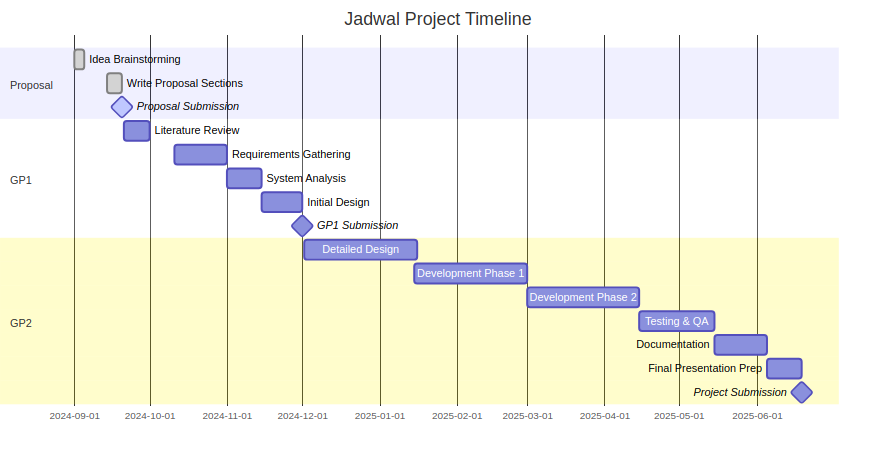
\includegraphics[width=\textwidth]{images/gantt.png}
    \caption{Project Gantt Chart}
    \label{fig:project-gantt-chart}
\end{figure}

\section{Conclusion}

In conclusion, the shift from traditional calendars to digital ones has changed how people organize their schedule. While digital calendars offer easy and conflict free scheduling which makes managing easy. Discussion on informal communication channels like WhatsApp has impacted the planning events and commitments. This impact often leads to missed appointments and scheduling conflicts, especially for someone who is busy.

Jadwal aims to solve this issue by providing a seamless and automated solution for integrating informal communication with the application so that no one misses an event and have conflicts. 

\chapter{Literature Review}

\section{Introduction}
In the modern world, managing time effectively is important for balancing personal and professional responsibilities. The increasing complexity of schedules usually results in missing an important event and overlapping commitments. To solve these challenges, we introduce Jadwal, an innovative iOS-based schedule management application, aims to help individuals and professionals to organize their daily lives.
Jadwal focuses on solving the issue by drawing inspiration from existing solutions like Clockwise, Motion, Reclaim AI, and Calendi, Jadwal outstands by introducing advance features such as conflict resolution, task prioritization, event extraction from informal communicating channels and prioritizing prayer times, which is a unique feature which is not found in any competing applications. 

In developing Jadwal, we have drawn inspiration from and built upon existing research and products in the field of intelligent calendar management. Some key references include:
\begin{itemize}
    \item \textbf{Clockwise (https://www.getclockwise.com/):} A smart calendar assistant that optimizes schedules and manages team coordination \cite{clockwise}. Clockwise's approach to intelligent time blocking and meeting optimization provides valuable insights for Jadwal's automated scheduling features.
    \item \textbf{Motion (https://www.usemotion.com/):} Motion's Intelligent Calendar takes your meetings, your tasks, your to-do list, your activities, and creates one perfect, optimized schedule to get it all done \cite{motion}.
    \item \textbf{Reclaim AI (https://reclaim.ai/):} An intelligent time management tool that helps optimize schedules and automate tasks \cite{reclaim}.
    \item \textbf{Calendi (https://calendi.ai/):} Calendi describes itself as: ``Calendi is an AI calendar system. Use it for scheduling tasks, automating meetings, and witness the future of calendar.'' \cite{calendi}
    \item \textbf{An Exploratory Study of Calendar Use:} ``Prospective remembering is the use of memory for remembering to do things in the future, as different from retrospective memory functions such as recalling past events.'' \cite{tungare2008exploratorystudycalendaruse}
    \item \textbf{WhatsApp Integration:} Our research indicates that direct WhatsApp integration for event extraction has not been widely implemented in existing calendar applications, making this a unique feature of Jadwal.
\end{itemize}

\begin{figure}[!h]
    \centering
    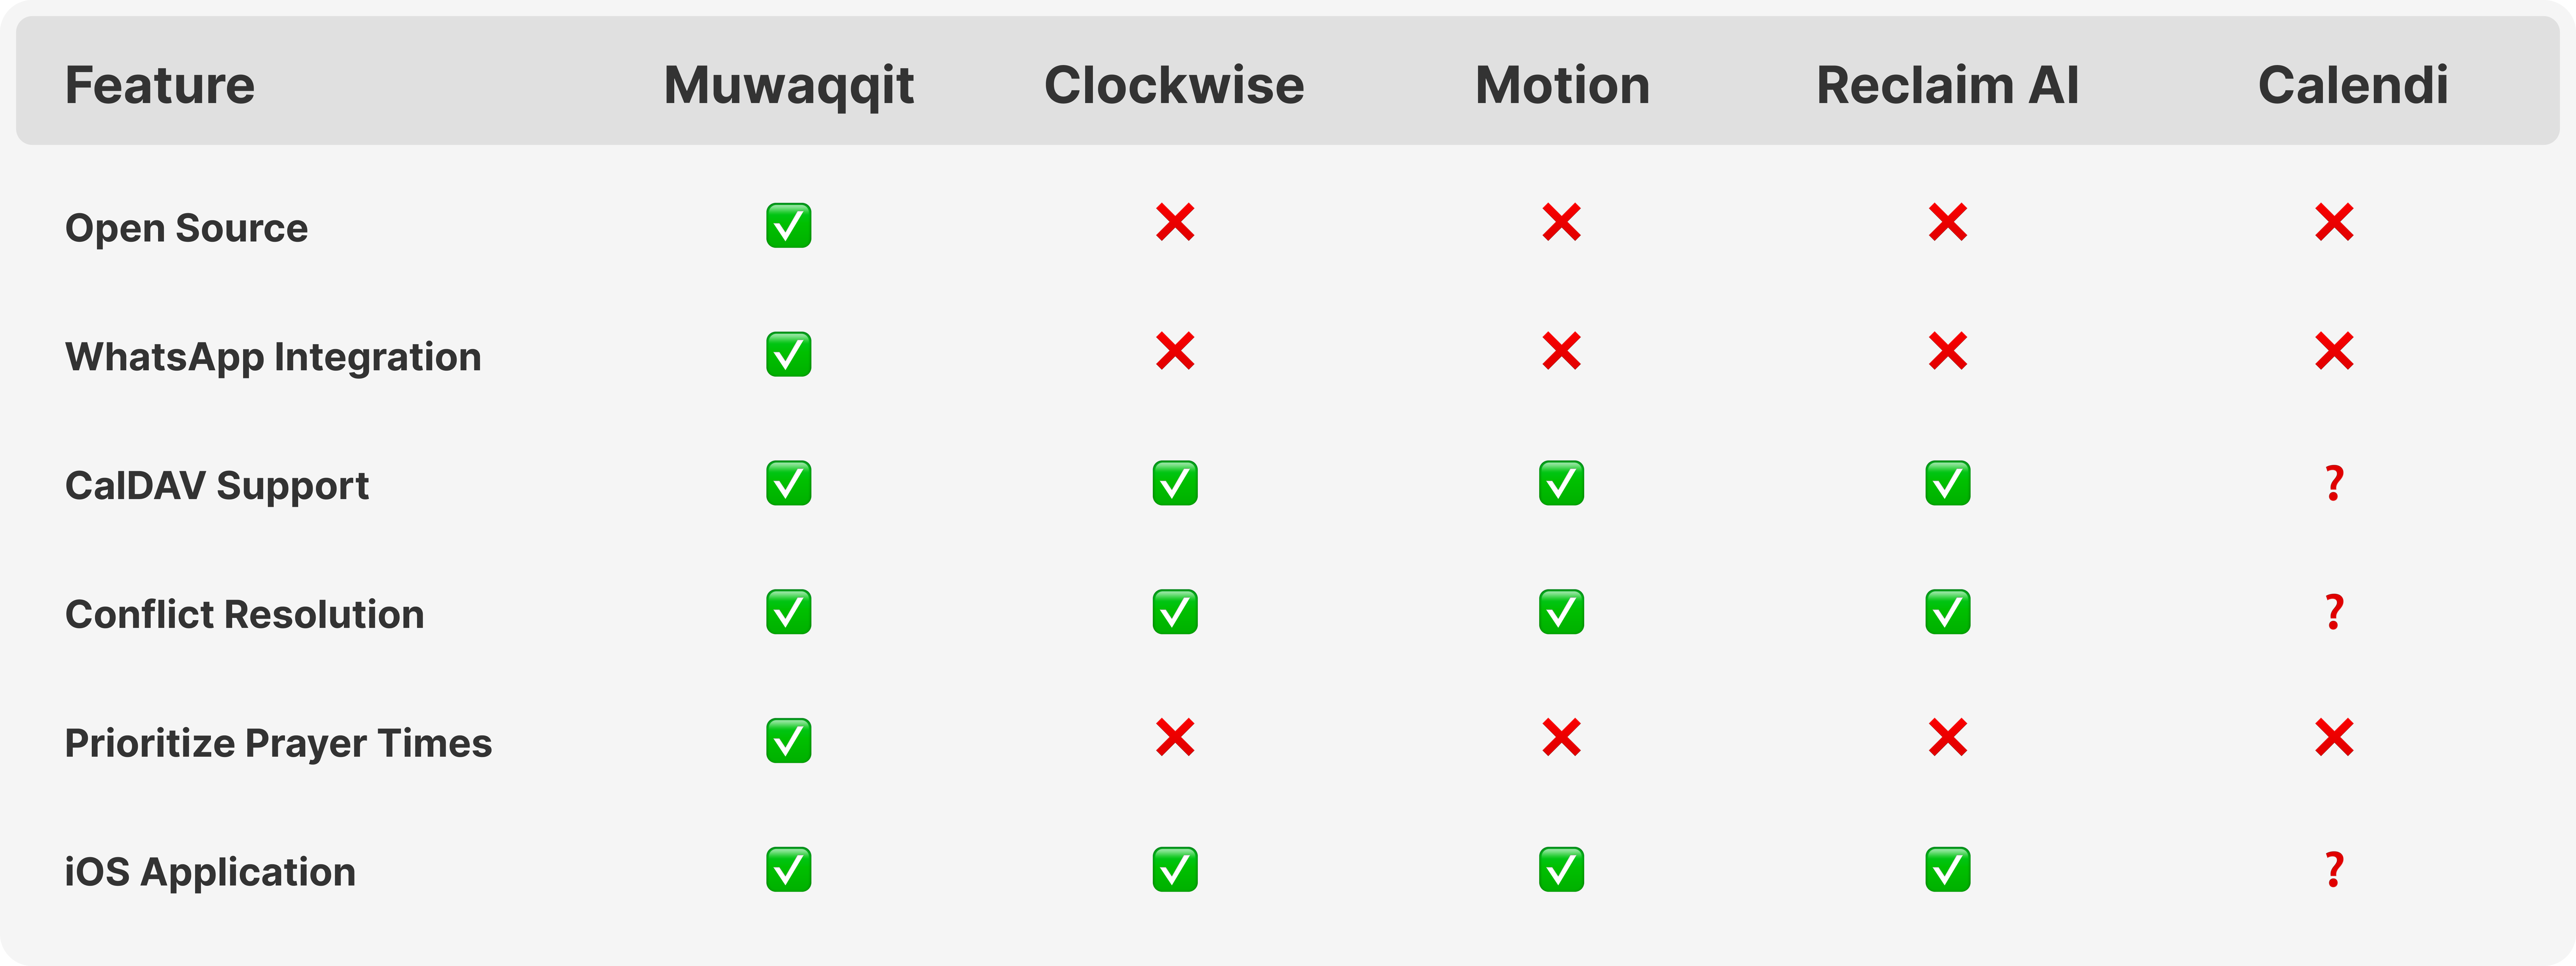
\includegraphics[width=\textwidth]{images/features-table.png}
    \caption{Feature Comparison Table}
    \label{fig:features-table}
\end{figure}

\newpage

In Figure \ref{fig:features-table} The table compares \textit{Jadwal}, our project, with four other scheduling applications—Clockwise, Motion, Reclaim AI, and Calendi—based based on several key features:
\begin{itemize}
    \item \textbf{Open Source}: \textit{Jadwal} stands out as the only application that is open-source, allowing users and developers to access, modify, and improve the code. The other applications do not provide this.
    \item \textbf{WhatsApp Integration}: \textit{Jadwal} stands out again as the only application that connects and extract the event discussed over the platform by the user.
    \item \textbf{CalDAV Support}: \textit{Jadwal}, Clockwise, and Reclaim AI offer CalDAV support, which allows users to integrate calendars from different sources, while Motion and Calendi either does not sipport this.
    \item \textbf{Conflict Resolution}: All listed applications, including \textit{Jadwal}, supports conflict resolution, allowing users to manage overlapping events efficiently.
    \item \textbf{Prioritize Prayer Times}: \textit{Jadwal} is the only one offering this feature where the user be able to have prayer time scheduled
    \item \textbf{iOS Application}: \textit{Jadwal} is available on iOS, along with Clockwise, Reclaim AI, and Motion. The availability of Calendi on iOS is uncertain.
\end{itemize}

\section{Comparing Competitors}

Below we will compare competitors in depth, before we have only talked about them in general and shown a features comparison table.

\subsection{Clockwise}

Clockwise websites shows that they have the following feature. This feature can log in to your account, register hours and submit them from any location.

Clockwise is a platform for managing employees' working hours, requesting and managing vacation time, and sending detailed schedules. All of these features allow users to organize their lives comfortably, but Clockwise lacks some of the features found in the jadwal platform, which is linking the calendar to WhatsApp to automatically add events to the calendar. This saves the user time and organizes his day better. jadwal also has the feature of adding prayer times.

\subsection{Motion}

The Motion website states that their platform offers the following features: Motion is an AI-powered productivity tool that organizes your tasks, schedules, and meetings into a single platform. Its features include a dynamic calendar that automatically prioritizes tasks, suggests optimized schedules, and helps users adapt to changes seamlessly. The tool also provides team collaboration features, allowing shared schedules and streamlined task management to enhance team productivity. These features ensure that users can achieve maximum efficiency with minimal effort, but Motion lacks some of the features found in the 

Jadwal platform, such as linking the calendar to WhatsApp for automatic event addition and integrating prayer times, which adds a unique level of customization and day organization.

\subsection{Reclaim AI}

Reclaim.ai offers the following features: It is an AI-powered platform designed to manage tasks, habits, meetings, and personal events seamlessly. Reclaim.ai provides features such as smart time blocking, which automatically schedules tasks based on their priority and deadlines, integrates with tools like Google Calendar, Slack, and project management platforms (e.g., Asana, Jira, and Todoist), and supports habit tracking with auto-rescheduling to adapt to life changes. The platform includes calendar sync capabilities to merge multiple schedules, ensuring users avoid overbooking and manage their availability effectively. Additionally, it allows flexible privacy settings, detailed analytics for productivity tracking, and people analytics for team time management

While these features enhance productivity and optimize time management, Reclaim.ai does not include features like WhatsApp integration for automatically adding events or prayer time scheduling, both of which are unique to the Jadwal platform. These features provide users with cultural and practical benefits that further enhance their daily organization.

\subsection{Calendi}

Calendi.ai offers features focused on speeding up scheduling with AI-powered assistance. It allows users to add tasks via text or voice input and automates meeting scheduling, including sending links and calendar invites. Calendi integrates with platforms like Google Calendar, Apple Calendar, and Outlook, making it compatible across multiple systems. It provides intelligent assistance by analyzing habits and tasks, suggesting improvements, and incorporating external factors like weather or transit schedules. However, it does not offer unique features like WhatsApp integration or prayer time scheduling, which are distinct to Jadwal.

\section{Survey Results}

We have conducted a survey using Google Forms, and have sent it out to our peers in the university, and also shared it on our social media, especially LinkedIn, to get more diverse responses. That is since our main audiences are students, employees, and who do both at the same time. The results were fascinating. Especially since 75 responses were recorded with their email to authenticate the responses.

As shown in Figure \ref{fig:survey-status}, the results showed that 8\% only were both employed and students, while 53\% were students only and 39\% were employed only. We beleive this is a good mix between the two audeince we are aiming to get responses from.

\begin{figure}[!h]
    \centering
    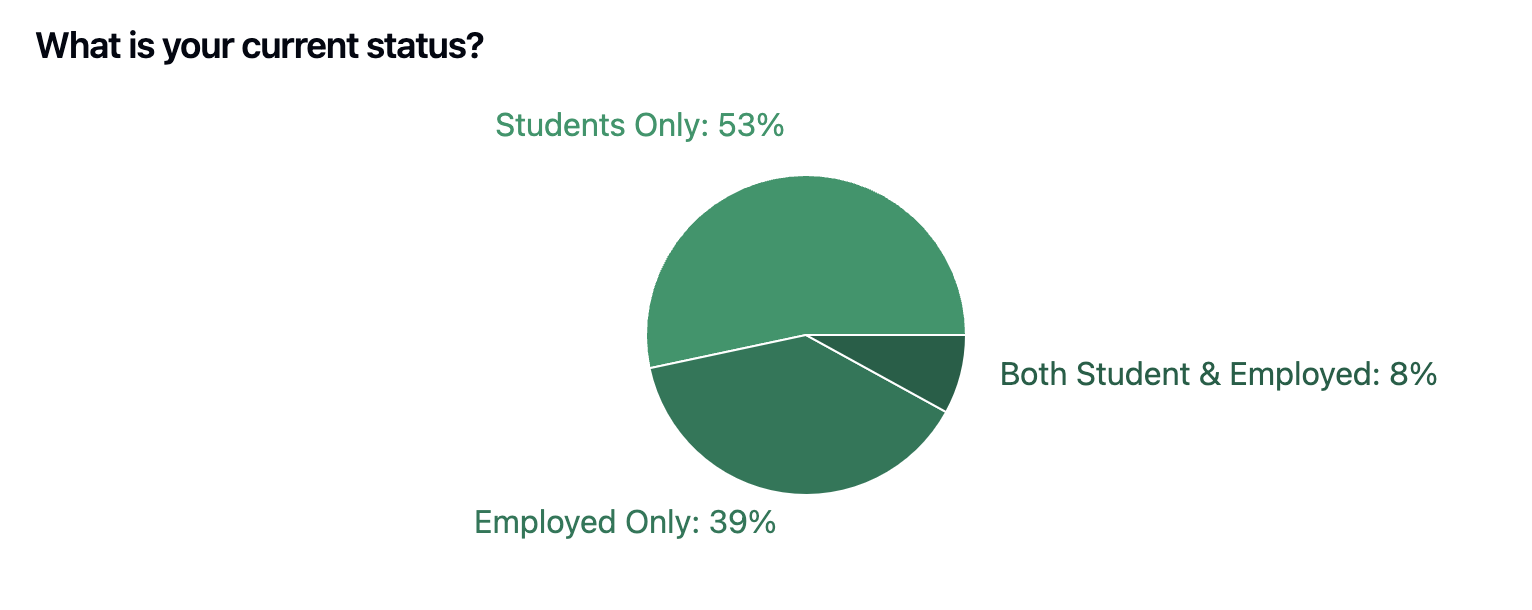
\includegraphics[width=0.8\textwidth]{images/survey/status.png}
    \caption{Survey Respondents Status}
    \label{fig:survey-status}
\end{figure}

Based on Figure \ref{fig:age-range}, it is important to note that 72\% of our respondents were of the age range 20-30 years.

\begin{figure}[!h]
    \centering
    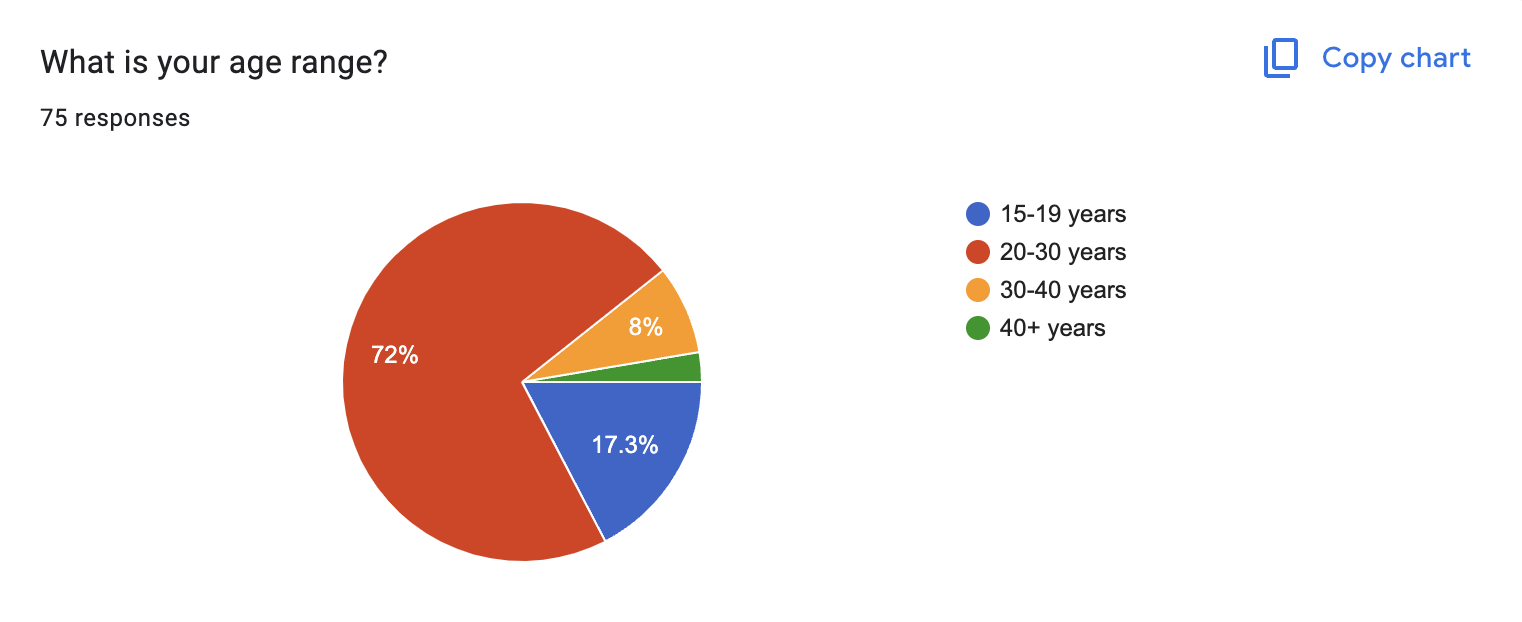
\includegraphics[width=0.8\textwidth]{images/survey/age.png}
    \caption{Age Range}
    \label{fig:age-range}
\end{figure}

As shown in Figure \ref{fig:use-calendar}, 66.7\% of people reported that they a calendar application to manage their daily schedule. This shows that people might be interested in a better way of managing their schedules that could elevate their time management skills.

\begin{figure}[!h]
    \centering
    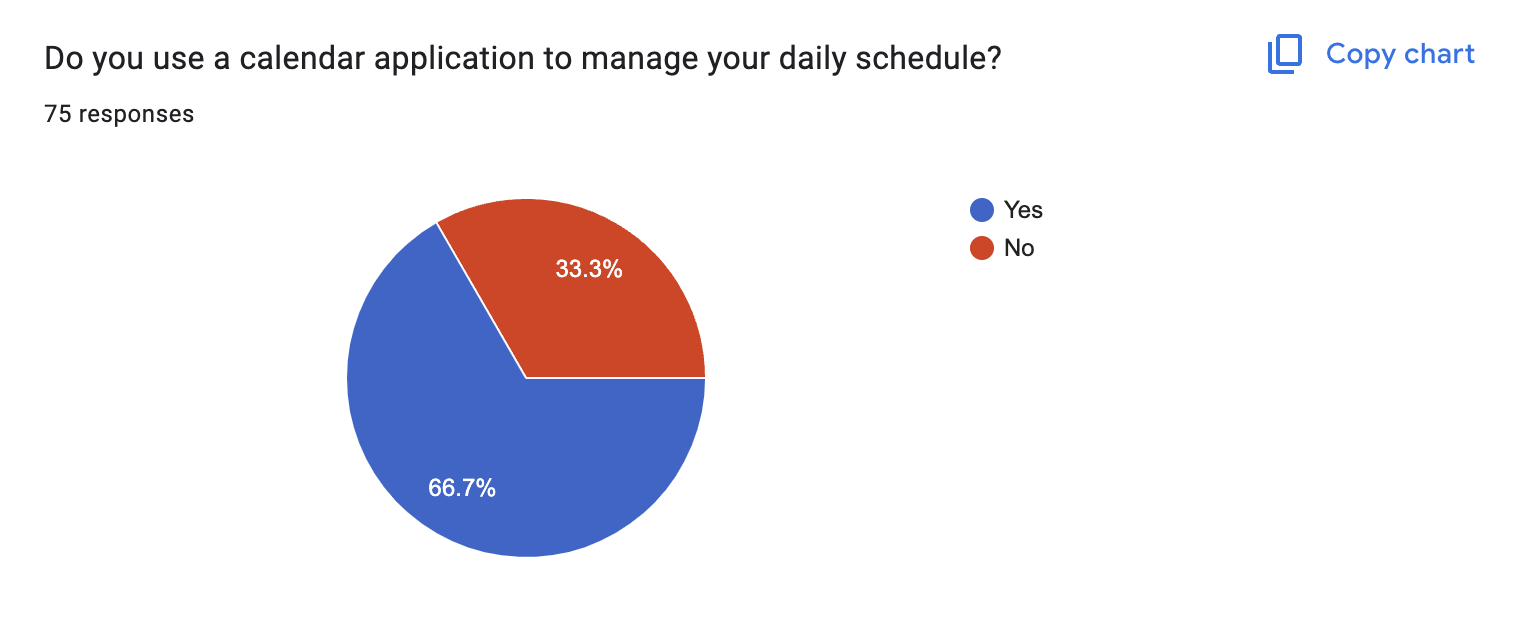
\includegraphics[width=0.8\textwidth]{images/survey/use-calendar.png}
    \caption{Percentage of People Who Use Calendars to Ones Who Don't}
    \label{fig:use-calendar}
\end{figure}

In Figure \ref{fig:platform-to-discuss}, the results showed us the need for our app to exist, since 70.7\% of the population use WhatsApp to discuss upcoming events! Another big percentage, 53.3\% used Email also. Our app won't be focusing on this, nevertheless, this is also an oppurtunity in the future to help those people who use Emails and might not find the flow easy to schedule the events in the calendar.

\begin{figure}[!h]
    \centering
    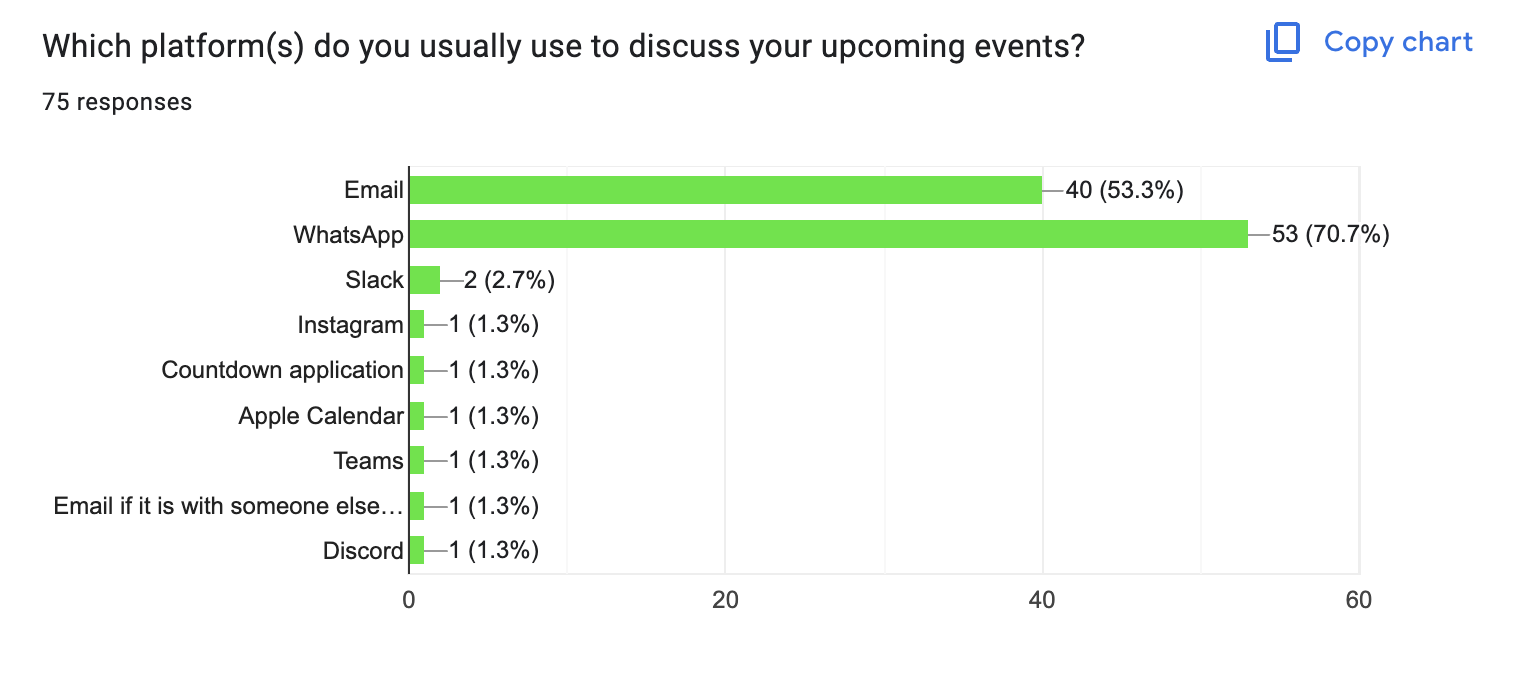
\includegraphics[width=0.8\textwidth]{images/survey/platform-to-discuss.png}
    \caption{Platform Used to Discuss}
    \label{fig:platform-to-discuss}
\end{figure}

Although 21.3\% might not seem like a lot, but as shown in Figure \ref{fig:usefullness}, 58.7\% of the population reported they would find it extremely useful to have a WhatsApp integration that automatically adds events from your conversations to the calendar?

\begin{figure}[!h]
    \centering
    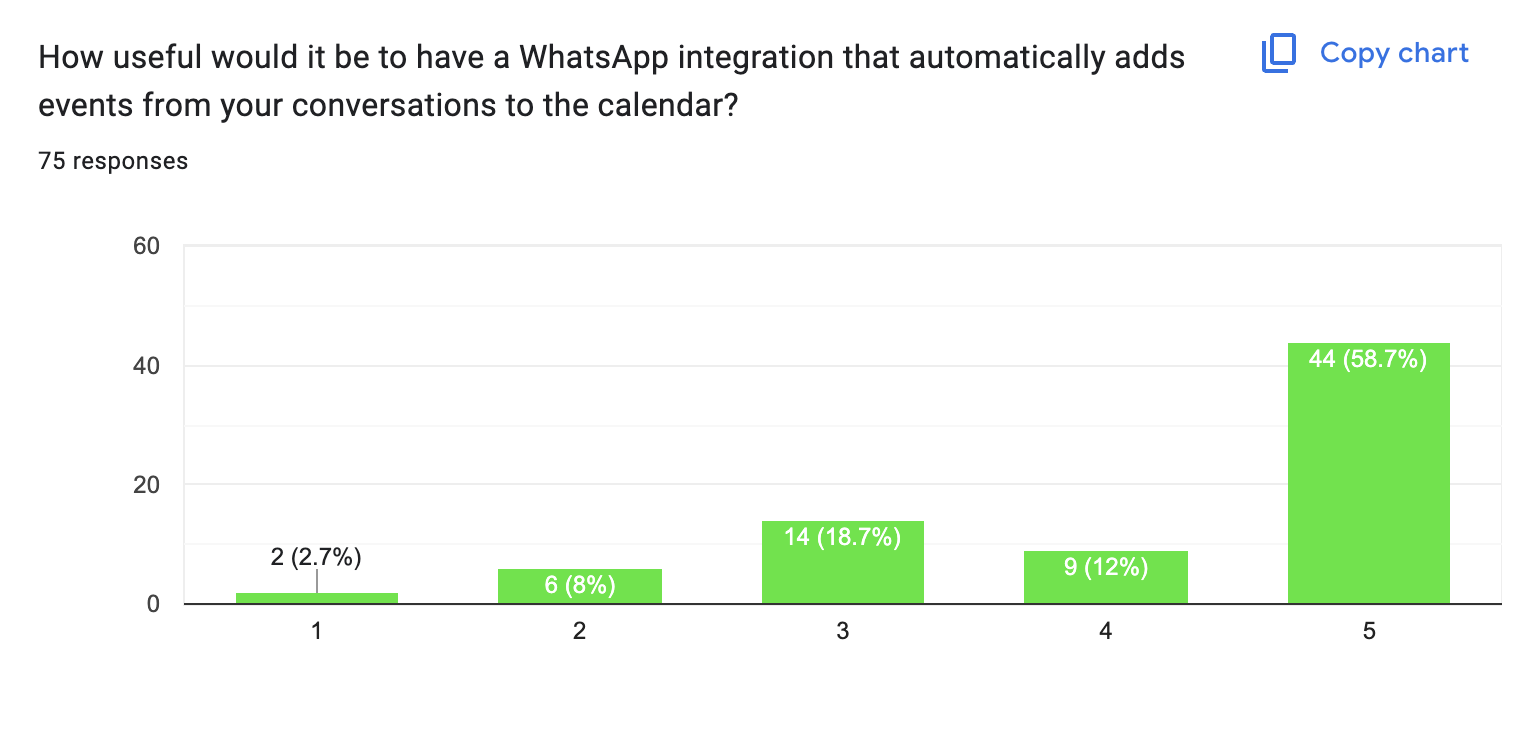
\includegraphics[width=0.8\textwidth]{images/survey/usefullness.png}
    \caption{Usefullness of Having a WhatsApp Integration}
    \label{fig:usefullness}
\end{figure}

As shown in Figure \ref{fig:forget-to-add}, on average, 21.3\% forget to add events to their calendar. That is great news, since our differentiating factor is the direct WhatsApp integration that should be able to solve this.

\begin{figure}[!h]
    \centering
    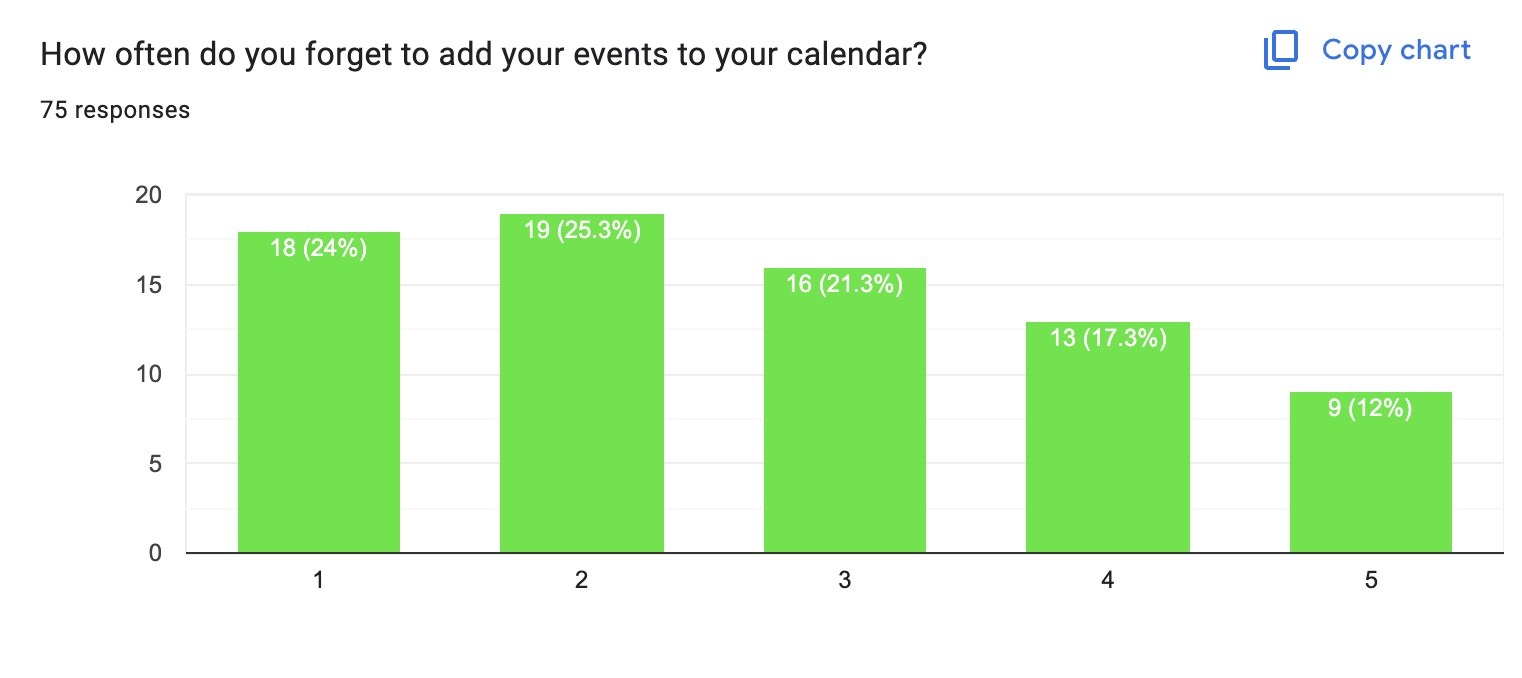
\includegraphics[width=0.8\textwidth]{images/survey/forget-to-add.png}
    \caption{Chart of Forgetting to Add Likeliness}
    \label{fig:forget-to-add}
\end{figure}

As shown in Figure \ref{fig:number-of-calendars}, 41.3\% use 2 calendars, that shows the need for a integared view of calendars.

\begin{figure}[!h]
    \centering
    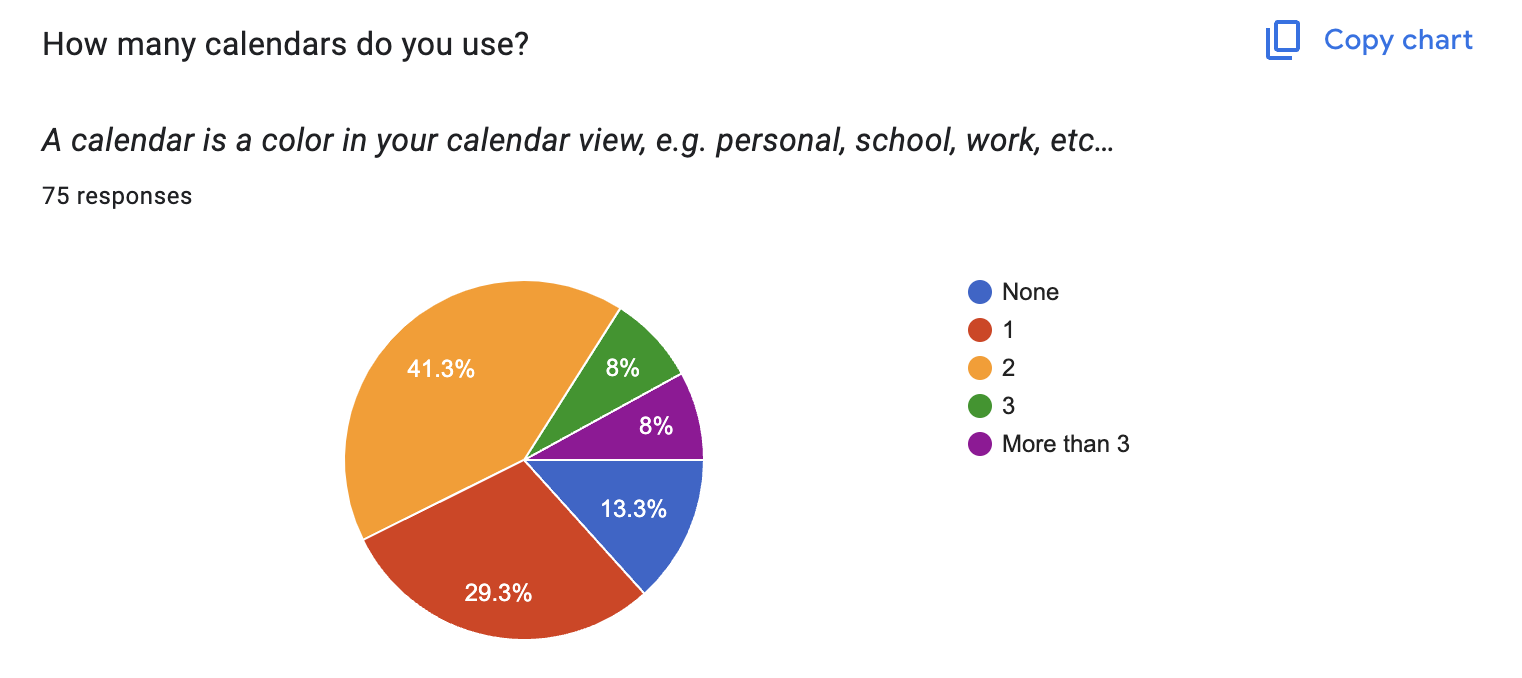
\includegraphics[width=0.8\textwidth]{images/survey/number-of-calendars.png}
    \caption{Number of Calendars}
    \label{fig:number-of-calendars}
\end{figure}

As shown in Figure \ref{fig:events-per-week}, 53.3\% of people have 1-3 calendar events per week. That might seem a little, but 33.3\% have 4-6 calendar events per week.

\begin{figure}[!h]
    \centering
    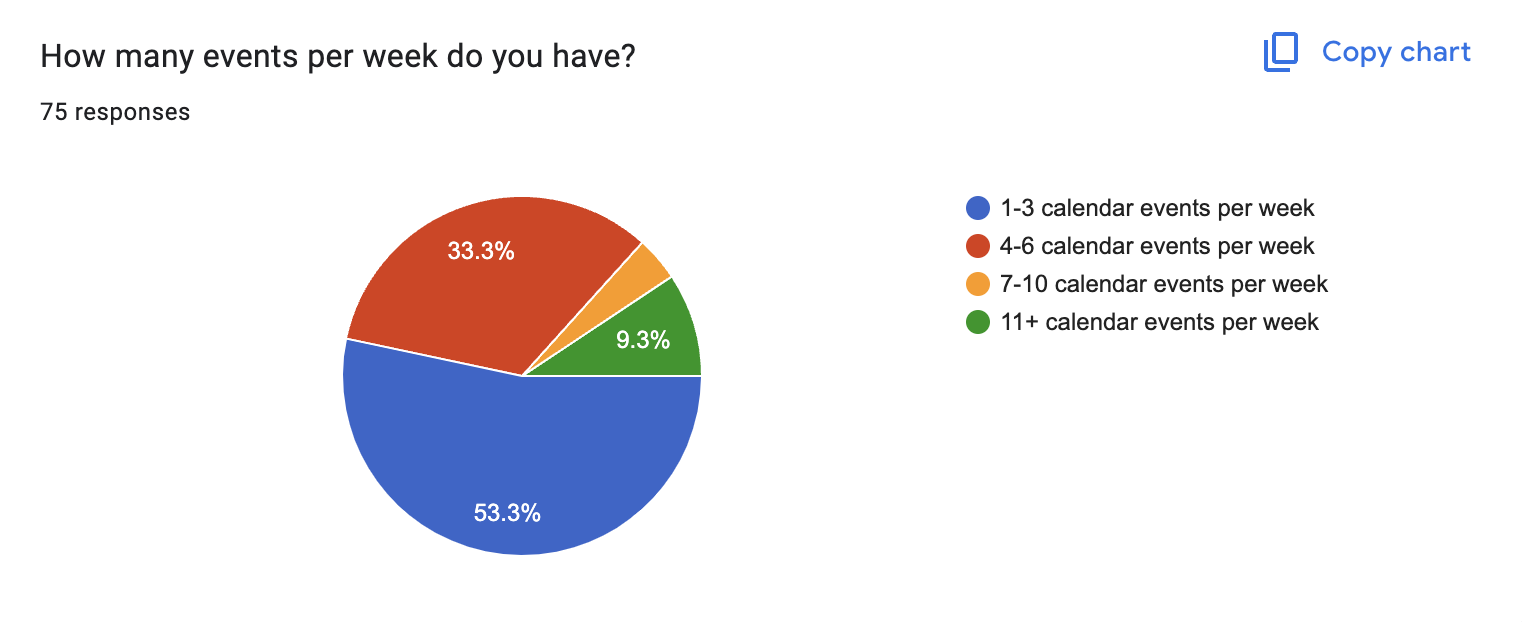
\includegraphics[width=0.8\textwidth]{images/survey/events-per-week.png}
    \caption{Events per Week}
    \label{fig:events-per-week}
\end{figure}

\section{Conclusion}

Jadwal represents itself by offering a seamless calendar application which is user friendly and outstands by providing solution to all the problems which is not yet addressed by other tools like Clockwise, Motion, Reclaim AI, and Calendi. WhatsApp integration is Jadwal’s unique features for event extraction. These features distinguish Jadwal from existing applications, Jadwal addresses to the issues that is not yet solved.

The comparison highlights Jadwal's abilities that integrate multiple calendars, resolve scheduling conflicts. 

\chapter{System Analysis and Design}

\section{Introduction}

A well-designed system requires a good understanding of both functional and non-functional requirements to meet user expectations and deliver a seamless experience. Jadwal, an iOS-based intelligent scheduling application. 

This section shows the functional and non-functional requirements which is the backbone of Jadwal's development. The functional requirements focus on core features, such as user authentication, calendar integration and event management. Ensuring the users can effectively manage their schedules. The non-functional requirements focuses on performance, security, compatibility, and user experience, ensuring the application stands well with the industry standards by providing efficient interface.

Combining all these requirements helps in the design and implementation of Jadwal which will lead to a better application solving real issues and meeting the needs of the user.


\section{Functional Requirements}

\begin{itemize}
    \item The user shall be able to access their account using either Google OAuth or magic link via Email. For new users, a new accout is created, and for existing users, they are given access to their account directly.
    \item The system shall send a welcome email to new users.
    \item The user should be able to create a calendar.
    \item The user should be able to connect a calendar using CalDAV.
    \item The user should be able to connect their WhatsApp account.
    \item The user should be able to add events manually.
    \item The user should be able to view integrated calendar.
    \item The user should be able to manage scheduling conflicts.
    \item The user should be able to schedule prayer times.
    \item The system shall send event notifications to the user.
    \item The system shall add the WhatsApp extracted events to the calendar. If a conflict occurs, the user shall get a notification to resolve the conflict with suggestions.
\end{itemize}

\newpage

\section{Non-Functional Requirements}

\begin{itemize}
    \item \textbf{Platform Compatibility:} The app shall be compatible with iOS devices running iOS 16.0 or later.
    \item \textbf{Performance:} The app shall load the main calendar view within 3 seconds on 5G with speeds above 200mpbs.
    \item \textbf{User Experience:} The user interface shall follow iOS Human Interface Guidelines for consistency and ease of use.
    \item \textbf{Security:} All data transmissions between the app and servers shall be encrypted using HTTPS.
\end{itemize}
\newpage
\section{System use-cases}
   
\textbf{Figure \ref{fig:use-case-diagram}} shows the use case diagram for the system of Jadwal.

\begin{figure}[!h]
    \centering
    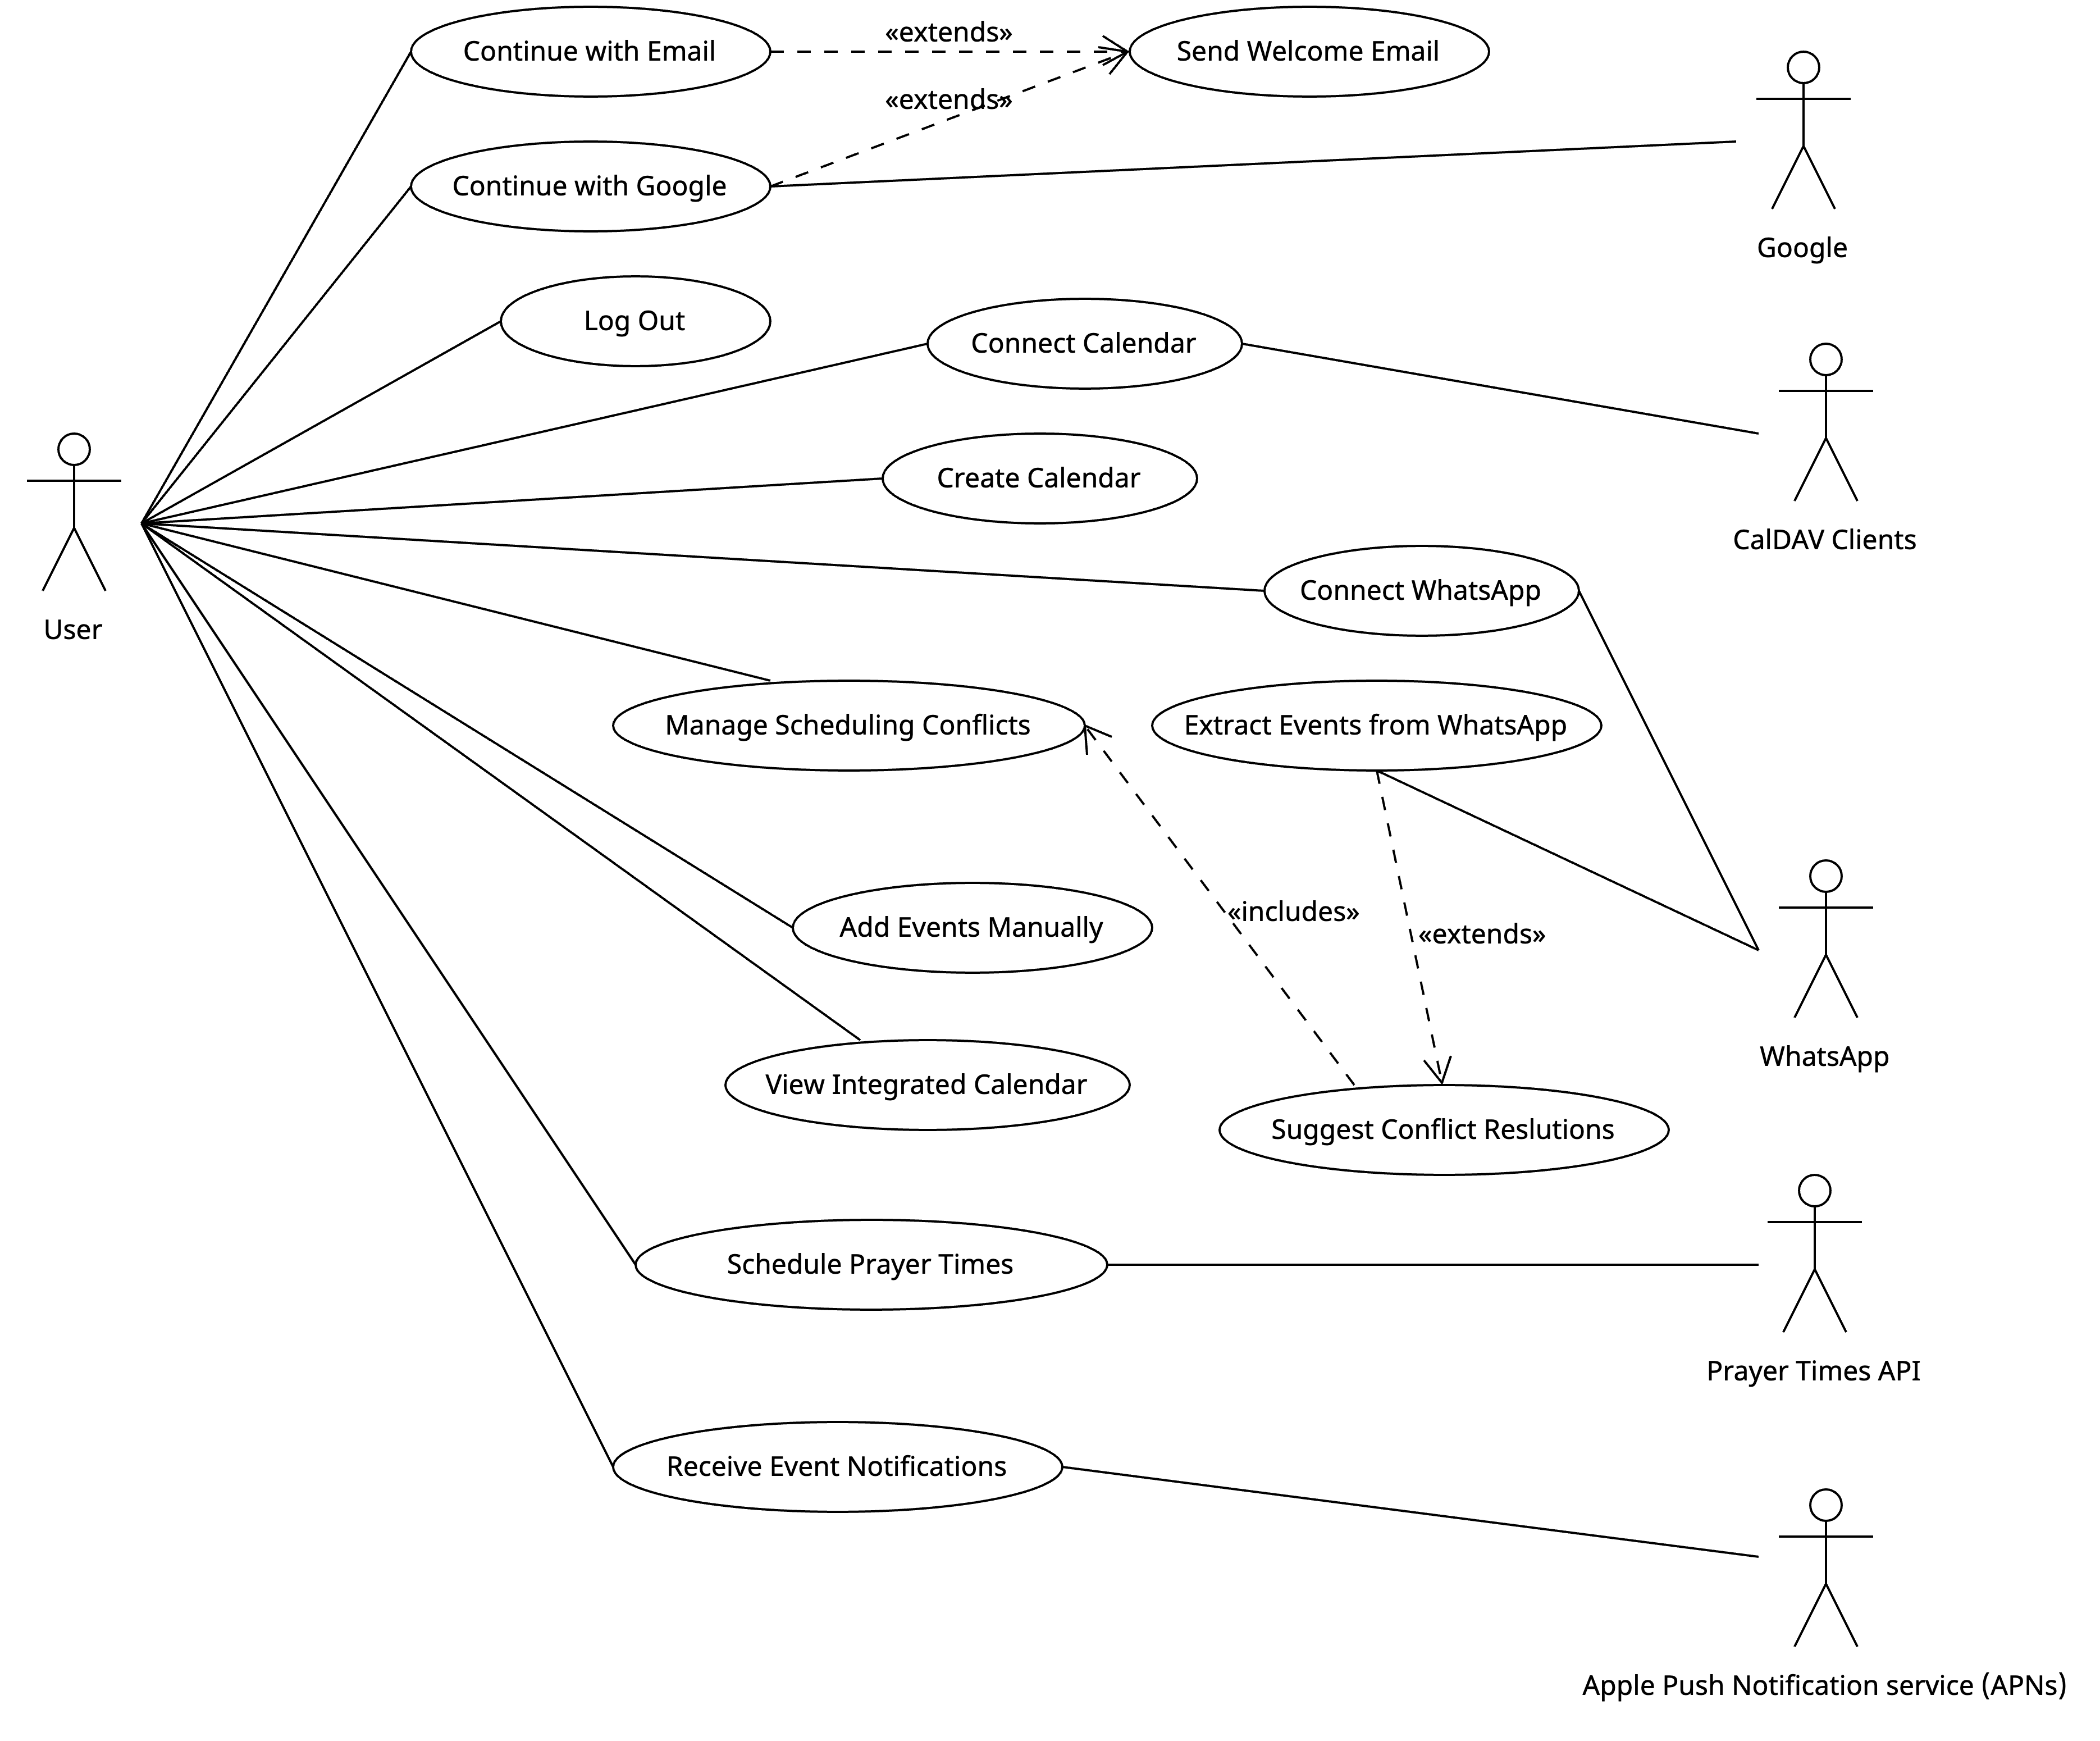
\includegraphics[width=\textwidth]{images/use-case-diagram.png}
    \caption{Use Case Diagram of Jadwal}
    \label{fig:use-case-diagram}
\end{figure}



\begin{usecase}{Continue with Email}
  \ucbasicinfo{High}{Regular}
  \ucshortdescription{This UC allows users to login or create an account using their email.}
  \uctrigger{This UC starts when the user enters their email to the system.}
  \ucactors{User}{None}
  \ucpreconditions{User must have an email}
  \ucrelationships{Send Welcome Email}{N/A}{N/A}
  \ucinputsoutputs{
    \begin{itemize}
      \item \textbf{Email} (Source: User)
      \item \textbf{Magic Link (from email)} (Source: User)
    \end{itemize}
  }{
    \begin{itemize}
      \item \textbf{Magic link email} (Destination: User)
      \item \textbf{Confirmation messages} (Destination: User Interface)
      \item \textbf{JWT} (Destination: App)
    \end{itemize}
  }
  \ucmainflow{
    \begin{enumerate}
      \item The user enters their email.
            \ucinfo{System displays an email input field.}
      \item System creates an account if the user has no account, and then generates and sends the magic link.
            \ucinfo{App displays ``Check your email'' message.}
      \item The user clicks the magic link in the email.
            \ucinfo{The app is opened on the device of the user.}
      \item The app sends the token to the system to log the user in.
            \ucinfo{System verifies token and logs user in.}
    \end{enumerate}
  }
  \ucalternateflows{
    \begin{itemize}
      \item The user cancels the authentication request.
    \end{itemize}
  }
  \ucexceptions{
    \begin{itemize}
      \item Invalid email format.
      \item Magic link token expired or invalid.
      \item \textbf{Request sending failure}: If sending the request fails due to network issues, the system prompts the user to try again.
    \end{itemize}
  }
  \ucconclusion{This UC ends when the user is logged in.}
  \ucpostconditions{The system generates a JWT.}
  \ucspecialrequirements{An email server must be present to send magic link email.}
\end{usecase}

\begin{figure}[!h]
  \centering
  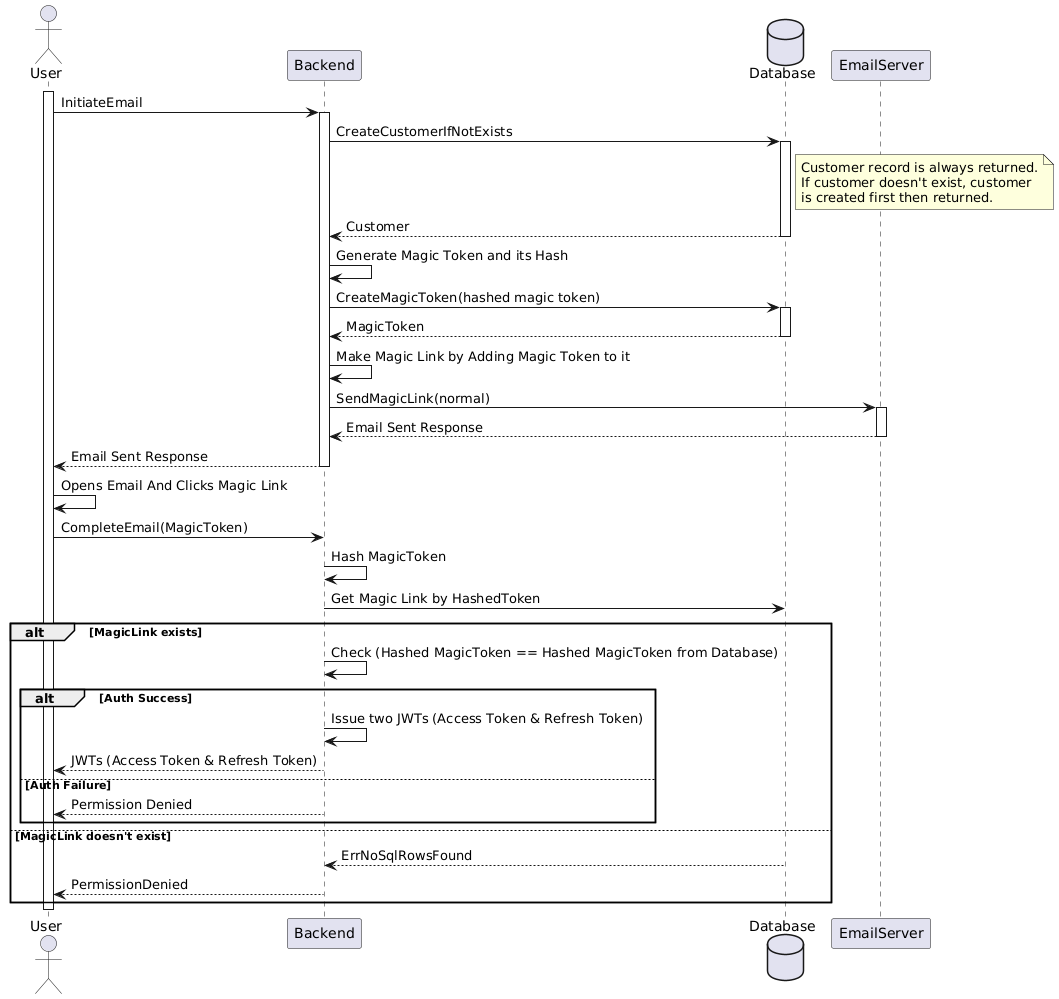
\includegraphics[width=\textwidth]{images/docs/diagrams/sequence-diagrams/all-sequence-diagrams/Continue with Email.png}
  \caption{Continue with Email Sequence Diagram}
  \label{fig:seq/continue-with-email}
\end{figure}

The "Continue with Email Sequence Diagram", shown in \textbf{Figure~\ref{fig:seq/continue-with-email}}, illustrates the process of email-based magic link authentication, involving interactions between the User, Backend, Database, and EmailServer. The process begins when the user initiates an action, such as signing up or logging in. The backend executes the CreateCustomerIfNotExists function to retrieve an existing customer record or create a new one if none exists. Once the customer is identified, the backend generates a magic token and its hashed version using the GenerateMagicToken function. The hashed token is stored in the database, and a magic link containing the token is created. The backend then sends the magic link to the user's email using the SendEmail function via the email server. The user clicks the magic link, triggering the CompleteFlow(MagicToken) request to the backend, where the provided token is validated against the stored hashed token in the database. If the tokens match, authentication succeeds, and the backend issues a JSON Web Token (JWT) to the user for future access. In cases where the token is invalid, expired, or the customer record is missing, the system responds with appropriate errors, such as PermissionDenied or EntryNotFound. This diagram demonstrates a secure flow for handling authentication via email magic links.
\begin{usecase}{Continue with Google}
  \ucbasicinfo{High}{Regular}
  \ucshortdescription{This UC allows users to login or sign up with their Google account.}
  \uctrigger{This UC starts when the user clicks ``Continue with Google'' button in the app.}
  \ucactors{User}{Google}
  \ucpreconditions{The user must have an active Google account.}
  \ucrelationships{Send Welcome Email}{N/A}{N/A}
  \ucinputsoutputs{
    \begin{itemize}
      \item \textbf{Google access token} (Source: User)
    \end{itemize}
  }{
    \begin{itemize}
      \item \textbf{Authentication response} (Destination: User)
      \item \textbf{JWT} (Destination: App)
    \end{itemize}
  }
  \ucmainflow{
    \begin{enumerate}
      \item The user click continue with Google.
        \ucinfo{App uses OAuth to authenticate with Google}
      \item App sends Google access token to the system.
        \ucinfo{System verifies the token is issued for us and then issues JWT for usage within the app.}
    \end{enumerate}
  }
  \ucalternateflows{
    \begin{itemize}
      \item The user cancels the authentication request.
    \end{itemize}
  }
  \ucexceptions{
    \begin{itemize}
      \item Google access token invalid or expired.
      \item \textbf{Request sending failure}: If sending the request fails due to network issues, the system prompts the user to try again.
    \end{itemize}
  }
  \ucconclusion{This UC ends when the user is logged in.}
  \ucpostconditions{The system generates a JWT.}
  \ucspecialrequirements{A google client must be present for the validation of the access token to be possible.}
\end{usecase}

\begin{figure}[!h]
  \centering
  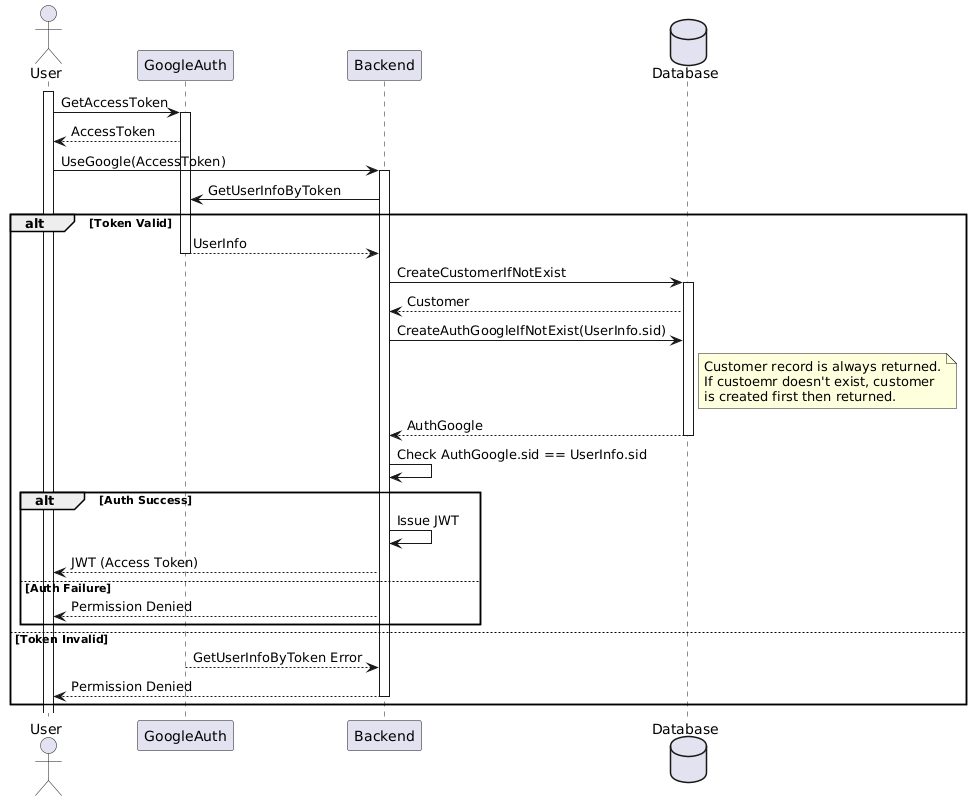
\includegraphics[width=\textwidth]{images/docs/diagrams/sequence-diagrams/all-sequence-diagrams/Continue with Google.png}
  \caption{Continue with Google Sequence Diagram}
  \label{fig:seq/continue-with-google}
\end{figure}
\begin{usecase}{Send Welcome Email}
    \ucbasicinfo{Low}{Regular}
    \ucshortdescription{This UC welcomes the user to the platform.}
    \uctrigger{This UC starts when the user account is created.}
    \ucactors{User}{None}
    \ucpreconditions{User account must be created in the system.}
    \ucrelationships{N/A}{N/A}{N/A}
    \ucinputsoutputs{
      \begin{itemize}
        \item \textbf{User name} (Source: System)
        \item \textbf{Welcome email template} (Source: System)
      \end{itemize}
    }{
      \begin{itemize}
        \item \textbf{Welcome email} (Destination: User)
      \end{itemize}
    }
    \ucmainflow{
      \begin{enumerate}
        \item The system fetches the user information.
          \ucinfo{The database is used.}
        \item The system fetches the send welcome email template.
          \ucinfo{The template is filled with the user name.}
        \item The system sends the email with the template.
          \ucinfo{The email is received by the user welcoming them.}
      \end{enumerate}
    }
    \ucexceptions{
      \begin{itemize}
        \item Email server is down.
      \end{itemize}
    }
    \ucconclusion{This UC ends when the user receives an email from us welcoming them.}
    \ucspecialrequirements{An email server must be present to send welcome email.}
\end{usecase}

\begin{figure}[!h]
  \centering
  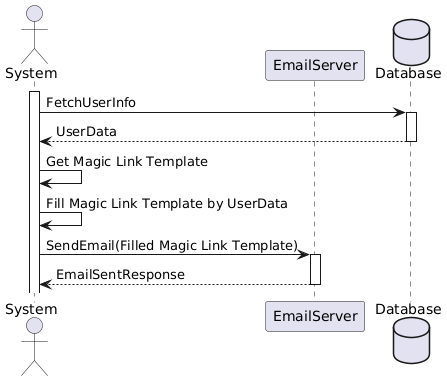
\includegraphics[width=\textwidth]{images/docs/diagrams/sequence-diagrams/all-sequence-diagrams/Send Welcome Email.png}
  \caption{Send Welcome Email Sequence Diagram}
  \label{fig:seq/send-welcome-email}
\end{figure}
\begin{usecase}{Continue with Google}
  \ucbasicinfo{\#2}{HIGH}{Regular}
  \ucshortdescription{This UC allows users to login or continue with Google if we have a Google account}
  \uctrigger{This UC starts when the user enters their email to the system.}
  \ucactors{User}{Google}
  \ucpreconditions{User must have an activated or valid Google email.}
  \ucrelationships{Send Welcome Email}{N/A}{N/A}
  \ucinputsoutputs{
    \begin{itemize}
      \item \textbf{Google account} (Source: User)
      \item \textbf{Authentication request to Google} (Source: System)
    \end{itemize}
  }{
    \begin{itemize}
      \item \textbf{Success or error message} (Destination: User)
      \item \textbf{Authentication response} (Destination: Google)
    \end{itemize}
  }
  \ucmainflow{
    \begin{enumerate}
      \item The user click continue with Google.
        \ucinfo{System displays "continue with Google" button}
      \item Authentication request.
        \ucinfo{A request sent to Google for user authentication and get JWT and sent it to the system, while the system will generate a our JWT}
      \item Authentication response.
        \ucinfo{Confirmation of successful authentication}
    \end{enumerate}
  }
  \ucalternateflows{
    \begin{itemize}
      \item User cancels authentication
      \item Authentication failure
    \end{itemize}
  }
  \ucexceptions{
    \begin{itemize}
      \item Invalid Google email
      \item Network issue
    \end{itemize}
  }
  \ucconclusion{}
  \ucpostconditions{The user is successfully authenticated and redirected to the main application interface}
  \ucbusinessrules{
    \begin{itemize}
      \item User should have valid Google account
    \end{itemize}
  }
  \ucspecialrequirements{Sign-in page should display clear button and error message}
\end{usecase}
\begin{usecase}{Connect Calendar}
    \ucbasicinfo{Medium}{Regular}
    \ucshortdescription{This UC allows the user to access their iOS device calendars through EventKit and configure CalDAV accounts.}
    \uctrigger{This UC is triggered when the user first launches the app or manually initiates calendar access.}
    \ucactors{User}{EventKit}
    \ucpreconditions{User must be logged in}
    \ucrelationships{N/A}{N/A}{N/A}
    \ucinputsoutputs{
        \begin{itemize}
            \item \textbf{Calendar Access Permission} (Source: User)
            \item \textbf{CalDAV Account Credentials} (Source: Backend)
        \end{itemize}
    }{
        \begin{itemize}
            \item \textbf{Local Calendar Access Status} (Destination: System)
            \item \textbf{Calendar Events} (Destination: App)
        \end{itemize}
    }
    \ucmainflow{
        \begin{enumerate}
            \item The system requests calendar access permission from the user.
                  \ucinfo{The app requests EventKit authorization to access device calendars.}
            \item The system retrieves CalDAV account credentials from the backend.
                  \ucinfo{The app fetches encrypted credentials for our CalDAV server.}
            \item The system configures CalDAV accounts through iOS's native calendar system.
                  \ucinfo{EventKit handles direct communication with all CalDAV servers (both ours and external ones).}
            \item The system fetches calendar events using EventKit.
                  \ucinfo{Events are fetched from all configured calendar accounts through iOS's native calendar system.}
            \item The system sets up local notifications for calendar events.
                  \ucinfo{Notifications are scheduled locally based on event reminders.}
        \end{enumerate}
    }
    \ucalternateflows{
        \begin{enumerate}
            \item If calendar access is denied, the user can grant permission through device settings.
            \item If account configuration fails, the user can retry the connection through iOS settings.
        \end{enumerate}
    }
    \ucexceptions{
        \begin{itemize}
            \item Calendar access permission denied
            \item Network issue retrieving account credentials
            \item iOS calendar account configuration failure
        \end{itemize}
    }
    \ucconclusion{The UC ends when the user has access to their device calendars and CalDAV accounts are configured in iOS.}
    \ucpostconditions{The app can read calendar events through EventKit from all configured calendar sources.}
    \ucspecialrequirements{The system must rely on iOS's native calendar system for all CalDAV communication.}
\end{usecase}

\begin{figure}[!h]
    \centering
    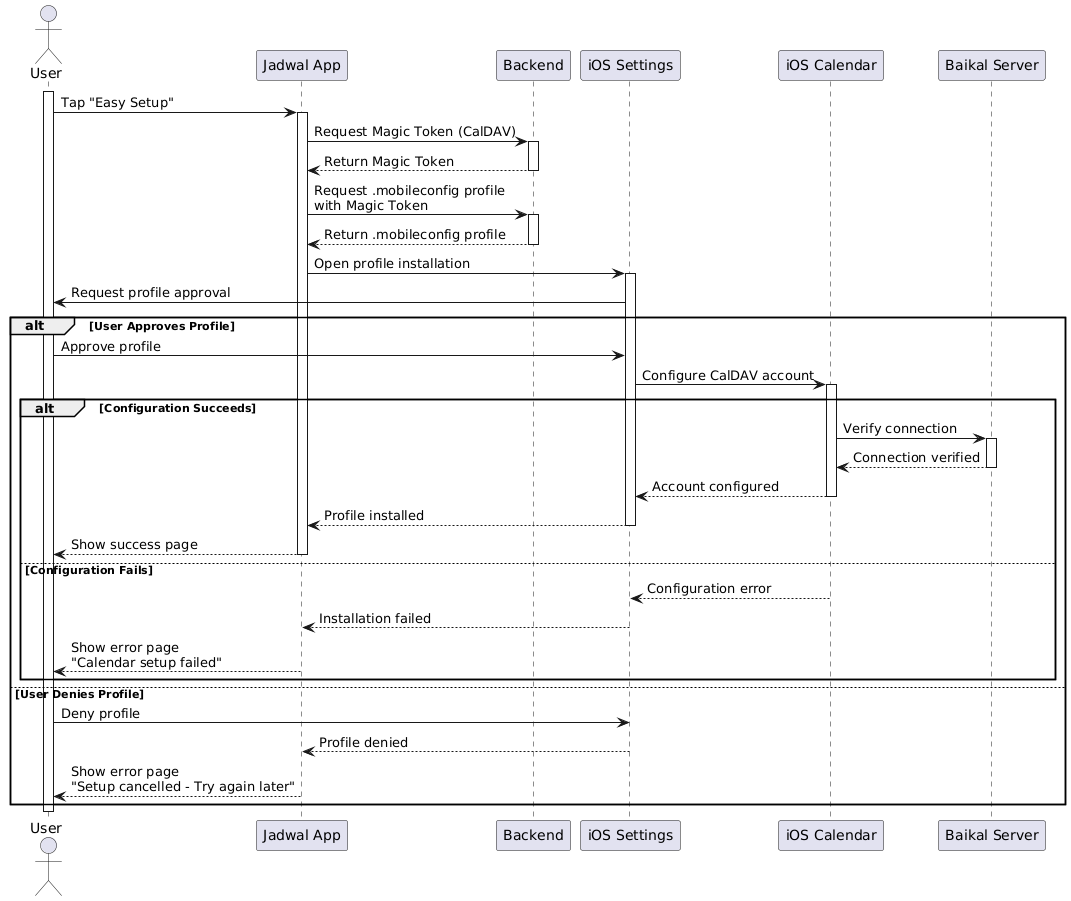
\includegraphics[width=\textwidth]{images/docs/diagrams/sequence-diagrams/all-sequence-diagrams/Connect Calendar.png}
    \caption{Connect Calendar Sequence Diagram}
    \label{fig:seq/connect-calendar}
\end{figure}

The ``Connect Calendar Sequence Diagram'', shown in \textbf{Figure~\ref{fig:seq/connect-calendar}}, illustrates the calendar integration process:

\begin{enumerate}
    \item \textbf{Local Calendar Access:} The iOS app uses EventKit framework to request and manage access to the device's calendars. This provides direct access to the user's existing calendar data.

    \item \textbf{Account Configuration:} The app retrieves encrypted CalDAV account credentials from the backend and uses iOS's native calendar system to configure the accounts. EventKit and iOS handle all direct communication with CalDAV servers, both our own and external ones.
\end{enumerate}

The Backend's role is strictly limited to securely storing and providing encrypted CalDAV account credentials. All calendar data synchronization, CalDAV communication, and event management happens through iOS's native calendar system using EventKit. This approach leverages iOS's built-in CalDAV client capabilities, ensuring reliable calendar synchronization while maintaining security of sensitive credentials.
\begin{usecase}{Create Calendar}
  \ucbasicinfo{High}{Regular}
  \ucshortdescription{This UC allows the user to create a new calendar using iOS EventKit.}
  \uctrigger{This UC is triggered when the user clicks ``Create Calendar'' in the app.}
  \ucactors{User}{EventKit}
  \ucpreconditions{
    \begin{itemize}
      \item User must be logged in
      \item Calendar access must be authorized in iOS Settings
      \item Baikal CalDAV account must be configured
    \end{itemize}
  }
  \ucrelationships{N/A}{N/A}{N/A}
  \ucinputsoutputs{
    \begin{itemize}
      \item \textbf{Calendar name} (Source: User)
      \item \textbf{Calendar account to add calendar under} (Source: User)
      \item \textbf{Calendar color} (Source: User)
    \end{itemize}
  }{
    \begin{itemize}
      \item \textbf{New calendar} (Destination: EventKit)
      \item \textbf{Creation status} (Destination: App)
    \end{itemize}
  }
  \ucmainflow{
    \begin{enumerate}
      \item The user taps the ``Calendar'' icon button in the app toolbar in the ``Calendar'' screen.
            \ucinfo{The app presents a ``Calendars'' sheet.}
      \item The user clicks the ``plus'' icon button in the toolbar of the ``Calendars'' sheet.
            \ucinfo{The app presents a form for calendar name, selector to choose account to add calendar under, and calendar color.}
      \item The user enters calendar name, selects a color, and selector to choose account to add calender under.
            \ucinfo{The app uses EventKit to create a new calendar.}
      \item EventKit creates the calendar and handles synchronization.
            \ucinfo{The calendar appears in the user's calendar list.}
    \end{enumerate}
  }
  \ucalternateflows{
    \begin{itemize}
      \item If calendar creation fails, the app shows an error and allows retry.
    \end{itemize}
  }
  \ucexceptions{
    \begin{itemize}
      \item \textbf{EventKit access denied:} The app prompts to enable calendar access in Settings.
      \item \textbf{Network issues:} EventKit handles synchronization internally.
    \end{itemize}
  }
  \ucconclusion{The UC ends when EventKit confirms the calendar creation.}
  \ucpostconditions{A new calendar is created through EventKit.}
  \ucspecialrequirements{The system must use EventKit for all calendar operations.}
\end{usecase}

\begin{figure}[!h]
  \centering
  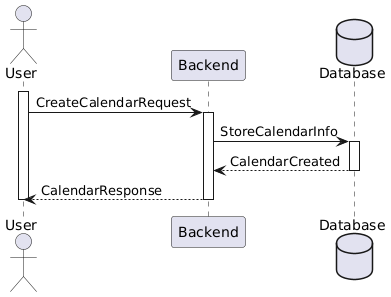
\includegraphics[width=0.5\textwidth]{images/docs/diagrams/sequence-diagrams/all-sequence-diagrams/Create Calendar.png}
  \caption{Create Calendar Sequence Diagram}
  \label{fig:seq/create-calendar}
\end{figure}

The ``Create Calendar Sequence Diagram'', shown in \textbf{Figure~\ref{fig:seq/create-calendar}}, illustrates the process of creating a new calendar in the Jadwal app. The sequence begins when the user accesses the calendar creation interface through the ``Calendars'' sheet, accessed via the calendar icon in the toolbar.

The flow involves several key steps:
\begin{enumerate}
  \item The user provides essential calendar details through a form interface:
        \begin{itemize}
          \item Calendar name
          \item Account selection (where to add the calendar)
          \item Calendar color
        \end{itemize}
  \item The app communicates with EventKit to create the new calendar
  \item EventKit handles the calendar creation and all necessary synchronization
\end{enumerate}

The process is designed to be robust and user-friendly:
\begin{itemize}
  \item If EventKit access is denied, the app guides users to enable calendar access in iOS Settings
  \item If creation fails, the app shows an error and allows retry
  \item EventKit handles all synchronization internally
\end{itemize}

This implementation leverages iOS's native EventKit framework, which manages all calendar operations and synchronization internally. This provides a reliable and native iOS experience while ensuring proper calendar management.
\begin{usecase}{Connect WhatsApp}
  \ucbasicinfo{Medium}{Regular}
  \ucshortdescription{This UC allows the user to connect their WhatsApp account to the system.}
  \uctrigger{This UC is triggered when the user clicks on ``Connect WhatsApp'' button in the app.}
  \ucactors{User}{WhatsApp}
  \ucpreconditions{User must be logged in}
  \ucrelationships{N/A}{N/A}{N/A}
  \ucinputsoutputs{
    \begin{itemize}
      \item \textbf{WhatsApp phone number} (Source: User)
      \item \textbf{WhatsApp linking code} (Source: User)
    \end{itemize}
  }{
    \begin{itemize}
      \item \textbf{WhatsApp auth credentials} (Destination: System)
    \end{itemize}
  }
  \ucmainflow{
    \begin{enumerate}
      \item The user clicks ``Connect WhatsApp'' button.
            \ucinfo{The system asks for the user's WhatsApp phone number.}
      \item The user enters their WhatsApp phone number.
            \ucinfo{WhatsApp shows the linking code in their app.}
      \item The user enters the linking code in our app.
            \ucinfo{The app shows a success screen if connection was sucessful.}
    \end{enumerate}
  }
  \ucalternateflows{
    \begin{itemize}
      \item If the WhatsApp connection fails, the user must redo the steps and try again.
      \item If the user enters a wrong linking code, the connection of the WhatsApp account will fail unless they enter the correct code.
    \end{itemize}
  }
  \ucexceptions{
    \begin{itemize}
      \item \textbf{Wrong linking code:} If the user enters a wrong linking code too many times, the connection of the WhatsApp account will fail.
      \item \textbf{Network issue:} A network issue interrupting the communication between the app, the server, and WhatsApp.
    \end{itemize}
  }
  \ucconclusion{The UC ends when the user has a connected WhatsApp account in the system.}
  \ucpostconditions{The system has access to the user's WhatsApp account.}
\end{usecase}

\begin{figure}[!h]
  \centering
  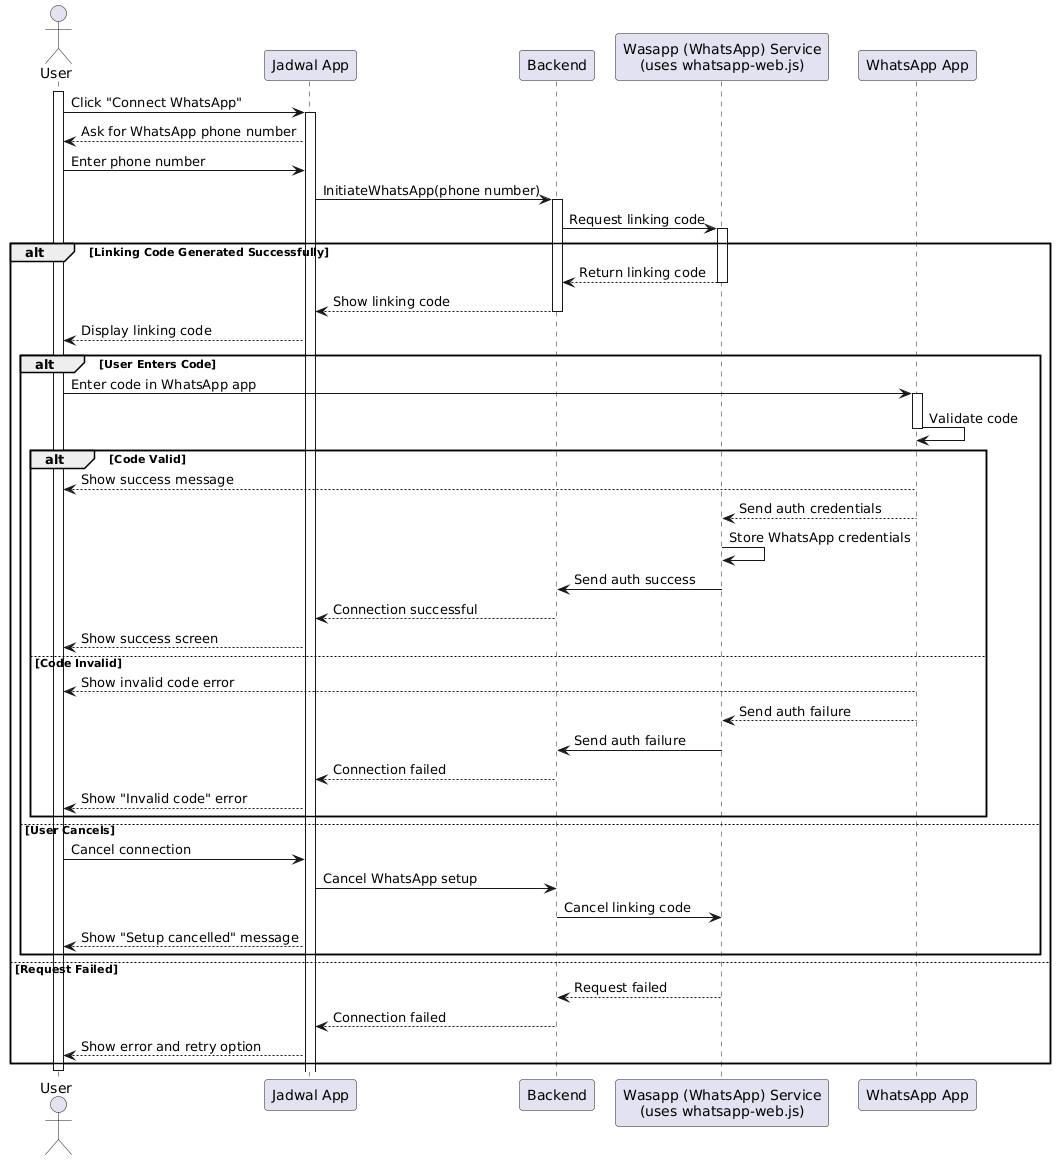
\includegraphics[width=\textwidth]{images/docs/diagrams/sequence-diagrams/all-sequence-diagrams/Connect WhatsApp.png}
  \caption{Connect WhatsApp Sequence Diagram}
  \label{fig:seq/connect-whatsapp}
\end{figure}

The "Connect WhatsApp Sequence Diagram", shown in \textbf{Figure~\ref{fig:seq/connect-whatsapp}}, illustrates the two-phase authentication process for connecting a user's WhatsApp account to Jadwal. The sequence begins with the InitiateWhatsApp gRPC call, where the user provides their phone number to the Backend.

The Backend then communicates with the WhatsApp service to request a linking code. This interaction follows two possible paths:

\begin{itemize}
  \item If the linking code request succeeds:
        \begin{enumerate}
          \item The user receives the linking code in their WhatsApp application
          \item The user initiates the CompleteWhatsApp gRPC call with the linking code
          \item The Backend validates the code with WhatsApp
          \item Upon successful validation, the WhatsApp authentication credentials are securely stored in the Database for future use
        \end{enumerate}
  \item If the linking code request fails:
        \begin{itemize}
          \item The Backend immediately returns an InitiateWhatsApp failure response to the user
        \end{itemize}
\end{itemize}

During the completion phase, if the linking code validation fails, the Backend returns a CompleteWhatsApp failure response, requiring the user to restart the process. This secure two-phase authentication ensures that only legitimate WhatsApp account owners can connect their accounts to Jadwal while maintaining the integrity of the WhatsApp integration.
\begin{usecase}{Extract Events from WhatsApp}
  \ucbasicinfo{High}{Regular}
  \ucshortdescription{Allows users to extract event details shared in WhatsApp messages and save them to their calendar.}
  \uctrigger{User selects a message containing event details in WhatsApp.}
  \ucactors{User}{WhatsApp}
  \ucpreconditions{User must have WhatsApp installed and linked to the system.}
  \ucrelationships{N/A}{Event Management}{N/A}
  \ucinputsoutputs{
    \begin{itemize}
      \item \textbf{User-selected WhatsApp message containing event details.} (Source: User)
    \end{itemize}
  }{
    \begin{itemize}
      \item \textbf{Extracted event details saved to the calendar.} (Destination: User)
    \end{itemize}
  }
  \ucmainflow{
    \begin{enumerate}
      \item User opens WhatsApp and selects a message with event details. 
        \ucinfo{Display of the selected message.}
      \item User taps on the ``Extract Event'' option.
        \ucinfo{System processes the message to identify event details.}
      \item System extracts event details from the message.
        \ucinfo{Date, time, and location are parsed from the text. }
    \end{enumerate}
  }
  \ucalternateflows{
    \begin{itemize}
      \item If the message does not contain valid event details, display an error message.
      \item Notify the user about invalid format. 
    \end{itemize}
  }
  \ucexceptions{
    \begin{itemize}
      \item If there is a system error during extraction, display a relevant error message. 
      \item Log error for troubleshooting.
    \end{itemize}
  }
  \ucconclusion{User successfully extracts event details from WhatsApp and saves them to the calendar.}
  \ucpostconditions{The event is added to the user's calendar, and the user can view it in their schedule.}
  \ucbusinessrules{
    \begin{itemize}
      \item Only messages with recognized event formats can be extracted.
    \end{itemize}
  }
  \ucspecialrequirements{The system must have permissions to access WhatsApp messages and extract relevant information.}
\end{usecase}
\begin{usecase}{Suggest Conflict Resolutions}
  \ucbasicinfo{HIGH}{Regular}
  \ucshortdescription{This UC gives the user all the conflicts and possible ways to resolve it.}
  \uctrigger{The UC is triggered when a conflict is detected between any overlapping event}
  \ucactors{User}{Calendar System, WhatsApp}
  \ucpreconditions{The calendar must have events}
  \ucrelationships{None}{Manage Scheduling Conflicts}{None}
  \ucinputsoutputs{
    \begin{itemize}
      \item Overlapping events (Source: User or WhatsApp extraction)
      \item User suggested resolution (Source: User)
    \end{itemize}
  }{
    \begin{itemize}
      \item {Resolution options} (Destination: User Interface)
      \item {Updated calendar schedule} (Destination: Calendar)
    \end{itemize}
  }
  \ucmainflow{
    \begin{enumerate}
      \item Conflict Detection  
        \ucinfo{The system detects overlapping of events either added manually or extracted from WhatsApp.}
      \item Offer Resolutions
        \ucinfo{The system provides the user with the list of resolution options.
        \begin{itemize}
          \item By moving the overlapping event to another time slot.   
          \item Keep both events with a conflict warning. 
        \end{itemize}}
      \item User Selection  
        \ucinfo{The user moves the overlapping event to another time slot by the list provided by the system}
      \item Implement Resolution
        \ucinfo{The system makes the changes in the calendar respectively}
    \end{enumerate}
  }
  \ucalternateflows{
    \begin{enumerate}
      \item {N/A}
    \end{enumerate}
  }
  \ucexceptions{
    \begin{itemize}
      \item If the system doesn't get any possible way to resolve the conflict then the system would mark both the event as conflicting or displays to delete one of the event.
      \item If the user doesn't choose any option to resolve the conflict then both the events are makrd as conflicting.
    \end{itemize}
  }
  \ucconclusion{The UC ends when the user gives it's input for resolution weather if it's to reschedule the event, delete it or leave it without resolving and it is reflected in on the calendar.}
  \ucpostconditions{The conflicting events in the calendar are either resolved or marked as conflicting}
  \ucspecialrequirements{The system give feasible conflict resolution options}
\end{usecase}

\begin{usecase}{Manage Scheduling Conflicts}
  \ucbasicinfo{Medium}{Regular}
  \ucshortdescription{This UC allows the user to manage scheduling conflicts by suggesting resolutions when overlapping events are detected.}
  \uctrigger{This UC is triggered when an automatically added event overlaps with an existing event.}
  \ucactors{User}{None}
  \ucpreconditions{
    \begin{itemize}
      \item User is logged in.
      \item Conflicting events list is not empty.
    \end{itemize}
  }
  \ucrelationships{N/A}{N/A}{N/A}
  \ucinputsoutputs{
    \begin{itemize}
      \item \textbf{Conflicting events} (Source: System)
      \item \textbf{Event to override} (Source: User)
    \end{itemize}
  }{
    \begin{itemize}
      \item \textbf{Conflict resolution suggestion} (Destination: User Interface)
      \item \textbf{Updated event schedules} (Destination: Calendar)
    \end{itemize}
  }
  \ucmainflow{
    \begin{enumerate}
      \item The user opens the application and clicks on the view conflicts icon
        \ucinfo{The application shows all the conflics with their resolution options}
      \item The user chooses the best fit option to manage each conflict 
        \ucinfo{The conflict is resolved and is removed from the conflict list }

    \end{enumerate}
  }
  \ucalternateflows{
    \begin{enumerate}
      \item If the user doesn't choose any option, it shows conflicting status until the user chooses any option or the event expires. 
      \item If the user clicks on reject the event is left overlapping.
    \end{enumerate}
  }
  \ucexceptions{
    \begin{itemize}
      \item Netwok failure 
    \end{itemize}
  }
  \ucconclusion{The UC ends when the conflicting events are either resolved or marked as conflicting, based on the user's choice.}
  \ucpostconditions{The calendar reflects the user's decision regarding event conflicts.}
  \ucspecialrequirements{The system should provide best suggestions for resolving conflicts.}
\end{usecase}

\begin{figure}[!h]
  \centering
  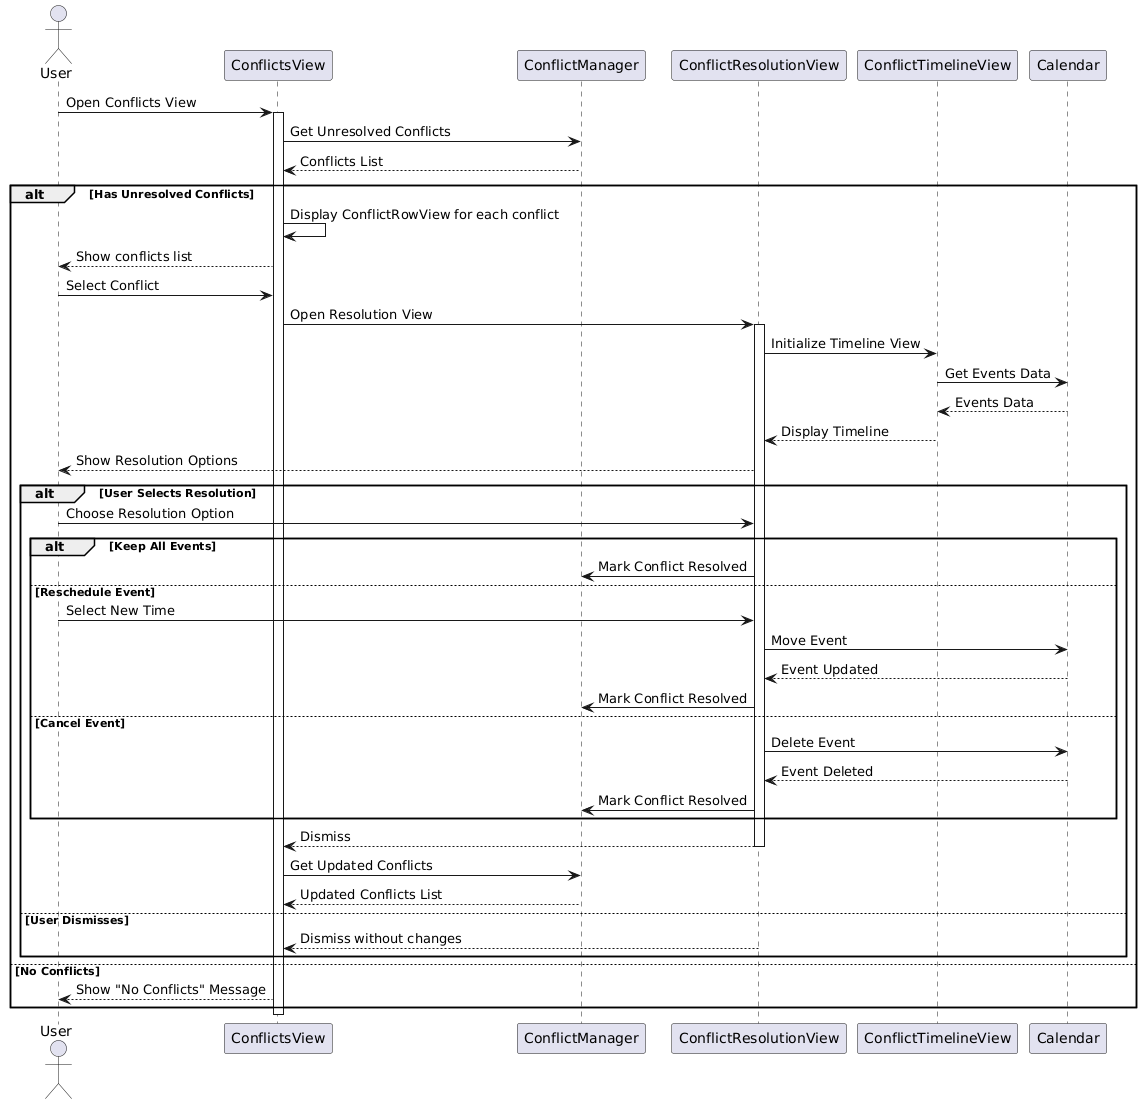
\includegraphics[width=\textwidth]{images/docs/diagrams/sequence-diagrams/all-sequence-diagrams/Manage Scheduling Conflicts.png}
  \caption{Manage Scheduling Conflicts Sequence Diagram}
  \label{fig:seq/manage-scheduling-conflicts}
\end{figure}
\begin{usecase}{Add Event Manually}
    \ucbasicinfo{High}{Regular}
    \ucshortdescription{This UC allows users to add events manually }
    \uctrigger{The user clicks and adds the events.}
    \ucactors{User}{None}
    \ucpreconditions{The user is logged into the application }
    \ucrelationships{N/Al}{N/A}{N/A}
    \ucinputsoutputs{
      \begin{itemize}
        \item \textbf{Event Name} (Source: User)
        \item \textbf{Event Location} (Source: User)
        \item \textbf{Event Date (Start and End)} (Source: User)
        \item \textbf{Event Time (Start and End)} (Source: User)
        \item \textbf{Event Description} (Source: User)
        \item \textbf{Notifications/Reminders} (Source: User)
      \end{itemize}
    }{
      \begin{itemize}
        \item \textbf{The event is displayed on the calendar with its details and duration
        } (Destination: Calendar)
      \end{itemize}
    }
    \ucmainflow{
      \begin{enumerate}
        \item The name of the event (e.g., ``Meeting with Client'')
          \ucinfo{Event is saved and displayed on the user’s calendar}
        \item The start and end time of the event.
          \ucinfo{The system displays the event in the correct time slot with its duration, while checking for conflicts and scheduling notifications}
        \item The User optionally adds a description
          \ucinfo{The system stores and displays description of the event.}
        \item Set reminders for the event.
          \ucinfo{Notification or reminder set for the event}
      \end{enumerate}
    }
    \ucalternateflows{
      \begin{enumerate}
        \item User clicks on a date on the calendar to bring up a popup with event fields and the date is pre-filled. 
        \item	The user can add a different color for the events.
      \end{enumerate}
    }
    \ucexceptions{
      \begin{itemize}
        \item Invalid date and time format\
        \item The event's start and end times conflict with an existing event
        \item The user attempts to save the event without filling in mandatory fields
      \end{itemize}
    }
    \ucconclusion{The UC ends when the event has been successfully added to the calendar, and the user sees it displayed.}
    \ucpostconditions{The event is successfully added to the calendar, visible in the correct time slot, and notifications are set as per user preferences}
    \ucspecialrequirements{The interface must be simple and allowing users to input events with less efforts.}
\end{usecase}
\begin{usecase}{View Integrated Calendar}
  \ucbasicinfo{High}{Regular}
  \ucshortdescription{Allows users to view their integrated calendar}
  \uctrigger{User selects the option to view the integrated calendar.}
  \ucactors{User}{None}
  \ucpreconditions{User must be logged into the system.}
  \ucrelationships{N/A}{N/A}{N/A}
  \ucinputsoutputs{
    \begin{itemize}
      \item \textbf{Integrated calendar} (Source: System)
    \end{itemize}
  }{
    \begin{itemize}
      \item \textbf{Integrated calendar} (Destination: App)
    \end{itemize}
  }
  \ucmainflow{
    \begin{enumerate}
      \item The user clicks on the integrated calendar.
            \ucinfo{The system displays the all integrated calendars and it's events}
    \end{enumerate}
  }
  \ucconclusion{User successfully views their integrated calendar with all the events.}
  \ucpostconditions{The integrated calendar is displayed}
  \ucspecialrequirements{N/A}
  \ucbusinessrules{
    \begin{itemize}
      \item \textbf{Events must be displayed according to user preferences .}
    \end{itemize}
  }
\end{usecase}

\begin{figure}[!h]
  \centering
  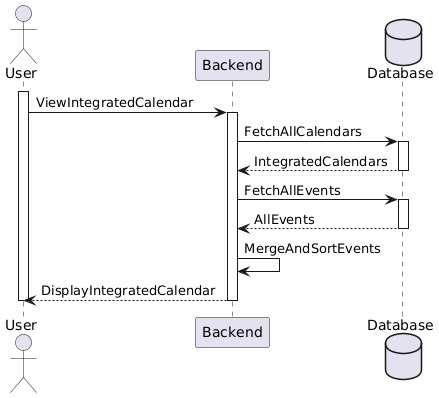
\includegraphics[width=\textwidth]{images/docs/diagrams/sequence-diagrams/all-sequence-diagrams/View Integrated Calendar.png}
  \caption{View Integrated Calendar Sequence Diagram}
  \label{fig:seq/view-integrated-calendar}
\end{figure}

The "View Integrated Calendar Sequence Diagram", shown in \textbf{Figure~\ref{fig:seq/view-integrated-calendar}}, demonstrates the process of presenting a unified view of all connected calendars to the user. The sequence begins when the user initiates a ViewIntegratedCalendar gRPC call to access their comprehensive calendar view.

The Backend executes a two-phase data retrieval process:
\begin{enumerate}
  \item First queries the Database via FetchAllCalendars to retrieve all calendar sources connected to the user's account
  \item Then executes FetchAllEvents to gather events from all calendars
\end{enumerate}

After data retrieval, the Backend performs critical processing:
\begin{itemize}
  \item Merges events from different calendar sources
  \item Sorts events chronologically
  \item Applies user preferences for event display
\end{itemize}

Finally, the Backend returns the processed calendar data through the gRPC channel as DisplayIntegratedCalendar response. This unified view ensures users can efficiently manage their schedule across all connected calendars, maintaining consistency with user preferences while providing a comprehensive overview of all commitments.
\begin{usecase}{Schedule Prayer Times}
    \ucbasicinfo{High}{Regular}
    \ucshortdescription{Allows users to create, edit, and manage their prayer time schedules.}
    \uctrigger{User selects the option to schedule prayer times.}
    \ucactors{User}{None}
    \ucpreconditions{User must be logged into the system.}
    \ucrelationships{N/A}{N/A}{N/A}
    \ucinputsoutputs{
      \begin{itemize}
        \item \textbf{User's prayer time details} (Source: user)
        \item \textbf{(date, time)}
      \end{itemize}
    }{
      \begin{itemize}
        \item \textbf{Confirmation of scheduled prayer times, calendar entries.}
      \end{itemize}
    }
    \ucmainflow{
      \begin{enumerate}
        \item User navigates to the prayer scheduling page.
          \ucinfo{User is presented with a form to enter prayer times. Display of the scheduling interface.}
        \item User inputs prayer time details.
          \ucinfo{Input fields for time, date, and prayer type. User's input is captured for validation.}
        \item User saves the schedule.
          \ucinfo{System checks for valid input. Confirmation message displayed.}
        \item System confirms schedule creation.
          \ucinfo{User receives a notification. Scheduled prayer times are saved in the system.}
      \end{enumerate}
    }
    \ucalternateflows{
      \begin{itemize}
        \item If input is invalid, display error messages.
      \end{itemize}
    }
    \ucexceptions{
      \begin{itemize}
        \item If there's a system error, display a relevant error message.
      \end{itemize}
    }
    \ucpostconditions{The system generates calendar entries for the scheduled prayer times.}
    \ucspecialrequirements{The system must support notifications for prayer times.}
    \ucconclusion{User's prayer times are successfully scheduled.}
    \ucbusinessrules{
      \begin{itemize}
        \item Prayer times must be within valid time ranges.
      \end{itemize}
    }
\end{usecase}
\begin{usecase}{Receive Event Notifications}
  \ucbasicinfo{High}{Regular}
  \ucshortdescription{Users receive notifications about upcoming events.}
  \uctrigger{The UC is triggered when the choosen time of an event's reminder has arrived}
  \ucactors{User}{None}
  \ucpreconditions{User must be logged into the system and set a reminder of the specific event.}
  \ucrelationships{N/A}{N/A}{N/A}
  \ucinputsoutputs{
    \begin{itemize}
      \item \textbf{Time of the event reminder} (Source: User)
    \end{itemize}
  }{
    \begin{itemize}

      \item \textbf{Notifications sent to users.} (Destination: System)
    \end{itemize}
  }
  \ucmainflow{
    \begin{enumerate}
      \item The system checks the alarms set for every event.
            \ucinfo{The system checks every 1 minute for set alarms for every event.}
      \item Notifications sent to users.
            \ucinfo{The user is reminded about the event by sending the notification}
    \end{enumerate}
  }
  \ucalternateflows{
    \begin{itemize}
      \item \textbf{If user denys the access to the notification the notifications are not sent.}
    \end{itemize}
  }
  \ucexceptions{
    \begin{itemize}
      \item \textbf{Netwok issue}
    \end{itemize}
  }
  \ucconclusion{The system checks for set alarm every 1 minute and if the event is detected the system sends the notification.}
  \ucpostconditions{Notifications are sent.}
  \ucspecialrequirements{Notification permission.}
  \ucbusinessrules{The system has to check every minute for the set alarm.
  }
\end{usecase}

\begin{figure}[!h]
  \centering
  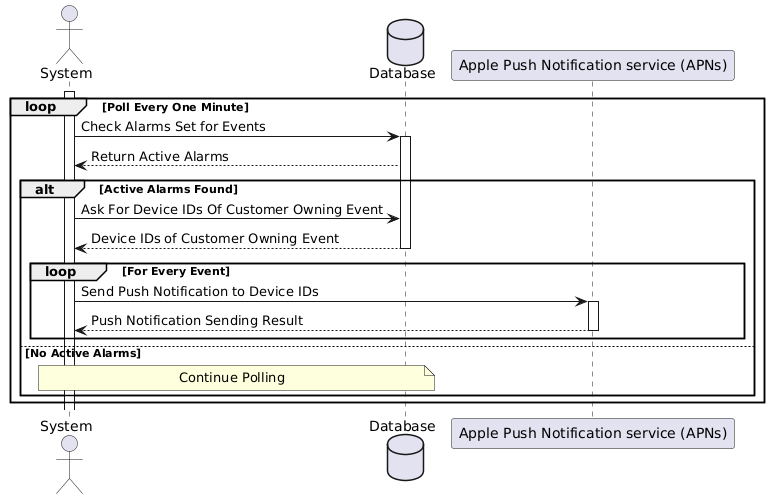
\includegraphics[width=\textwidth]{images/docs/diagrams/sequence-diagrams/all-sequence-diagrams/Receive Event Notifications.png}
  \caption{Receive Event Notifications Sequence Diagram}
  \label{fig:seq/receive-event-notifications}
\end{figure}

The ``Receive Event Notifications Sequence Diagram'', shown in \textbf{Figure~\ref{fig:seq/receive-event-notifications}}, illustrates Jadwal's continuous event notification monitoring and delivery system. The sequence operates in a continuous polling loop that executes every minute, ensuring timely notification delivery for all scheduled events.

The polling process consists of several key steps:
\begin{enumerate}
  \item The System queries the Database for active alarms through regular checks
  \item For each batch of active alarms found:
        \begin{itemize}
          \item Retrieves associated device IDs for notification targets
          \item Iterates through each event requiring notification
          \item Dispatches push notifications via Apple Push Notification service (APNs)
        \end{itemize}
  \item If no active alarms are found, the system continues its polling cycle
\end{enumerate}

This robust notification system ensures reliable delivery of event reminders while efficiently managing system resources. The one-minute polling interval provides a balance between timely notifications and system performance, while the batch processing of notifications optimizes the interaction with APNs. The system's ability to handle multiple device IDs per user ensures notifications reach users across all their registered devices.

\section{Activity Diagram}

\begin{figure}[!h]
    \centering
    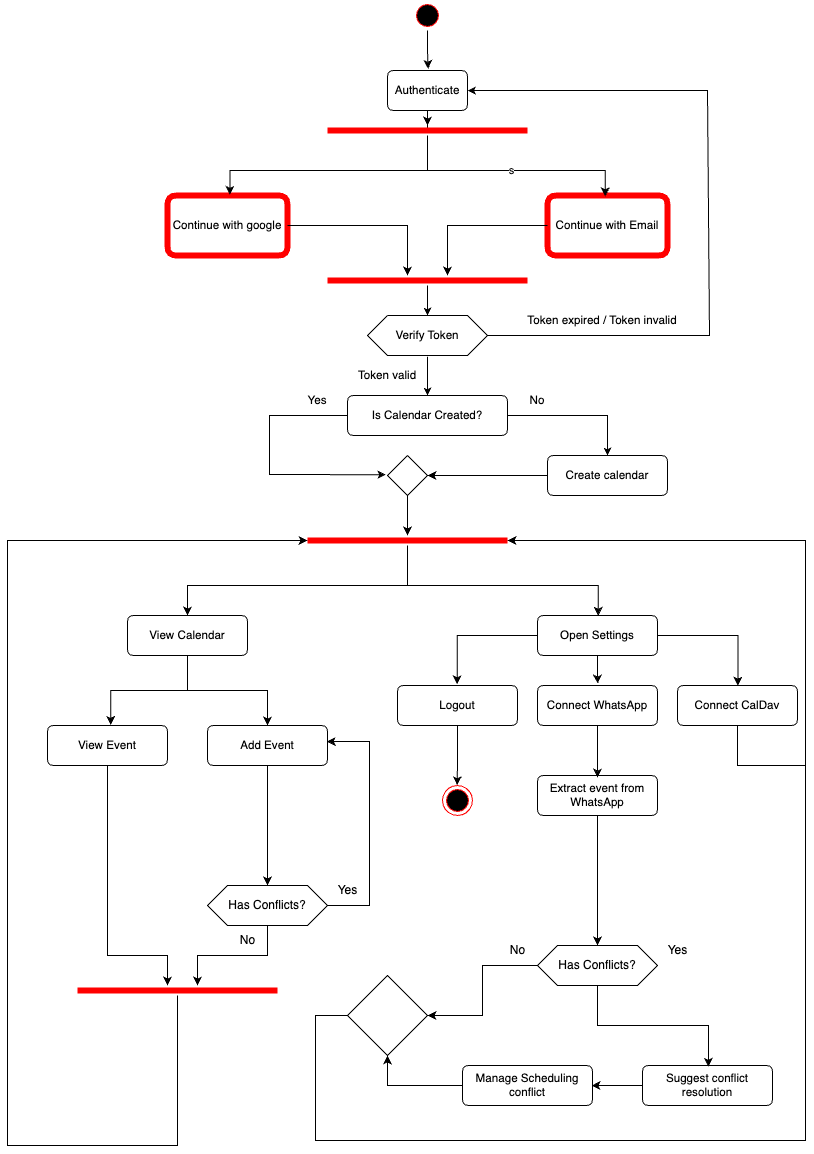
\includegraphics[width=0.9\textwidth]{images/activity-diagram.png}
    \caption{Activity Diagram of Jadwal}
    \label{fig:activity-diagram}
\end{figure}

\newpage

An activity diagram is shown in Figure~\ref{fig:activity-diagram} above, and it illustartes the flows the user of the app can take. It starts with the authentication whcih supports both Google and Email. Then afater the token is verified, a check is done to see if the user has a calendar or not. If the user has a calendar, we just move on, but if they don't have one, we create one and then move on. Here the user is inside the app and has two options, he can either view the calendar or open the settings page. When he views the calendar, he can view an event, or add one. Adding event might result in a conflict, so if one arises, they can try editing it and adding it again til no conflicts arise. After any of those two steps, the user can go back to view calendar or open settings page. If the choose to open settings page, they have three actions available. They can connect a CalDAV account, connect WhatsApp, or logout. Starting with the connecting a WhatsApp account, the system will extract events from the user's WhatsApp account automatically. If any conflicts arise, the system suggests a conflict resolution, and the user can take action by managing the scheduling conflict. But if no conflicts arise, the system just continues normally. Another option for the user is connecting a CalDAV account, and once that happens, the user can go back to having the option of going to calendar view or open settings page. Finally, the logout action and that terminates the session and the user is logged out of the app.



\section{Class Diagram}

The figures below show the main classes Jadwal's system includes. The figures give an overview of interfaces in the system to help in understanding the different parts of the system. Since Golang will be used for the backend mainly, the diagrams below are more suited for it.

Of course that doesn't mean they can't be used for implementing in other languages, but the way it was written took into consideration the language features. Golang is neither fully object oriented neither fully functional. It has \texttt{interface} and \texttt{struct}, and has implicit implementation. Implicit implementation means as long as a struct has the methods that an interface expects, that struct implemented the interface. Below is a key for the class diagrams coming below:
\begin{itemize}
    \item S - \texttt{struct} (Go struct type)
    \item T - \texttt{type} (Go type definition)
    \item C - \texttt{class} (Go interface implementations)
    \item I - \texttt{interface} (Go interface definition)
\end{itemize}

\newpage

\begin{figure}[!h]
    \centering
    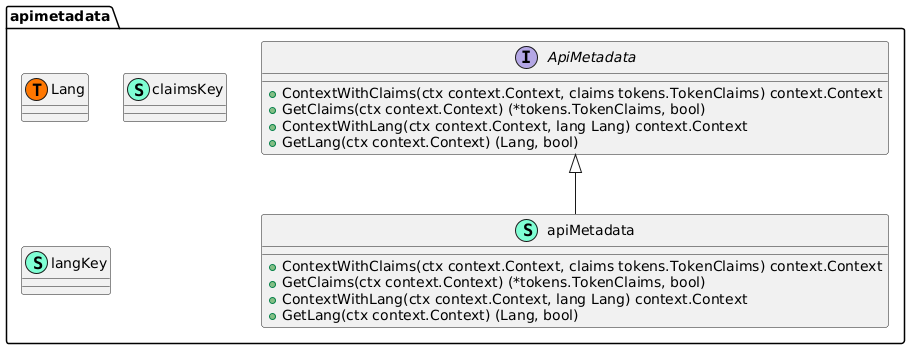
\includegraphics[width=0.9\textwidth]{images/docs/diagrams/class/class-diagram/apimetadata.png}
    \caption{Api Metadata Class Diagram}
    \label{fig:api-metadata-class-diagram}
\end{figure}

In Figure~\ref{fig:api-metadata-class-diagram}, the diagram shows the Api Metadata interface and its implementation along with important fields. It basically extracts data from the headers and includes it in the context of the requests. It helps you put stuff into the context and extract it from them. Context in Golang allows you to attach stuff to it, but it is not type safe, so we are making a wrapper to make it safe. Below we are adding wrappers for \texttt{Claims} and \texttt{Lang}. \texttt{Claims} are extracted from the JWT (JSON Web Token). \texttt{Lang} is self-explanatory.

\newpage

\begin{figure}[!h]
    \centering
    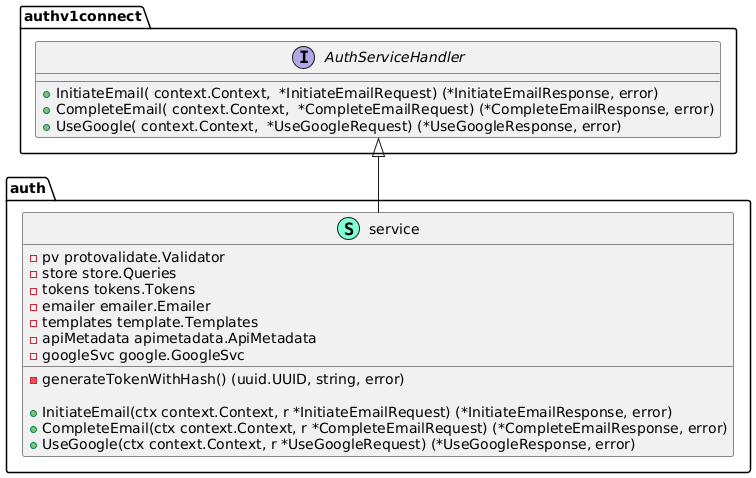
\includegraphics[width=0.9\textwidth]{images/docs/diagrams/class/class-diagram/auth.png}
    \caption{Auth Class Diagram}
    \label{fig:auth-class-diagram}
\end{figure}

In Figure~\ref{fig:auth-class-diagram}, the diagram shows the Auth API interface with its dependencies.
It also shows the \texttt{authv1connect} which is the generated code for the API\@.
This includes the flow for using email to authenticate and using Google.

\newpage

\begin{figure}[!h]
    \centering
    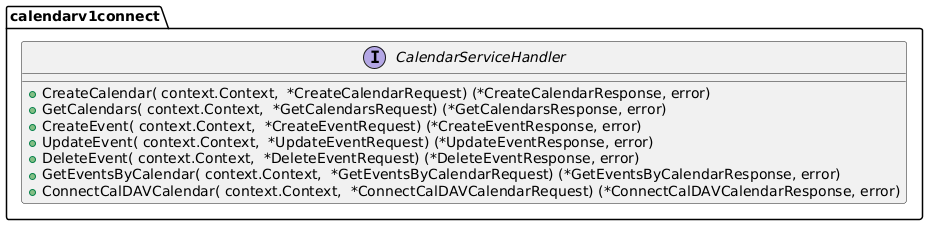
\includegraphics[width=0.9\textwidth]{images/docs/diagrams/class/class-diagram/calendarv1.png}
    \caption{Calendar V1 Class Diagram}
    \label{fig:calendar-v1-class-diagram}
\end{figure}

In Figure~\ref{fig:calendar-v1-class-diagram}, the diagram shows the api layer service calendar.
It allows Jadwal's clients to manage their calendar data easily.
It shows the interfaces and the implementation structs with their fields and methods.

\newpage

\begin{figure}[!h]
    \centering
    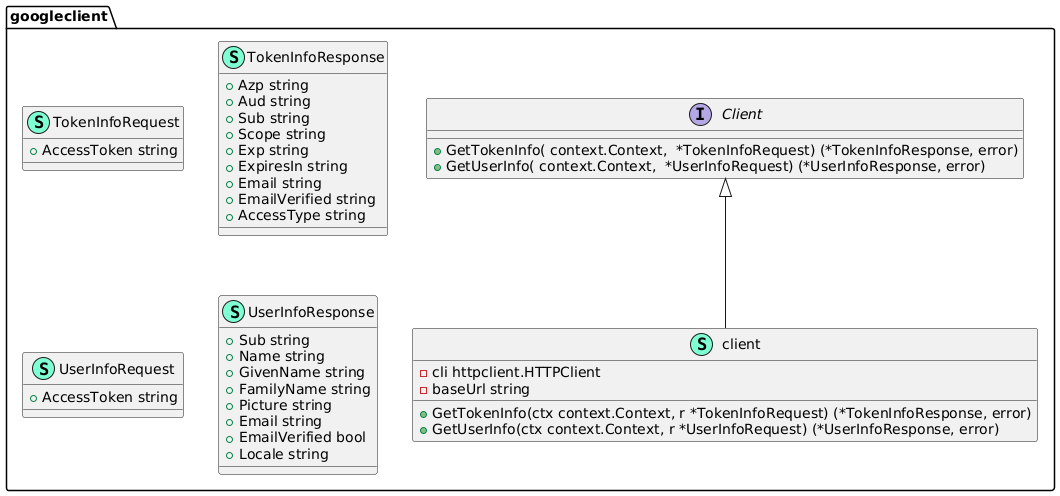
\includegraphics[width=0.9\textwidth]{images/docs/diagrams/class/class-diagram/googleclient.png}
    \caption{Google Client Class Diagram}
    \label{fig:googleclient-class-diagram}
\end{figure}

In Figure~\ref{fig:googleclient-class-diagram}, the Google client, and its methods.
It allows Jadawl to verify with Google that tokens its gets are good, and it also allows Jadwal system to get the user info the system was granted access for.

\newpage

\begin{figure}[!h]
    \centering
    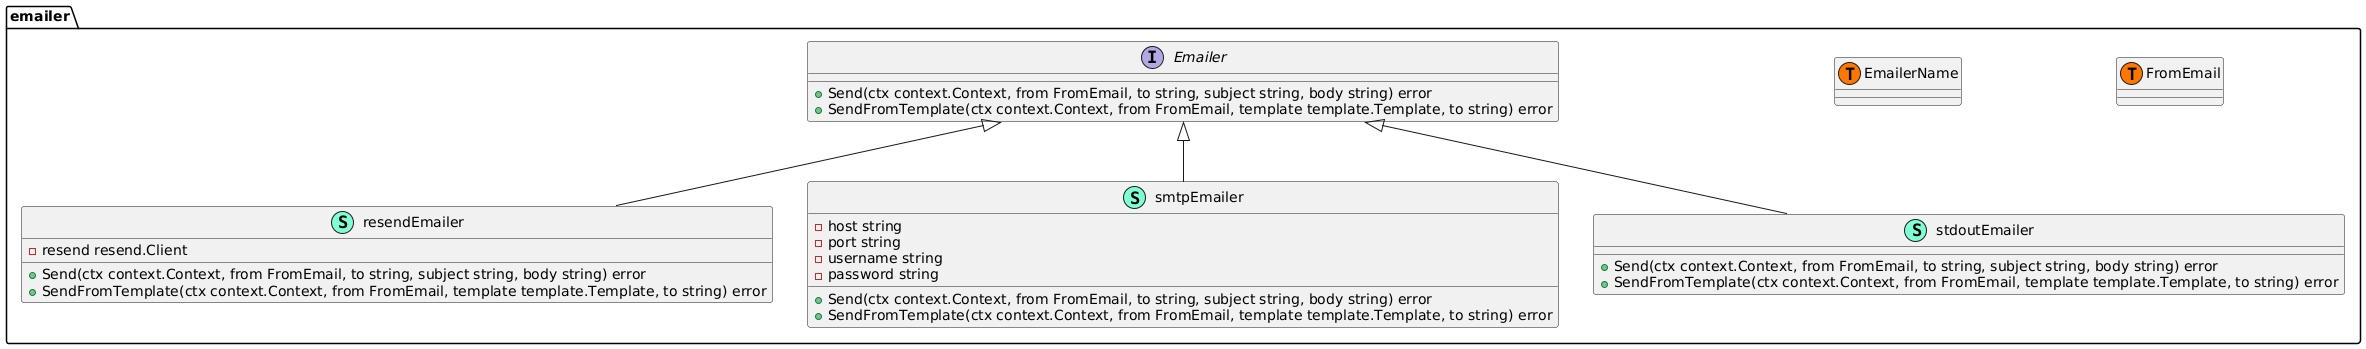
\includegraphics[width=0.9\textwidth]{images/docs/diagrams/class/class-diagram/emailer.png}
    \caption{Emailer Class Diagram}
    \label{fig:emailer-class-diagram}
\end{figure}

In Figure~\ref{fig:emailer-class-diagram}, the diagram shows the \texttt{emailer} interface with its three implementations. This allows for using the texttt{stdoutEmailer} when testing locally, and using either of the \texttt{resendEmailer} or \texttt{smtpEmailer} in production to send real emails.

\newpage

\begin{figure}[!h]
    \centering
    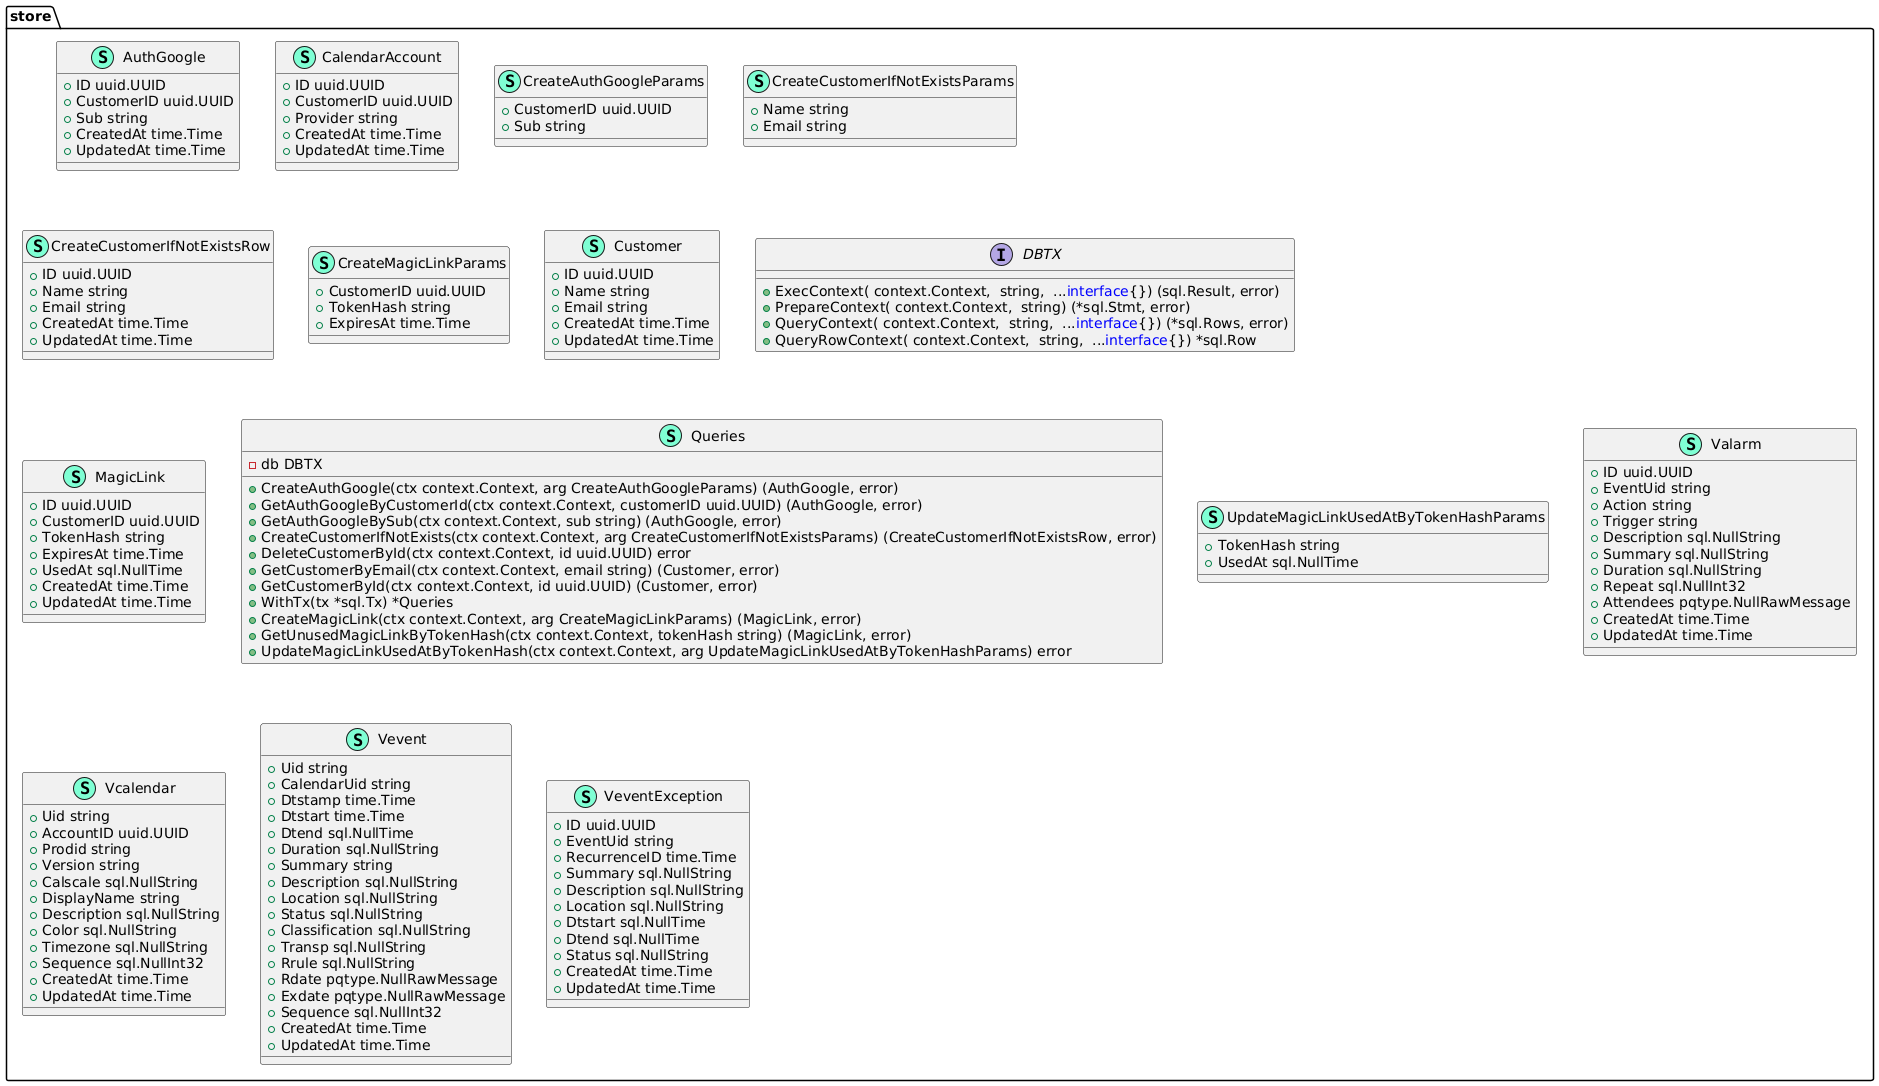
\includegraphics[width=0.9\textwidth]{images/docs/diagrams/class/class-diagram/store.png}
    \caption{Store Class Diagram}
    \label{fig:store-class-diagram}
\end{figure}

In Figure~\ref{fig:store-class-diagram}, the diagram shows the store, or in other words the database. The store holds all the methods needed to query the database for information it holds. More methods can be added as needed, but those are the core methods.

\newpage

\begin{figure}[!h]
    \centering
    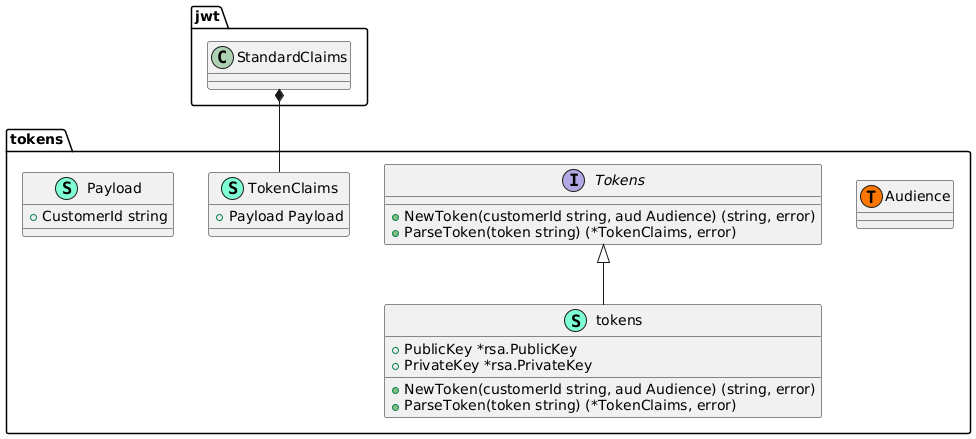
\includegraphics[width=0.9\textwidth]{images/docs/diagrams/class/class-diagram/tokens.png}
    \caption{Tokens Class Diagram}
    \label{fig:tokens-class-diagram}
\end{figure}

In Figure~\ref{fig:tokens-class-diagram}, the diagram shows the tokens service implementation along with its interface. The diagram also illustartes the needed \texttt{struct} representation for any data passed to and from the service.

\newpage

\begin{figure}[!h]
    \centering
    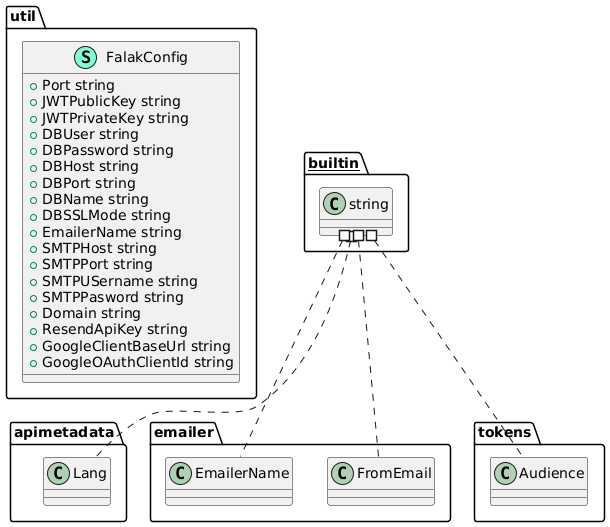
\includegraphics[width=0.5\textwidth]{images/docs/diagrams/class/class-diagram/util.png}
    \caption{Util Class Diagram}
    \label{fig:util-class-diagram}
\end{figure}

In Figure~\ref{fig:util-class-diagram}, the diagram shows config needed to support both production and development without committing secrets to the codebase. Falak in this context is the codename for the backend. The config here is represented as a \texttt{struct} since it is hold data and doesn't need implementations.

\section{Database Design}

\begin{figure}[!h]
    \centering
    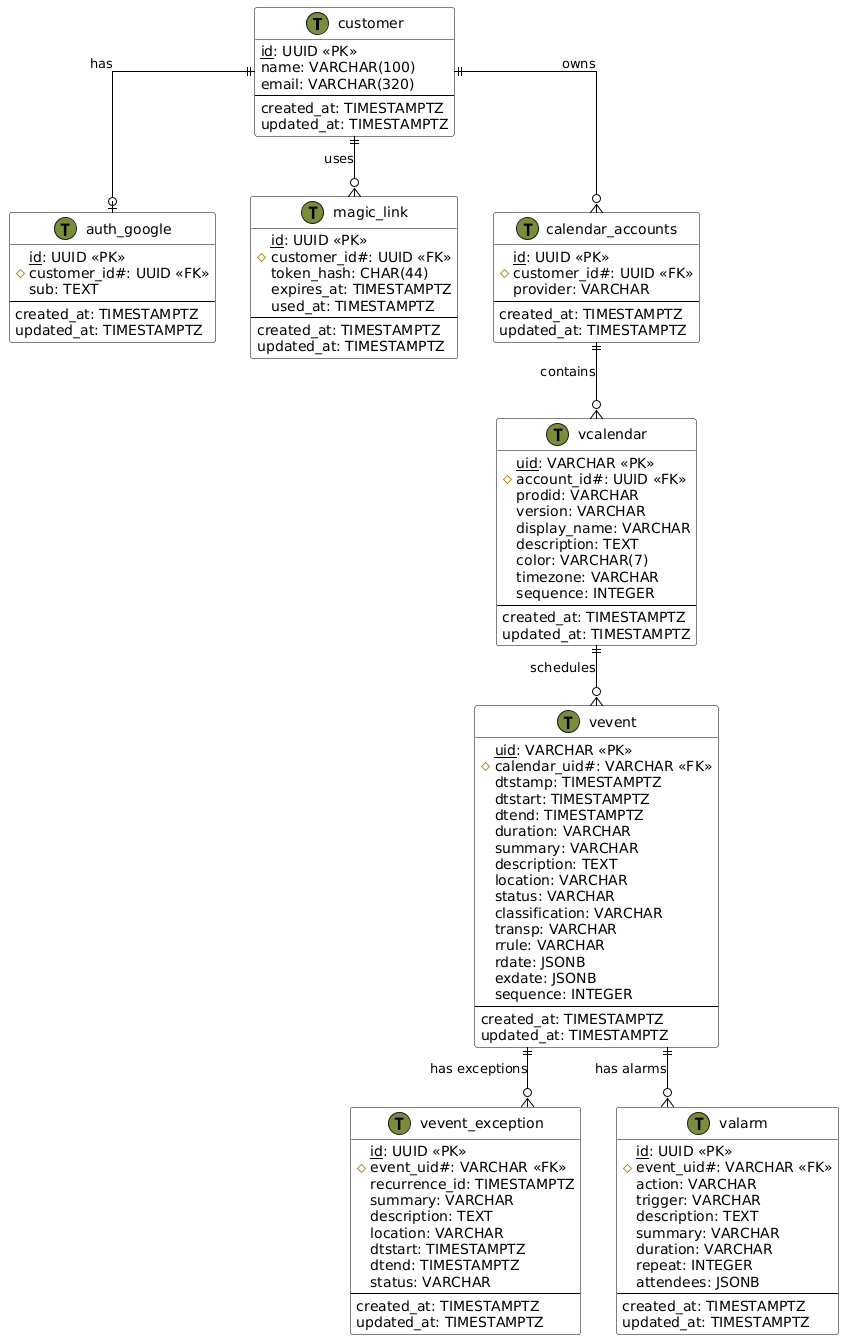
\includegraphics[width=0.9\textwidth]{images/docs/diagrams/er/database/Database Design.png}
    \caption{Database Design}
    \label{fig:database-design}
\end{figure}

\newpage

In Figure \ref{fig:database-design}, the tables and the relations between them in Jadwal's system is shown. The \texttt{customer} is the main table. Three tables have foreign keys that reference it. The \texttt{auth\_google} and \texttt{magic\_link} tables are used for auth, and they both save the info required to the authentication and hint at which authentication methods are allowed for a specific customer.

A third table related to the \texttt{customer} table is the \texttt{calendar\_accounts} table. It makes it possible to link multiple calendars to one customer under a calendar account. Then the heirarchy continues, each \texttt{calendar\_accounts} entry contains many \texttt{vcalendar} entries. And each \texttt{vcalendar} entry contains many \texttt{vevent} entries. And each \texttt{vevent} entry has exceptions and alarms related to it\\via \texttt{vevent\_exception} and \texttt{valarm} respectively.

\section{User Interface Prototype}

\begin{figure}[!h]
    \begin{minipage}{0.3\textwidth}
        \centering
        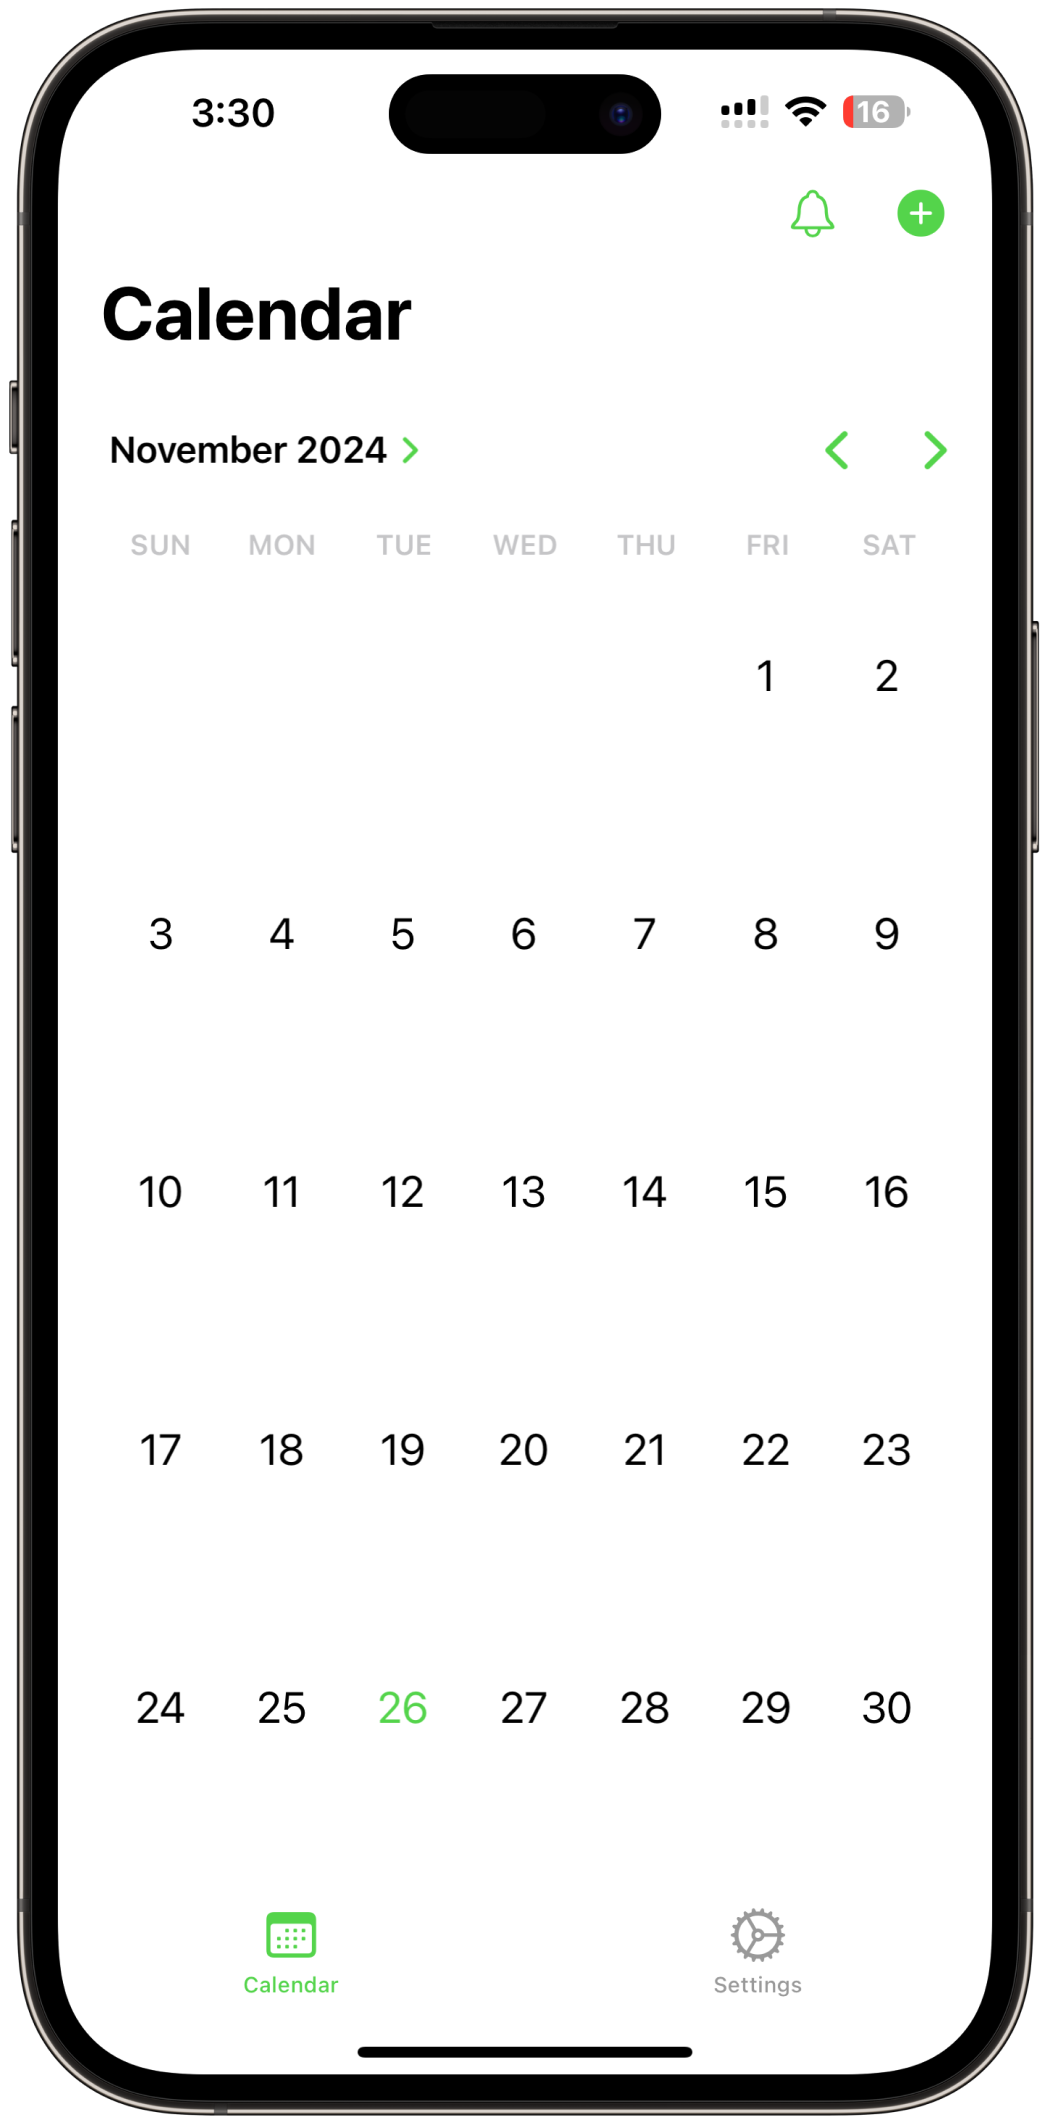
\includegraphics[width=\textwidth]{images/screen1.png}
        \caption{UI Screen 1: Onboarding View}
        \label{fig:ui-screen-1}
    \end{minipage}
    \hfill
    \begin{minipage}{0.65\textwidth}
        In Figure~\ref{fig:ui-screen-1}, the screen shows the user the steps he needs to take in the future so he knows what he is going to do. It also has two way of authenticating, Google and Email (Magic Link).
    \end{minipage}
\end{figure}

\begin{figure}[!h]
    \begin{minipage}{0.65\textwidth}
        In Figure~\ref{fig:ui-screen-2}, the screen is showing the continue with email screen which allows a user to enter their email, click "Continue", and receive an email if all is good.
    \end{minipage}
    \hfill
    \begin{minipage}{0.3\textwidth}
        \centering
        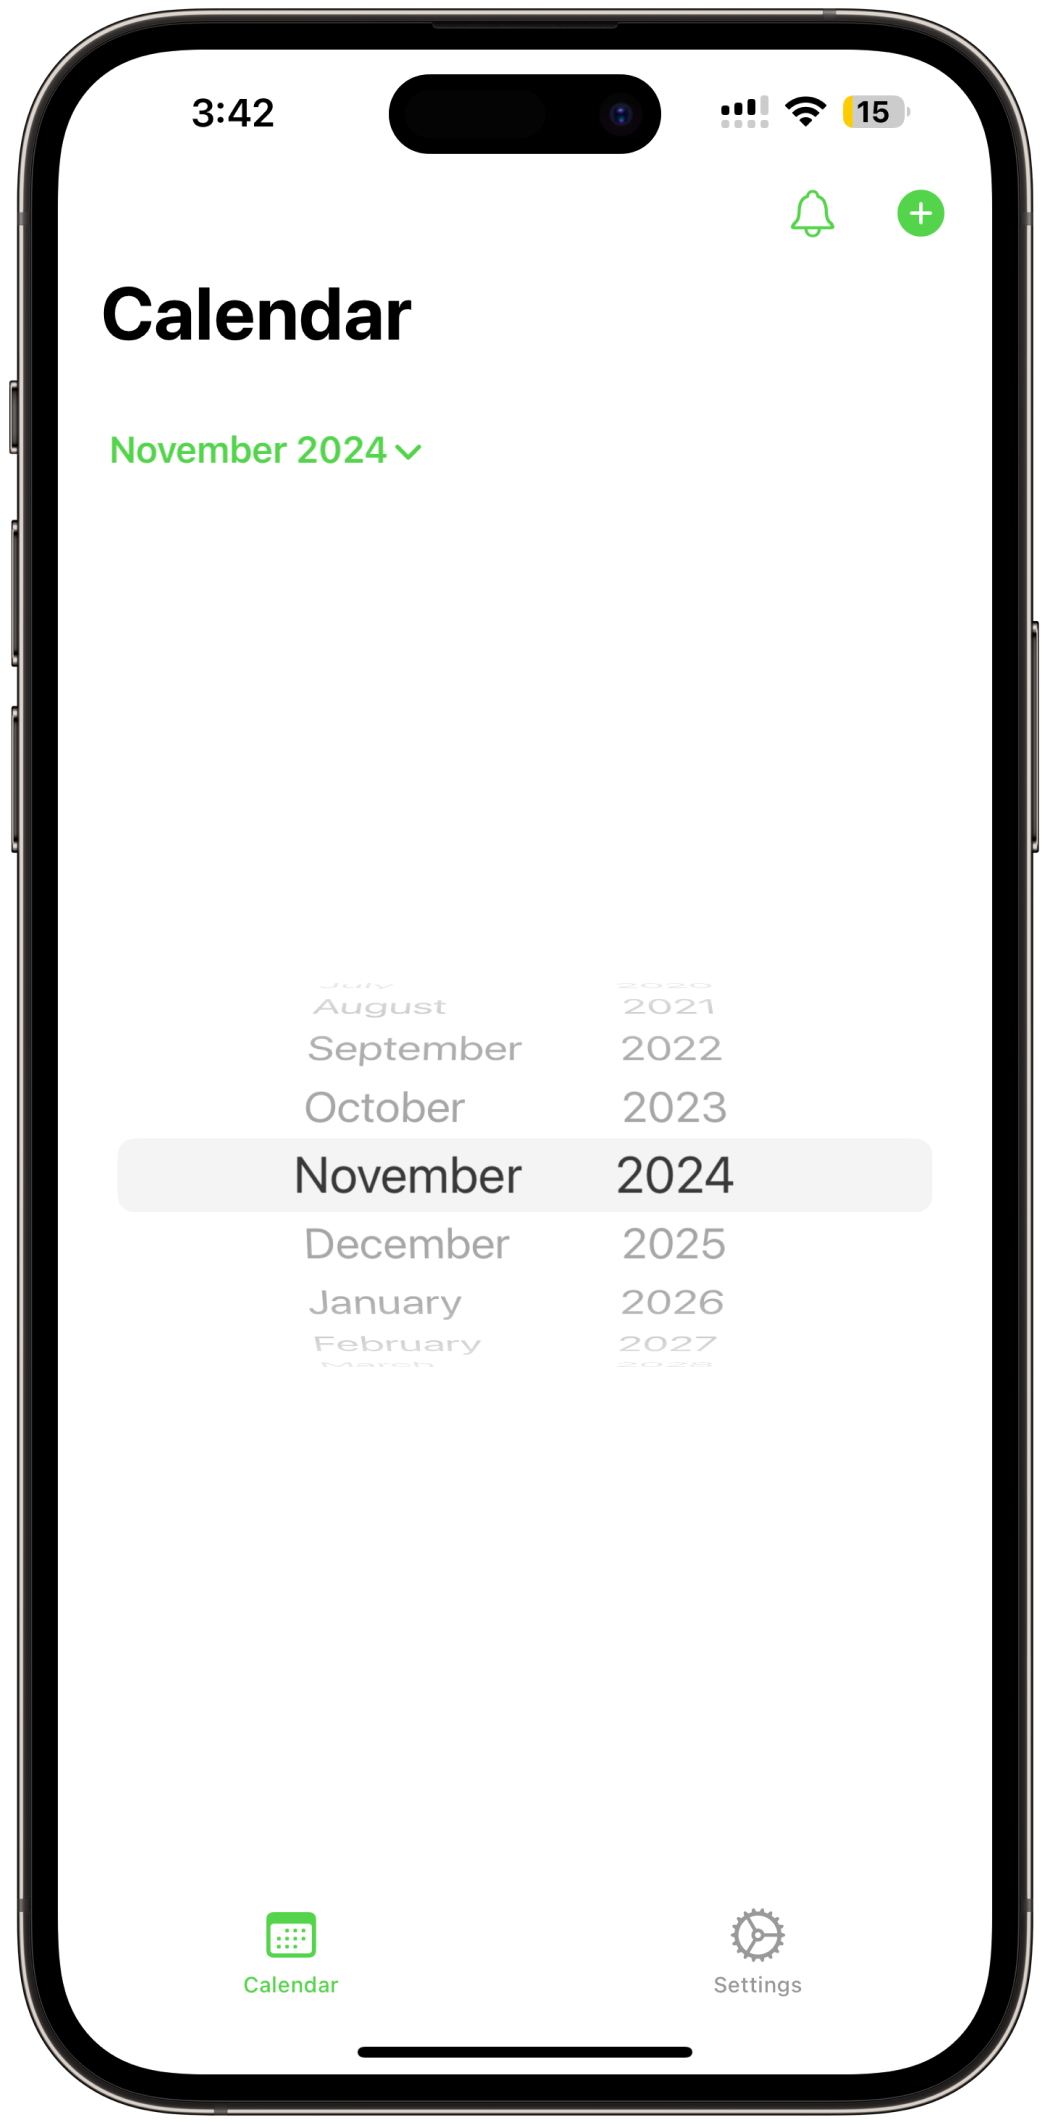
\includegraphics[width=\textwidth]{images/screen2.png}
        \caption{UI Screen 2: Continue with Email View}
        \label{fig:ui-screen-2}
    \end{minipage}
\end{figure}

\begin{figure}[!h]
    \begin{minipage}{0.3\textwidth}
        \centering
        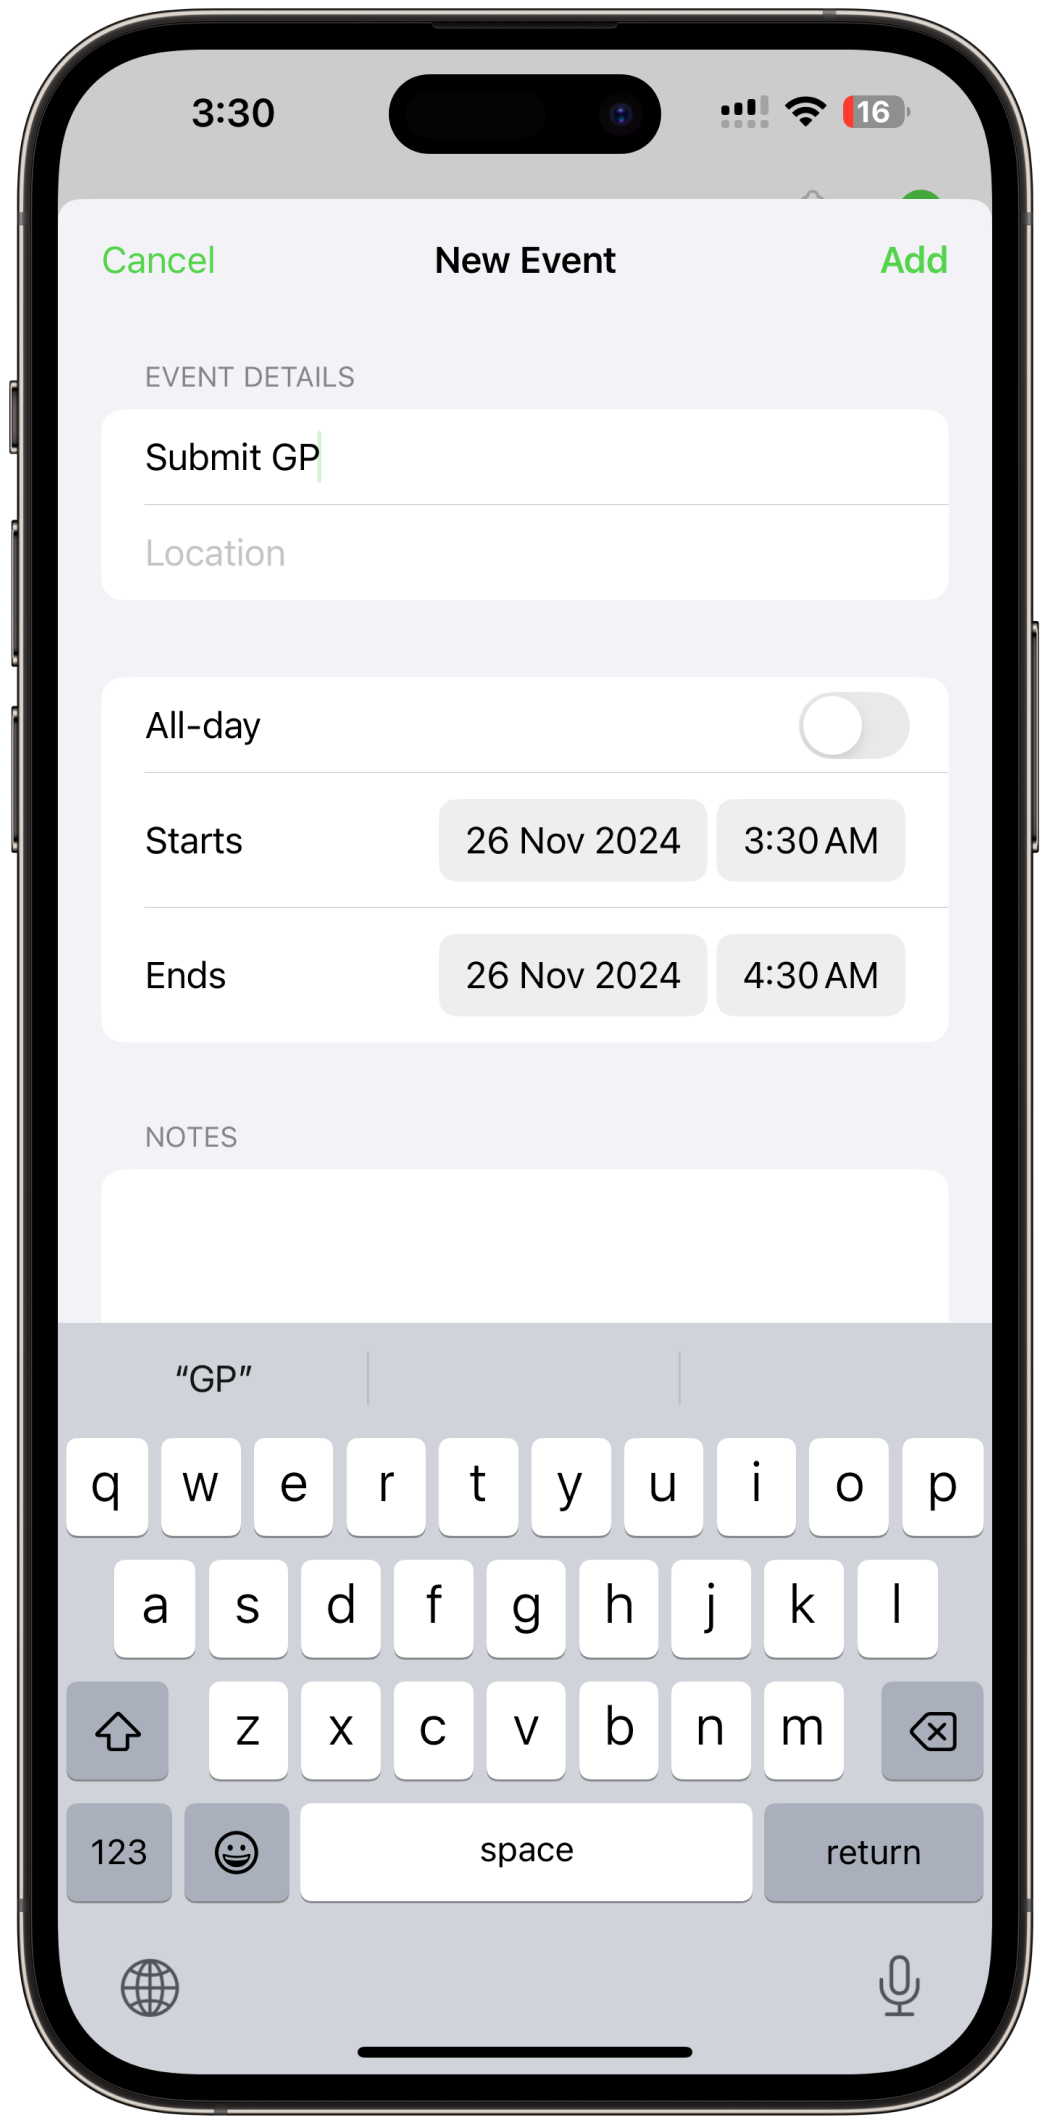
\includegraphics[width=\textwidth]{images/screen3.png}
        \caption{UI Screen 3: Check Your Email View}
        \label{fig:ui-screen-3}
    \end{minipage}
    \hfill
    \begin{minipage}{0.65\textwidth}
        In Figure~\ref{fig:ui-screen-3}, the screen that tells the user to check their email for the magic link is shown. They can also click "Resend Email" to get another copy if the first one wasn't received. If they received it, they can click the link inside it and it will redirect back to the app and the app will be able to read the url and its contents which has a token which the app uses to finish the authentication process. Once the authentication process is done, the user is moved to the screen shown in Figure~\ref{fig:ui-screen-4}
    \end{minipage}
\end{figure}

\begin{figure}[!h]
    \begin{minipage}{0.65\textwidth}
        In Figure~\ref{fig:ui-screen-4}, the calendar view represents the user's schedule. It shows upcoming events, past events, and current events. It also has two buttons at the top, notifications and add event buttons. Users can swipe left and right to navigate months. The current day is colored in green.
    \end{minipage}
    \hfill
    \begin{minipage}{0.3\textwidth}
        \centering
        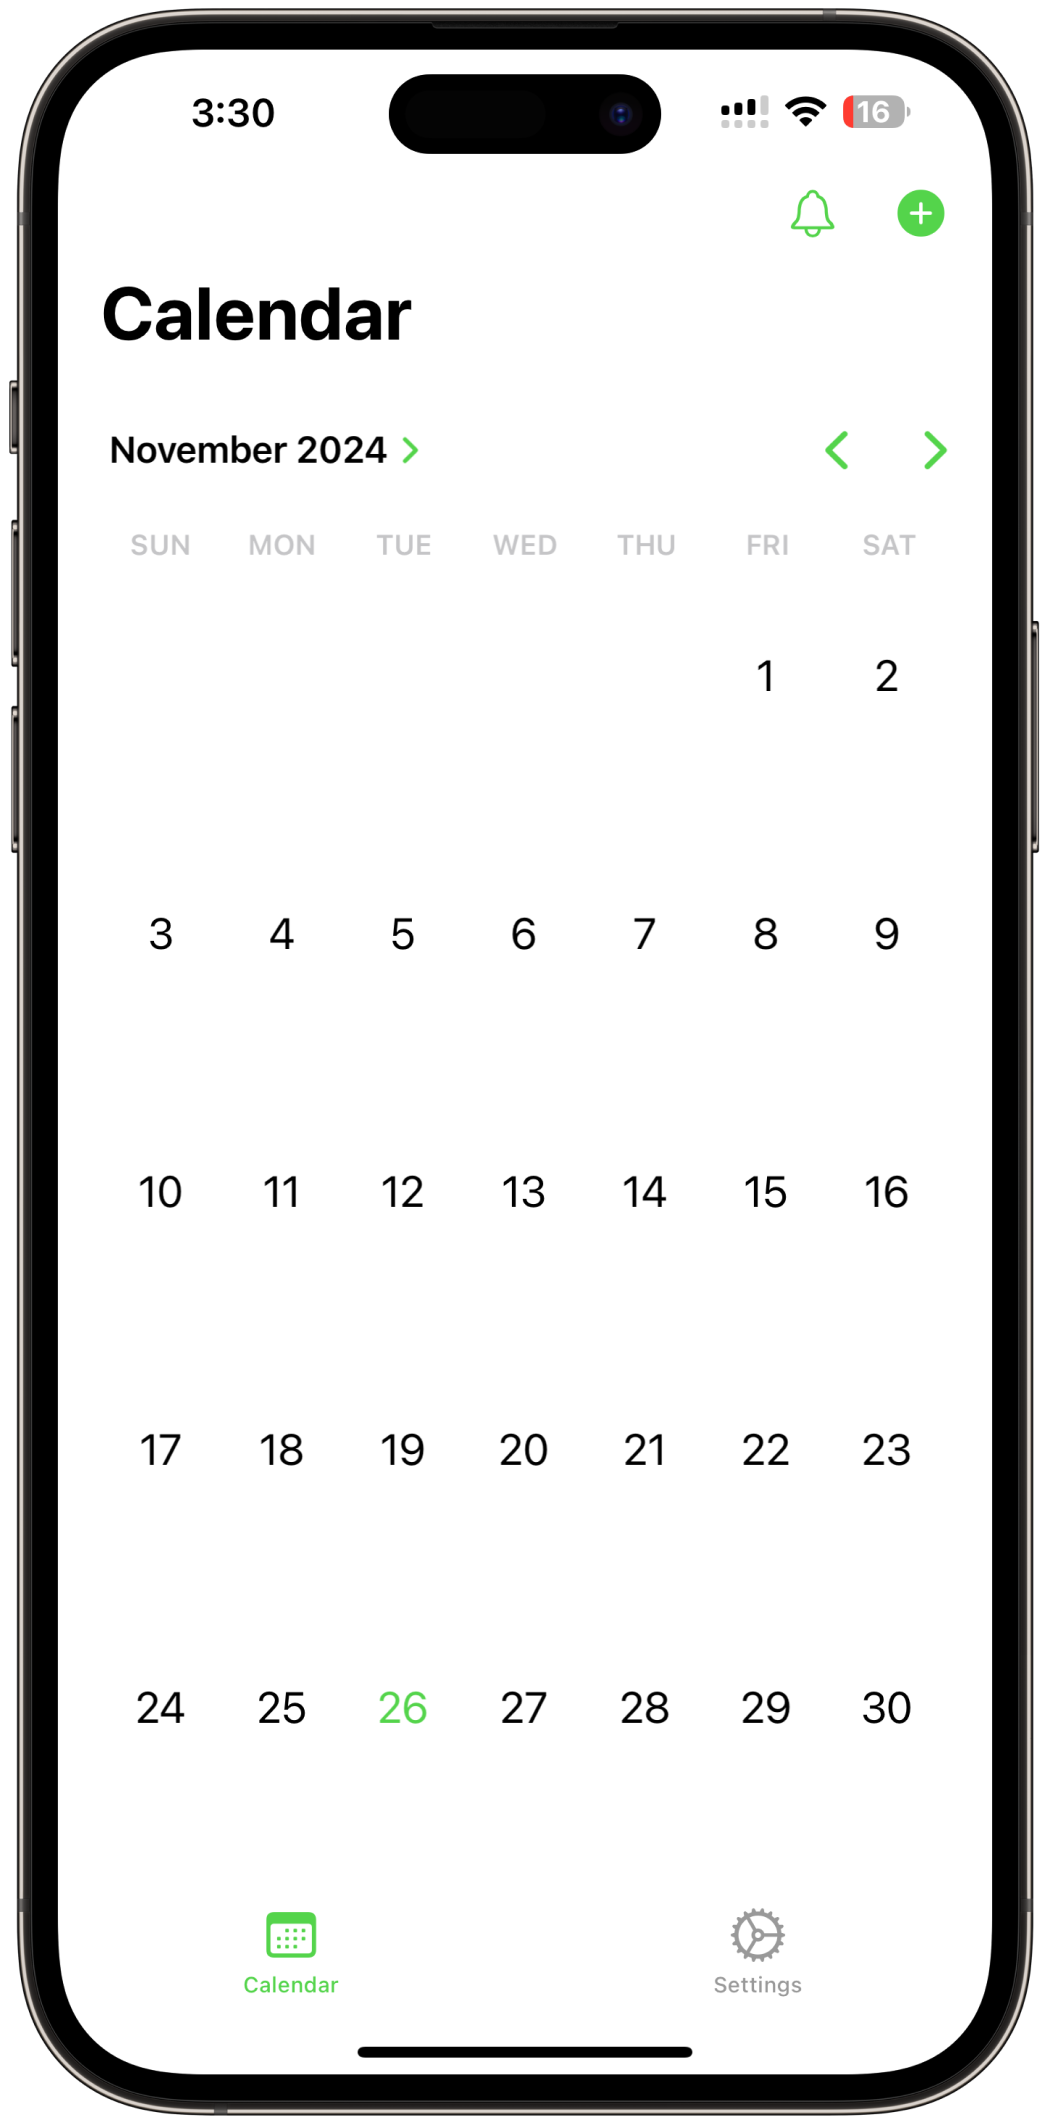
\includegraphics[width=\textwidth]{images/screen4.png}
        \caption{UI Screen 4: Calendar View}
        \label{fig:ui-screen-4}
    \end{minipage}
\end{figure}

\begin{figure}[!h]
    \begin{minipage}{0.3\textwidth}
        \centering
        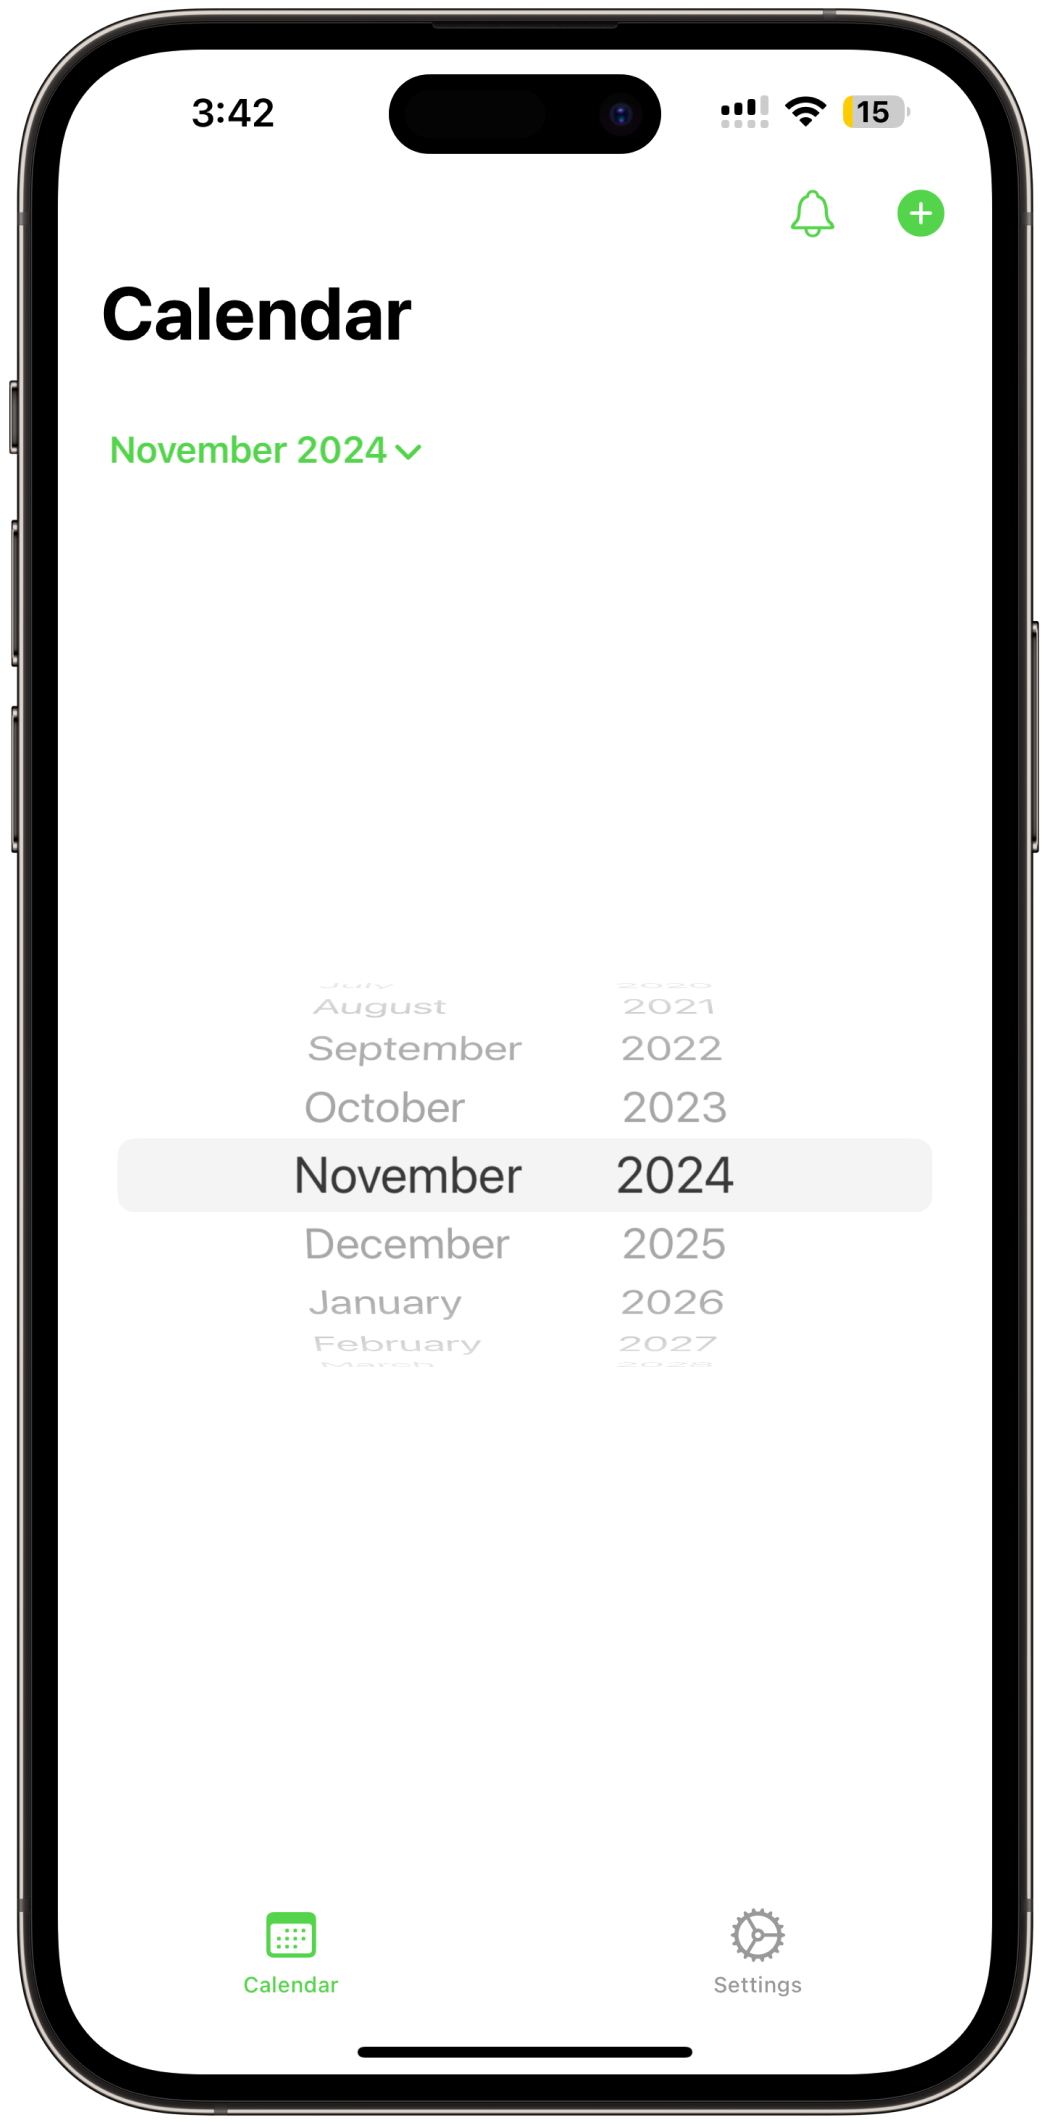
\includegraphics[width=\textwidth]{images/screen5.png}
        \caption{UI Screen 5: Month \& Year Selector}
        \label{fig:ui-screen-5}
    \end{minipage}
    \hfill
    \begin{minipage}{0.65\textwidth}
        In Figure~\ref{fig:ui-screen-5}, users can click on the text that shows the currently selected month, in this case ``November 2024'' and get a selector wheel that allows them to choose a month and a year to navigate to.
    \end{minipage}
\end{figure}

\begin{figure}[!h]
    \begin{minipage}{0.65\textwidth}
        In Figure~\ref{fig:ui-screen-6}, the screen is showing the add event sheet in its default state. It is shown when you click the "add event" button in Figure~\ref{fig:ui-screen-4}.
    \end{minipage}
    \hfill
    \begin{minipage}{0.3\textwidth}
        \centering
        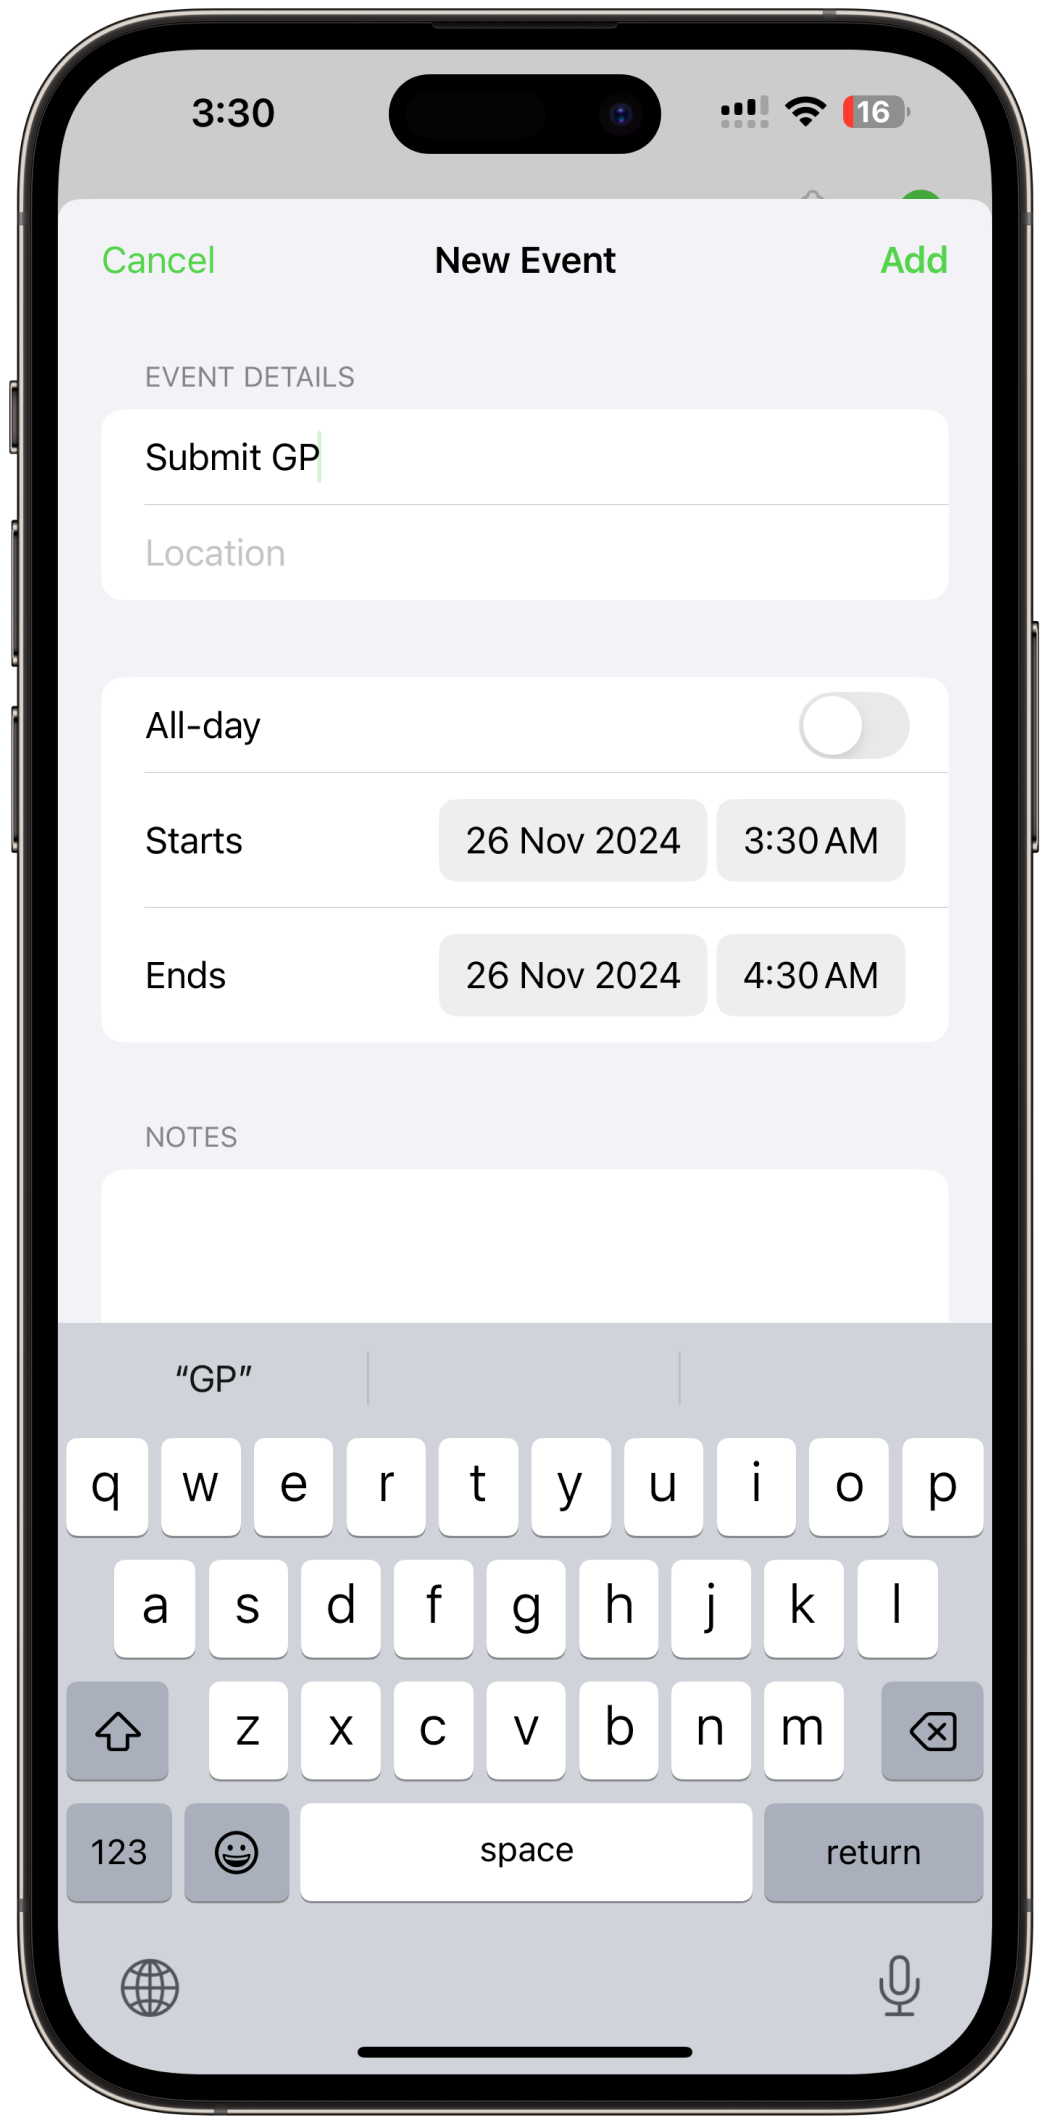
\includegraphics[width=\textwidth]{images/screen6.png}
        \caption{UI Screen 6: Add Event View - Default}
        \label{fig:ui-screen-6}
    \end{minipage}
\end{figure}

\begin{figure}[!h]
    \begin{minipage}{0.3\textwidth}
        \centering
        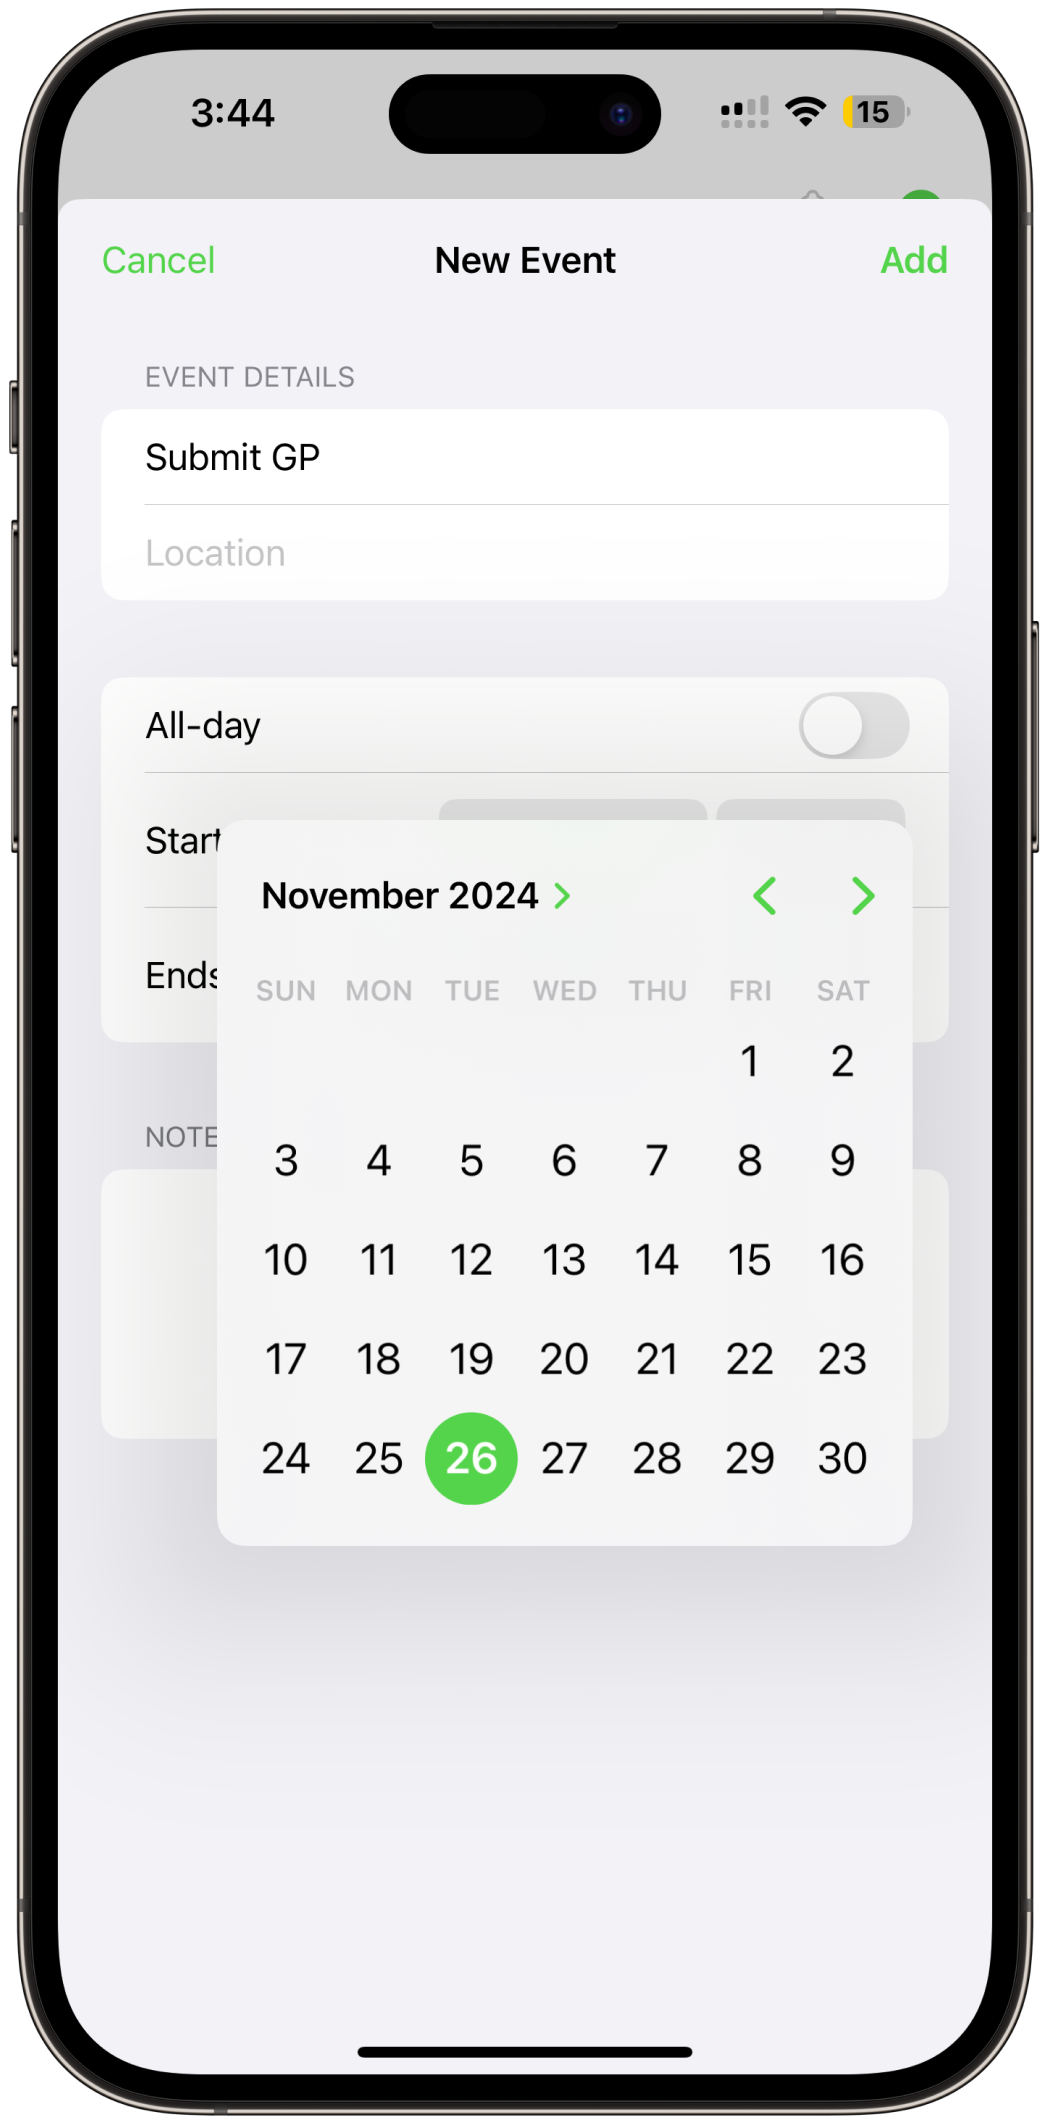
\includegraphics[width=\textwidth]{images/screen7.png}
        \caption{UI Screen 7: Add Event View - Date Picker}
        \label{fig:ui-screen-7}
    \end{minipage}
    \hfill
    \begin{minipage}{0.65\textwidth}
        In Figure~\ref{fig:ui-screen-7}, the screen is showing the add event sheet in its date picker chosen state. You can choose a date and scroll between months and years if you want.
    \end{minipage}
\end{figure}

\begin{figure}[!h]
    \begin{minipage}{0.65\textwidth}
        In Figure~\ref{fig:ui-screen-8}, the screen is showing the add event sheet in its time picker chosen state. You can choose a time and scroll between hours and minutes if you want.
    \end{minipage}
    \hfill
    \begin{minipage}{0.3\textwidth}
        \centering
        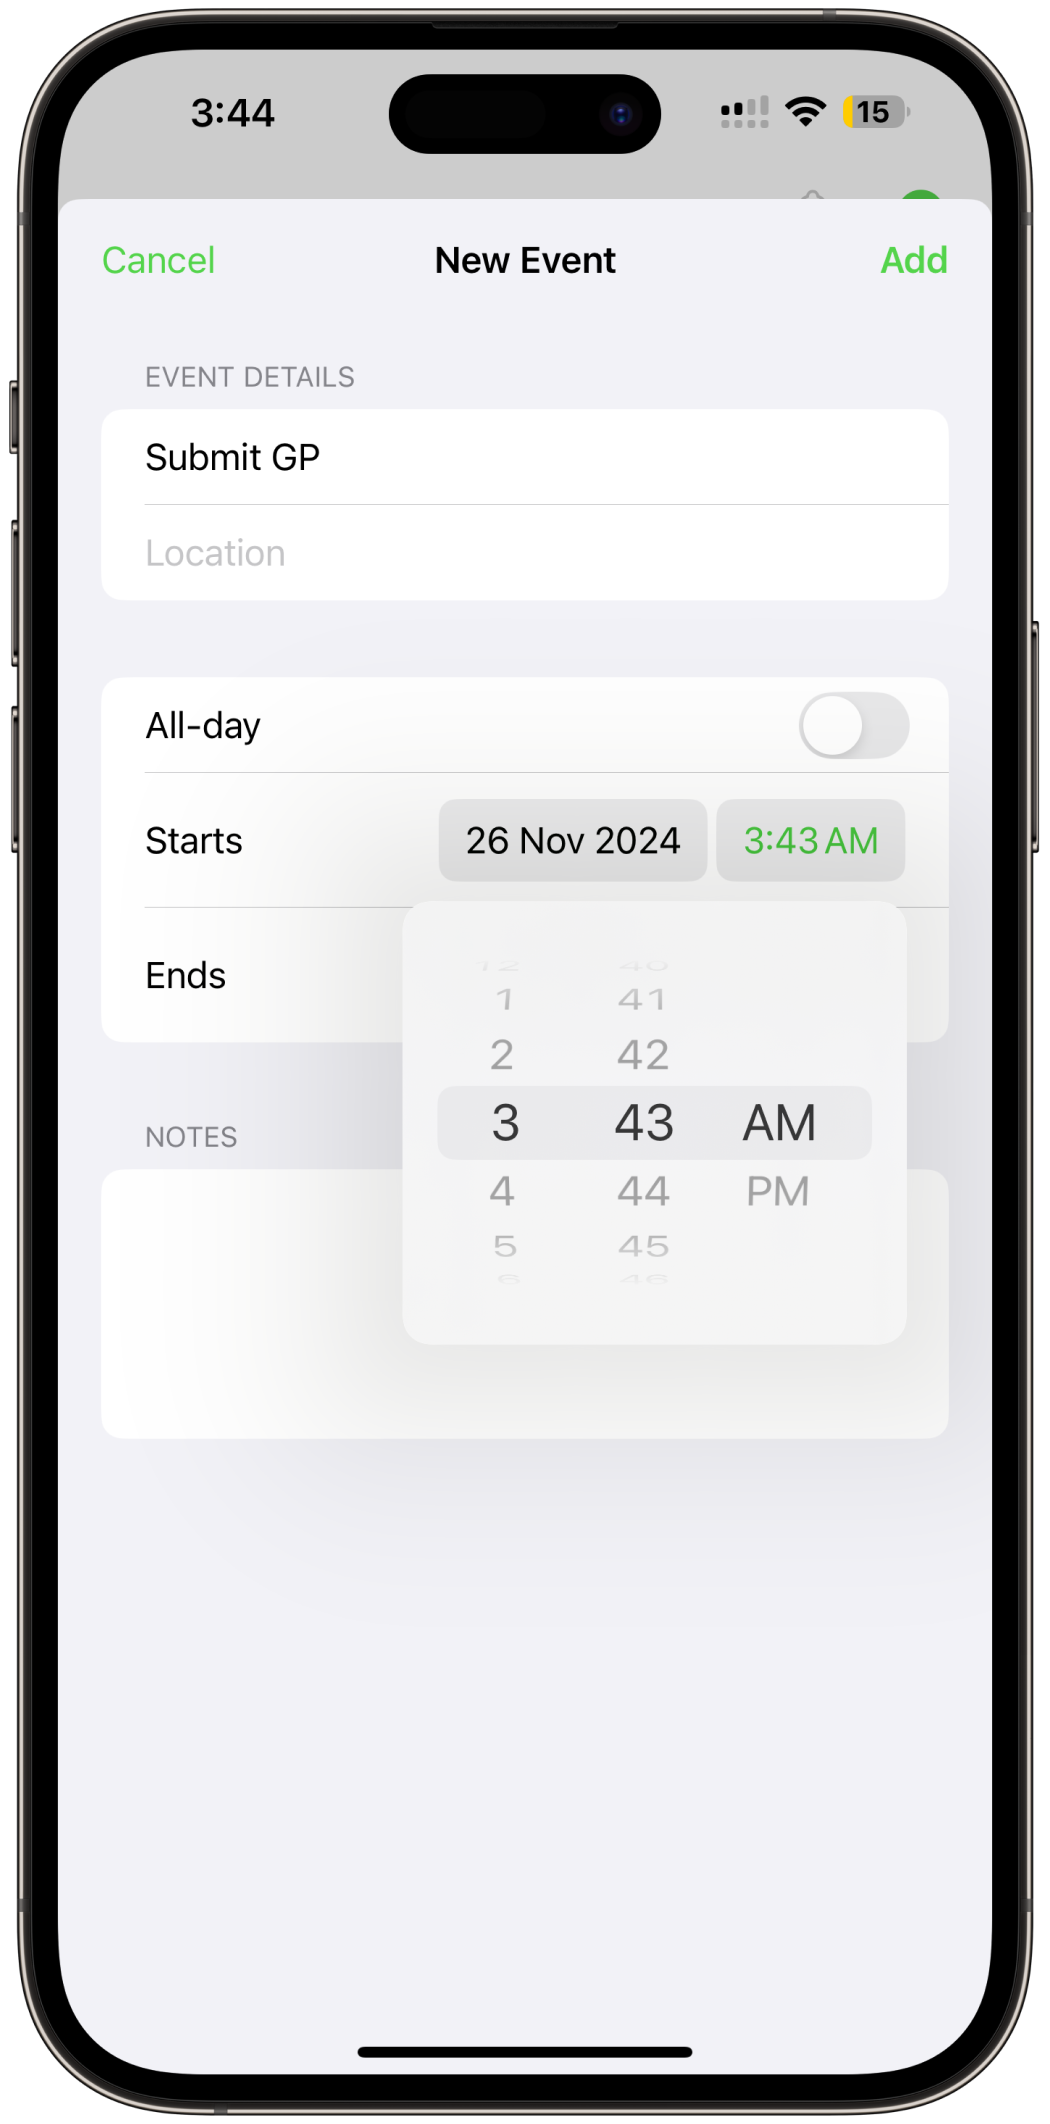
\includegraphics[width=\textwidth]{images/screen8.png}
        \caption{UI Screen 8: Add Event View - Time Picker}
        \label{fig:ui-screen-8}
    \end{minipage}
\end{figure}

\begin{figure}[!h]
    \begin{minipage}{0.3\textwidth}
        \centering
        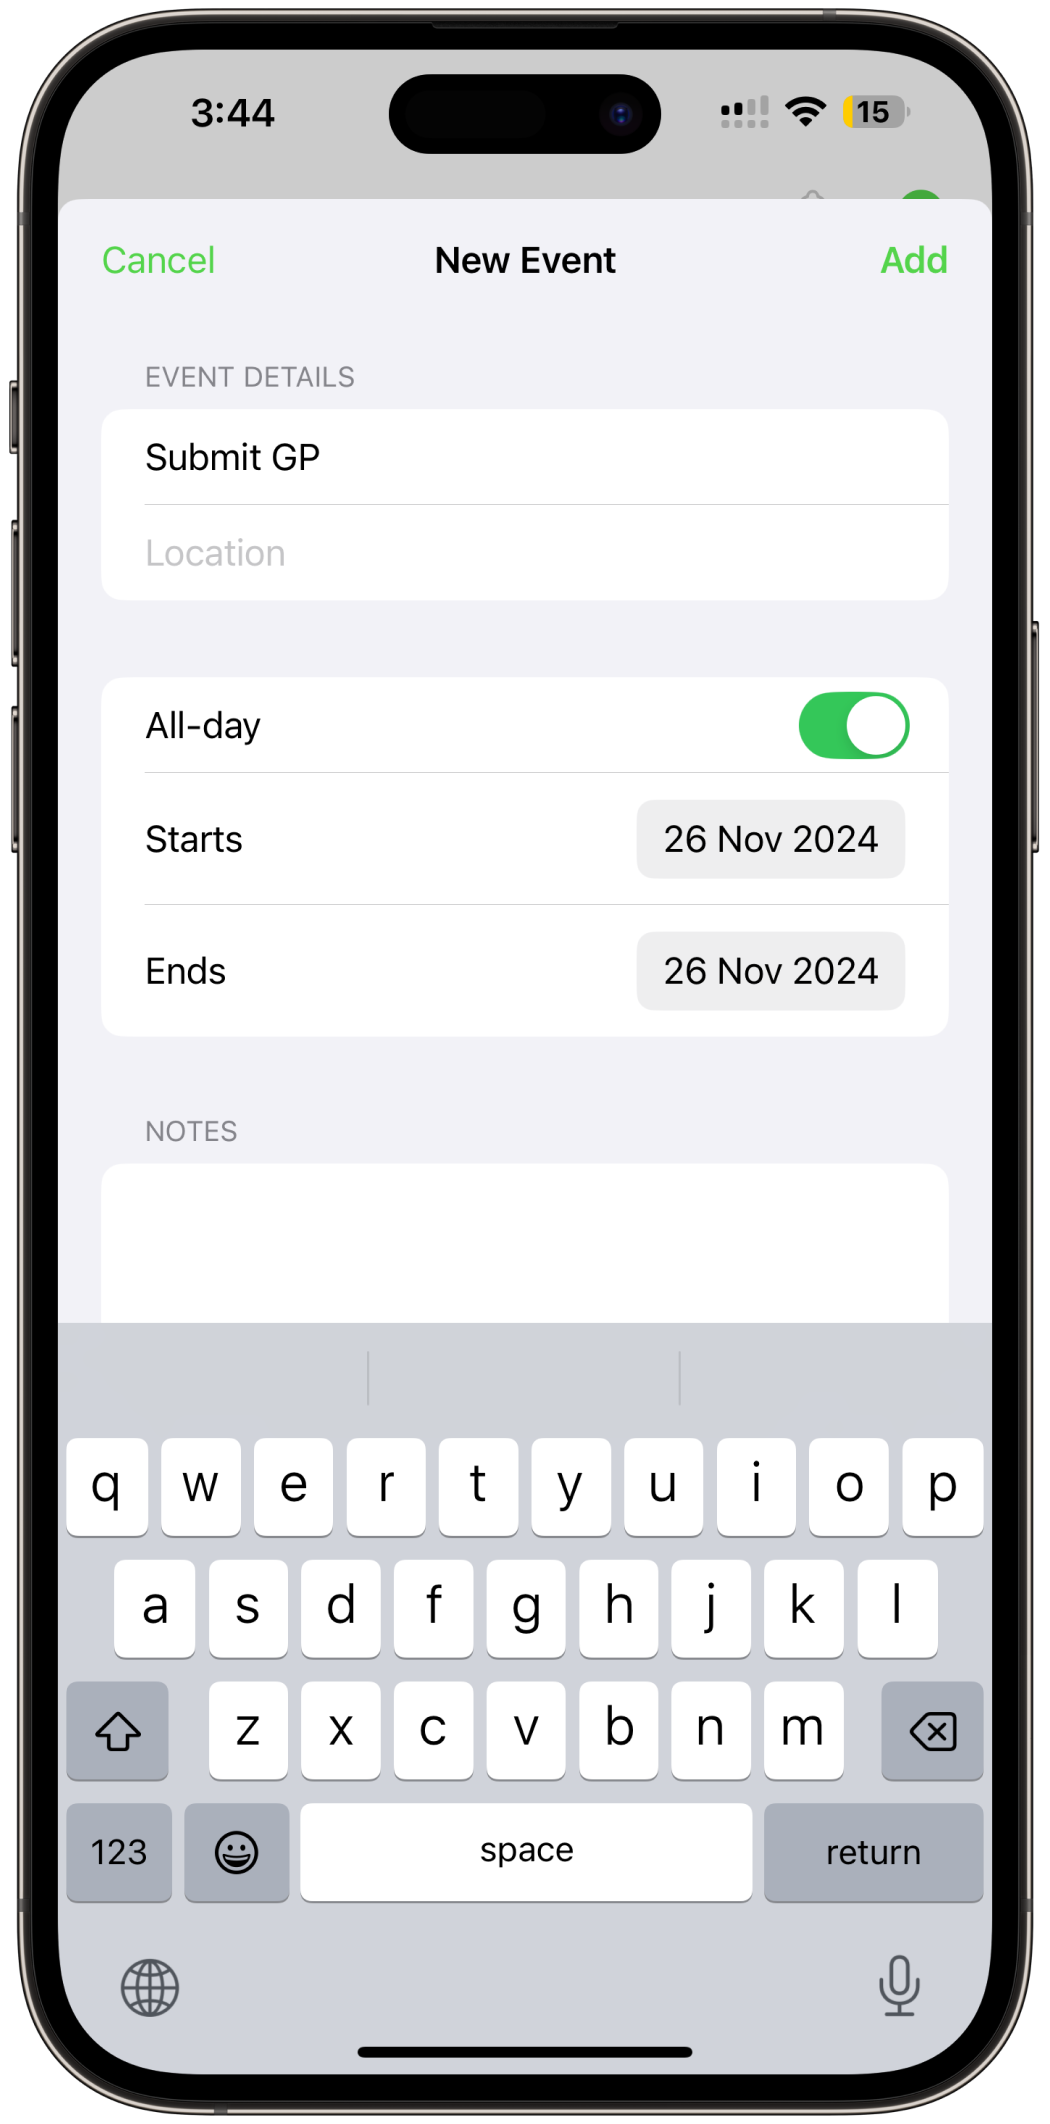
\includegraphics[width=\textwidth]{images/screen9.png}
        \caption{UI Screen 9: Add Event View - All Day}
        \label{fig:ui-screen-9}
    \end{minipage}
    \hfill
    \begin{minipage}{0.65\textwidth}
        In Figure~\ref{fig:ui-screen-9}, the screen is showing the add event sheet in its all day state. That means you only choose the dates, no need for the times.
    \end{minipage}
\end{figure}

\begin{figure}[!h]
    \begin{minipage}{0.65\textwidth}
        In Figure~\ref{fig:ui-screen-10}, the settings page is shown. This pae has the user details, specifcally email, and name. Also the "Connect WhatsApp" button is shown along with the "Connect CalDAV" button. Those two buttons do as they say and allow users to have data sources for the calendar connected. The last button shown is the logout button, and this button is in red to make the user alerted and not click it by mistake. Clicking it will log the user out and take them to the home screen.
    \end{minipage}
    \hfill
    \begin{minipage}{0.3\textwidth}
        \centering
        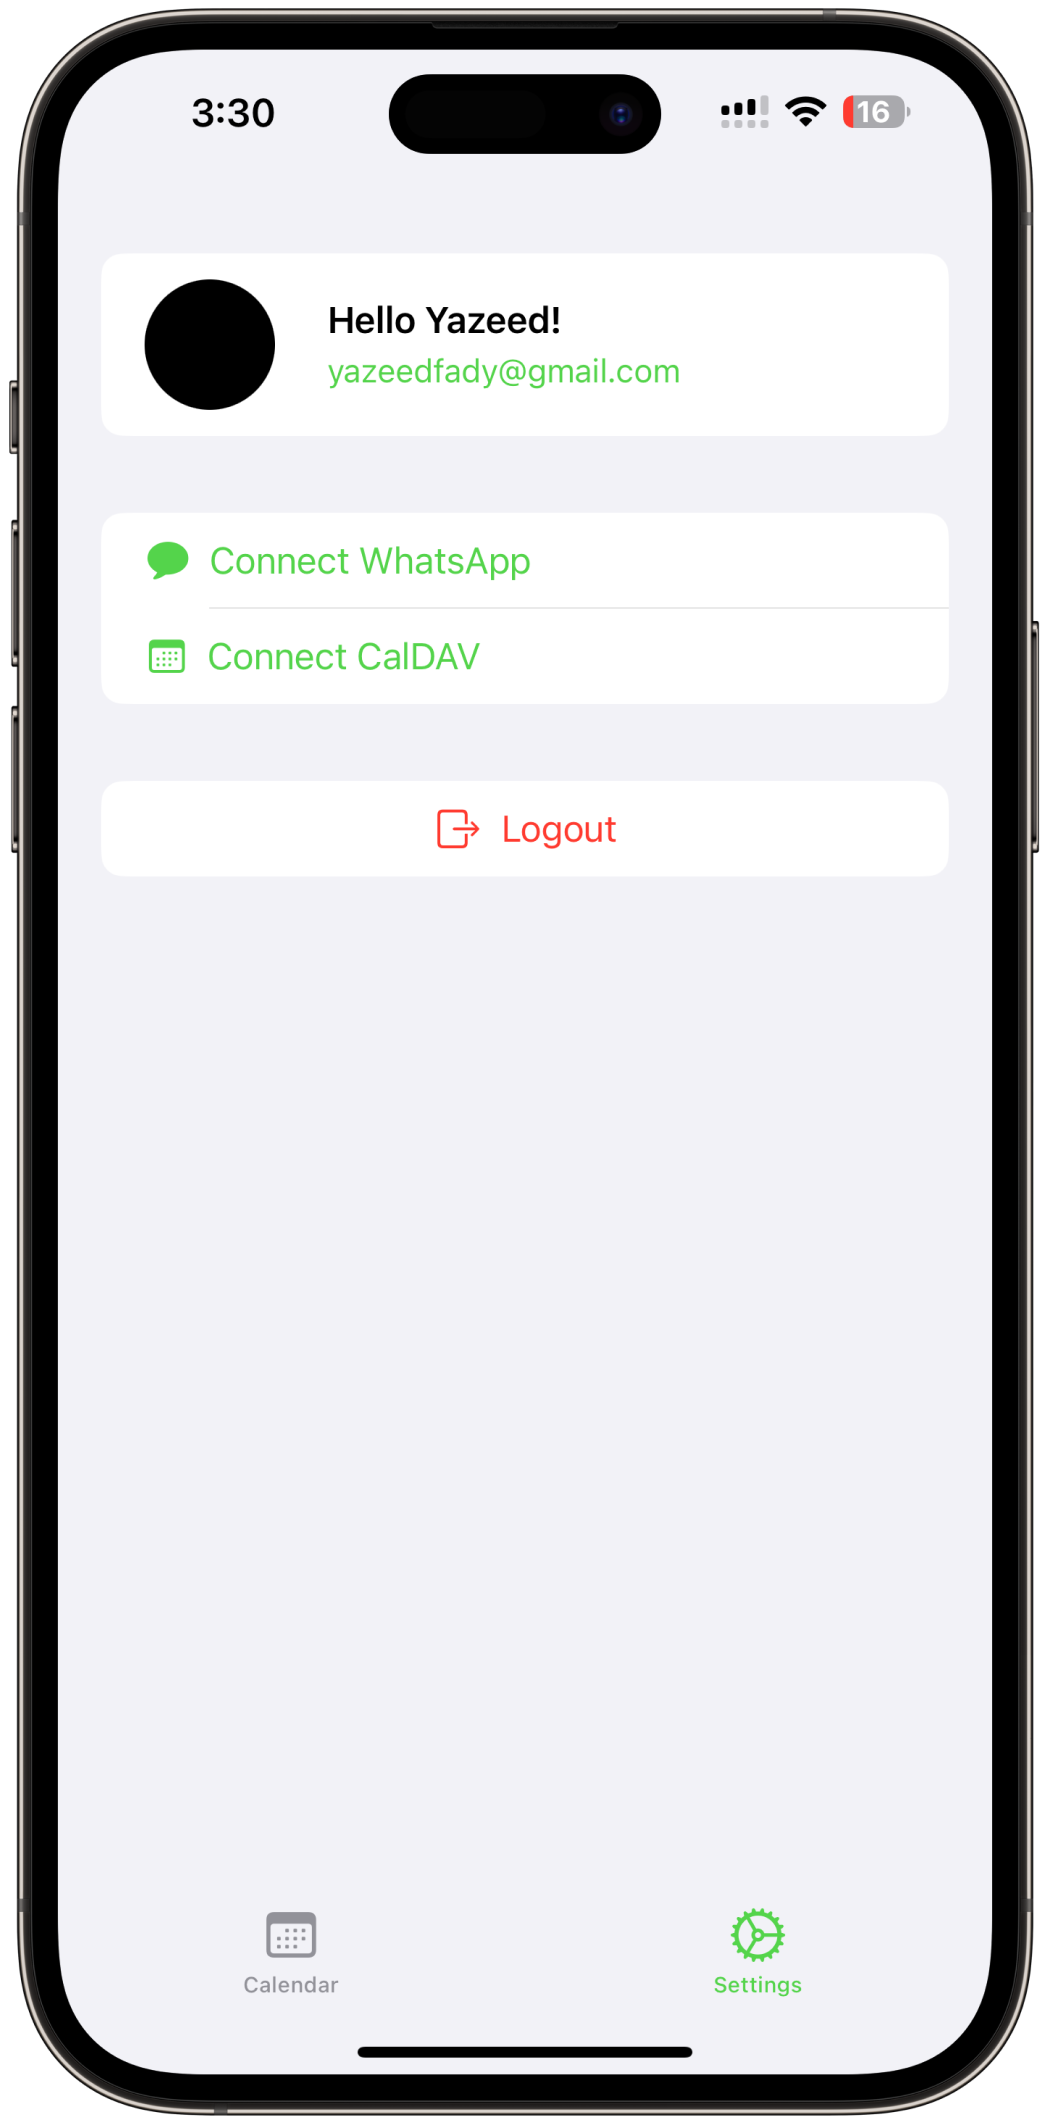
\includegraphics[width=\textwidth]{images/screen10.png}
        \caption{UI Screen 10: Settings View}
        \label{fig:ui-screen-10}
    \end{minipage}
\end{figure}

\section{Conclusion}

Jadwal stands as a comprehensive and innovative solution for scheduling with great design. The use cases and database architecture are well described that helps in creating the application systematically. The use cases clearly define how users interact with the system, covering all the features like Continue with email, Resolve conflicts, WhatsApp integration, scheduling prayer time and many more. The database design is the backbone of Jadwal, which clearly shows how the system works and how the data is managed perfectly. In conclusion, Jadwal is well described which makes it easy to understand how everything is working and would be easy to track everything that is happening in the backend. 


\chapter*{Conclusion}
\addcontentsline{toc}{chapter}{Conclusion}
\markboth{Conclusion}{}

In a fast paced and interconnected world everyone struggles to manage their time efficiently especially for someone who has multiple tasks every day. Jadwal addresses all these challenges by introducing features that helps to bridge all the gaps that other platforms are unable to offer. Jadwal ensures user friendly interface for the user to manage their schedule and avoid missing any event

Jadwal integrates with CalDAV, a standardized protocol that facilitates seamless synchronization across various calendar platforms. This allows the users to effortlessly connect and manage their calendars from different devices and applications, such as Apple Calendar and Google Calendar, making everything in one ecosystem. 

Jadwal's feature state-of-the-art LLM WhatsApp event extraction enhances the application that extract events from WhatsApp which is informal communication channel and people most likely uses it for discussing events which creates a gap that could lead to missing or conflicting an event. Jadwal aims to solve this problem.

The feature scheduling of prayer times highlights Jadwal as it is unique and Jadwal sees it important as it is a daily activity and clearing and holding place for this event would help the user to manage their day more efficiently.

The feature that makes Jadwal stand out is managing events effectively by offering features like suggesting conflict resolution and integrating other calendars. This would reduce the chances of the user missing any event.

Integration with CalDav allows Jadwal to connect all the calendars that the user has and bring it to one platform. Which helps a lot in managing the day. Why do we separate calendars to organize one day for one person. 

In conclusion, Jadwal stands out from all the existing solutions and provides an innovative calendar application that bridges the gaps and helps the user to manage their day more efficiently.


% Bibliography
\bibliography{references}
\bibliographystyle{apalike}

\end{document}